%%
%% This is file `sample-sigconf.tex',
%% generated with the docstrip utility.
%%
%% The original source files were:
%%
%% samples.dtx  (with options: `sigconf')
%% 
%% IMPORTANT NOTICE:
%% 
%% For the copyright see the source file.
%% 
%% Any modified versions of this file must be renamed
%% with new filenames distinct from sample-sigconf.tex.
%% 
%% For distribution of the original source see the terms
%% for copying and modification in the file samples.dtx.
%% 
%% This generated file may be distributed as long as the
%% original source files, as listed above, are part of the
%% same distribution. (The sources need not necessarily be
%% in the same archive or directory.)
%%
%%
%% Commands for TeXCount
%TC:macro \cite [option:text,text]
%TC:macro \citep [option:text,text]
%TC:macro \citet [option:text,text]
%TC:envir table 0 1
%TC:envir table* 0 1
%TC:envir tabular [ignore] word
%TC:envir displaymath 0 word
%TC:envir math 0 word
%TC:envir comment 0 0
%%
%%
%% The first command in your LaTeX source must be the \documentclass
%% command.
%%
%% For submission and review of your manuscript please change the
%% command to \documentclass[manuscript, screen, review]{acmart}.
%%
%% When submitting camera ready or to TAPS, please change the command
%% to \documentclass[sigconf]{acmart} or whichever template is required
%% for your publication.
%%
%%
\documentclass[acmsmall,screen]{acmart} % review option adds line numbers, screen adds colored links
\pdfoutput = 1 % [TW] Added
%%
%% [TW] toggle for switching between oopsla25 and arxiv version
%% arxiv = true means full version, arxiv = false means published conference version
\usepackage{etoolbox}
\newtoggle{arxiv}
\settoggle{arxiv}{true}

%% \BibTeX command to typeset BibTeX logo in the docs
\AtBeginDocument{%
  \providecommand\BibTeX{{%
    Bib\TeX}}}

%% Rights management information.  This information is sent to you
%% when you complete the rights form.  These commands have SAMPLE
%% values in them; it is your responsibility as an author to replace
%% the commands and values with those provided to you when you
%% complete the rights form.
% [TW] copied from publishing system
\iftoggle{arxiv}{}{
\setcopyright{acmlicensed}
\acmJournal{PACMPL}
\acmYear{2025} \acmVolume{9} \acmNumber{OOPSLA1} \acmArticle{95} \acmMonth{4}\acmDOI{10.1145/3720429}
}

\iftoggle{arxiv}{}{
%% These commands are for a PROCEEDINGS abstract or paper.
\acmConference[Conference acronym 'XX]{Make sure to enter the correct
  conference title from your rights confirmation emai}{June 03--05,
  2018}{Woodstock, NY}
%%
%%  Uncomment \acmBooktitle if the title of the proceedings is different
%%  from ``Proceedings of ...''!
%%
%%\acmBooktitle{Woodstock '18: ACM Symposium on Neural Gaze Detection,
%%  June 03--05, 2018, Woodstock, NY}
\acmISBN{978-1-4503-XXXX-X/18/06}
}


%%
%% Submission ID.
%% Use this when submitting an article to a sponsored event. You'll
%% receive a unique submission ID from the organizers
%% of the event, and this ID should be used as the parameter to this command.
%%\acmSubmissionID{123-A56-BU3}

%%
%% For managing citations, it is recommended to use bibliography
%% files in BibTeX format.
%%
%% You can then either use BibTeX with the ACM-Reference-Format style,
%% or BibLaTeX with the acmnumeric or acmauthoryear sytles, that include
%% support for advanced citation of software artefact from the
%% biblatex-software package, also separately available on CTAN.
%%
%% Look at the sample-*-biblatex.tex files for templates showcasing
%% the biblatex styles.
%%

%%
%% The majority of ACM publications use numbered citations and
%% references.  The command \citestyle{authoryear} switches to the
%% "author year" style.
%%
%% If you are preparing content for an event
%% sponsored by ACM SIGGRAPH, you must use the "author year" style of
%% citations and references.
%% Uncommenting
%% the next command will enable that style.
%\citestyle{acmauthoryear}

% from https://www.sigplan.org/Resources/Author/:
% PACMPL journal issues: \documentclass[acmsmall,screen]{acmart}. Authors can choose either author-year citations, with \citestyle{acmauthoryear}, or numeric citations, with \citestyle{acmnumeric}.
\citestyle{acmnumeric}

%% [TW] Our custom packages and macros
% basic
%\usepackage{color,xcolor}
\usepackage{color}
\usepackage{epsfig}
\usepackage{graphicx}
\usepackage{algorithm,algorithmic}
% \usepackage{algpseudocode}
%\usepackage{ulem}

% figure and table
\usepackage{adjustbox}
\usepackage{array}
\usepackage{booktabs}
\usepackage{colortbl}
\usepackage{float,wrapfig}
\usepackage{framed}
\usepackage{hhline}
\usepackage{multirow}
% \usepackage{subcaption} % issues a warning with CVPR/ICCV format
% \usepackage[font=small]{caption}
\usepackage[percent]{overpic}
%\usepackage{tikz} % conflict with ECCV format

% font and character
\usepackage{amsmath,amsfonts,amssymb}
% \let\proof\relax      % for ECCV llncs class
% \let\endproof\relax   % for ECCV llncs class
\usepackage{amsthm} 
\usepackage{bm}
\usepackage{nicefrac}
\usepackage{microtype}
\usepackage{contour}
\usepackage{courier}
%\usepackage{palatino}
%\usepackage{times}

% layout
\usepackage{changepage}
\usepackage{extramarks}
\usepackage{fancyhdr}
\usepackage{lastpage}
\usepackage{setspace}
\usepackage{soul}
\usepackage{xspace}
\usepackage{cuted}
\usepackage{fancybox}
\usepackage{afterpage}
%\usepackage{enumitem} % conflict with IEEE format
%\usepackage{titlesec} % conflict with ECCV format

% ref
% commenting these two out for this submission so it looks the same as RSS example
% \usepackage[breaklinks=true,colorlinks,backref=True]{hyperref}
% \hypersetup{colorlinks,linkcolor={black},citecolor={MSBlue},urlcolor={magenta}}
\usepackage{url}
\usepackage{quoting}
\usepackage{epigraph}

% misc
\usepackage{enumerate}
\usepackage{paralist,tabularx}
\usepackage{comment}
\usepackage{pdfpages}
% \usepackage[draft]{todonotes} % conflict with CVPR/ICCV/ECCV format



% \usepackage{todonotes}
% \usepackage{caption}
% \usepackage{subcaption}

\usepackage{pifont}% http://ctan.org/pkg/pifont

% extra symbols
\usepackage{MnSymbol}



%
\setlength\unitlength{1mm}
\newcommand{\twodots}{\mathinner {\ldotp \ldotp}}
% bb font symbols
\newcommand{\Rho}{\mathrm{P}}
\newcommand{\Tau}{\mathrm{T}}

\newfont{\bbb}{msbm10 scaled 700}
\newcommand{\CCC}{\mbox{\bbb C}}

\newfont{\bb}{msbm10 scaled 1100}
\newcommand{\CC}{\mbox{\bb C}}
\newcommand{\PP}{\mbox{\bb P}}
\newcommand{\RR}{\mbox{\bb R}}
\newcommand{\QQ}{\mbox{\bb Q}}
\newcommand{\ZZ}{\mbox{\bb Z}}
\newcommand{\FF}{\mbox{\bb F}}
\newcommand{\GG}{\mbox{\bb G}}
\newcommand{\EE}{\mbox{\bb E}}
\newcommand{\NN}{\mbox{\bb N}}
\newcommand{\KK}{\mbox{\bb K}}
\newcommand{\HH}{\mbox{\bb H}}
\newcommand{\SSS}{\mbox{\bb S}}
\newcommand{\UU}{\mbox{\bb U}}
\newcommand{\VV}{\mbox{\bb V}}


\newcommand{\yy}{\mathbbm{y}}
\newcommand{\xx}{\mathbbm{x}}
\newcommand{\zz}{\mathbbm{z}}
\newcommand{\sss}{\mathbbm{s}}
\newcommand{\rr}{\mathbbm{r}}
\newcommand{\pp}{\mathbbm{p}}
\newcommand{\qq}{\mathbbm{q}}
\newcommand{\ww}{\mathbbm{w}}
\newcommand{\hh}{\mathbbm{h}}
\newcommand{\vvv}{\mathbbm{v}}

% Vectors

\newcommand{\av}{{\bf a}}
\newcommand{\bv}{{\bf b}}
\newcommand{\cv}{{\bf c}}
\newcommand{\dv}{{\bf d}}
\newcommand{\ev}{{\bf e}}
\newcommand{\fv}{{\bf f}}
\newcommand{\gv}{{\bf g}}
\newcommand{\hv}{{\bf h}}
\newcommand{\iv}{{\bf i}}
\newcommand{\jv}{{\bf j}}
\newcommand{\kv}{{\bf k}}
\newcommand{\lv}{{\bf l}}
\newcommand{\mv}{{\bf m}}
\newcommand{\nv}{{\bf n}}
\newcommand{\ov}{{\bf o}}
\newcommand{\pv}{{\bf p}}
\newcommand{\qv}{{\bf q}}
\newcommand{\rv}{{\bf r}}
\newcommand{\sv}{{\bf s}}
\newcommand{\tv}{{\bf t}}
\newcommand{\uv}{{\bf u}}
\newcommand{\wv}{{\bf w}}
\newcommand{\vv}{{\bf v}}
\newcommand{\xv}{{\bf x}}
\newcommand{\yv}{{\bf y}}
\newcommand{\zv}{{\bf z}}
\newcommand{\zerov}{{\bf 0}}
\newcommand{\onev}{{\bf 1}}

% Matrices

\newcommand{\Am}{{\bf A}}
\newcommand{\Bm}{{\bf B}}
\newcommand{\Cm}{{\bf C}}
\newcommand{\Dm}{{\bf D}}
\newcommand{\Em}{{\bf E}}
\newcommand{\Fm}{{\bf F}}
\newcommand{\Gm}{{\bf G}}
\newcommand{\Hm}{{\bf H}}
\newcommand{\Id}{{\bf I}}
\newcommand{\Jm}{{\bf J}}
\newcommand{\Km}{{\bf K}}
\newcommand{\Lm}{{\bf L}}
\newcommand{\Mm}{{\bf M}}
\newcommand{\Nm}{{\bf N}}
\newcommand{\Om}{{\bf O}}
\newcommand{\Pm}{{\bf P}}
\newcommand{\Qm}{{\bf Q}}
\newcommand{\Rm}{{\bf R}}
\newcommand{\Sm}{{\bf S}}
\newcommand{\Tm}{{\bf T}}
\newcommand{\Um}{{\bf U}}
\newcommand{\Wm}{{\bf W}}
\newcommand{\Vm}{{\bf V}}
\newcommand{\Xm}{{\bf X}}
\newcommand{\Ym}{{\bf Y}}
\newcommand{\Zm}{{\bf Z}}

% Calligraphic

\newcommand{\Ac}{{\cal A}}
\newcommand{\Bc}{{\cal B}}
\newcommand{\Cc}{{\cal C}}
\newcommand{\Dc}{{\cal D}}
\newcommand{\Ec}{{\cal E}}
\newcommand{\Fc}{{\cal F}}
\newcommand{\Gc}{{\cal G}}
\newcommand{\Hc}{{\cal H}}
\newcommand{\Ic}{{\cal I}}
\newcommand{\Jc}{{\cal J}}
\newcommand{\Kc}{{\cal K}}
\newcommand{\Lc}{{\cal L}}
\newcommand{\Mc}{{\cal M}}
\newcommand{\Nc}{{\cal N}}
\newcommand{\nc}{{\cal n}}
\newcommand{\Oc}{{\cal O}}
\newcommand{\Pc}{{\cal P}}
\newcommand{\Qc}{{\cal Q}}
\newcommand{\Rc}{{\cal R}}
\newcommand{\Sc}{{\cal S}}
\newcommand{\Tc}{{\cal T}}
\newcommand{\Uc}{{\cal U}}
\newcommand{\Wc}{{\cal W}}
\newcommand{\Vc}{{\cal V}}
\newcommand{\Xc}{{\cal X}}
\newcommand{\Yc}{{\cal Y}}
\newcommand{\Zc}{{\cal Z}}

% Bold greek letters

\newcommand{\alphav}{\hbox{\boldmath$\alpha$}}
\newcommand{\betav}{\hbox{\boldmath$\beta$}}
\newcommand{\gammav}{\hbox{\boldmath$\gamma$}}
\newcommand{\deltav}{\hbox{\boldmath$\delta$}}
\newcommand{\etav}{\hbox{\boldmath$\eta$}}
\newcommand{\lambdav}{\hbox{\boldmath$\lambda$}}
\newcommand{\epsilonv}{\hbox{\boldmath$\epsilon$}}
\newcommand{\nuv}{\hbox{\boldmath$\nu$}}
\newcommand{\muv}{\hbox{\boldmath$\mu$}}
\newcommand{\zetav}{\hbox{\boldmath$\zeta$}}
\newcommand{\phiv}{\hbox{\boldmath$\phi$}}
\newcommand{\psiv}{\hbox{\boldmath$\psi$}}
\newcommand{\thetav}{\hbox{\boldmath$\theta$}}
\newcommand{\tauv}{\hbox{\boldmath$\tau$}}
\newcommand{\omegav}{\hbox{\boldmath$\omega$}}
\newcommand{\xiv}{\hbox{\boldmath$\xi$}}
\newcommand{\sigmav}{\hbox{\boldmath$\sigma$}}
\newcommand{\piv}{\hbox{\boldmath$\pi$}}
\newcommand{\rhov}{\hbox{\boldmath$\rho$}}
\newcommand{\upsilonv}{\hbox{\boldmath$\upsilon$}}

\newcommand{\Gammam}{\hbox{\boldmath$\Gamma$}}
\newcommand{\Lambdam}{\hbox{\boldmath$\Lambda$}}
\newcommand{\Deltam}{\hbox{\boldmath$\Delta$}}
\newcommand{\Sigmam}{\hbox{\boldmath$\Sigma$}}
\newcommand{\Phim}{\hbox{\boldmath$\Phi$}}
\newcommand{\Pim}{\hbox{\boldmath$\Pi$}}
\newcommand{\Psim}{\hbox{\boldmath$\Psi$}}
\newcommand{\Thetam}{\hbox{\boldmath$\Theta$}}
\newcommand{\Omegam}{\hbox{\boldmath$\Omega$}}
\newcommand{\Xim}{\hbox{\boldmath$\Xi$}}


% Sans Serif small case

\newcommand{\Gsf}{{\sf G}}

\newcommand{\asf}{{\sf a}}
\newcommand{\bsf}{{\sf b}}
\newcommand{\csf}{{\sf c}}
\newcommand{\dsf}{{\sf d}}
\newcommand{\esf}{{\sf e}}
\newcommand{\fsf}{{\sf f}}
\newcommand{\gsf}{{\sf g}}
\newcommand{\hsf}{{\sf h}}
\newcommand{\isf}{{\sf i}}
\newcommand{\jsf}{{\sf j}}
\newcommand{\ksf}{{\sf k}}
\newcommand{\lsf}{{\sf l}}
\newcommand{\msf}{{\sf m}}
\newcommand{\nsf}{{\sf n}}
\newcommand{\osf}{{\sf o}}
\newcommand{\psf}{{\sf p}}
\newcommand{\qsf}{{\sf q}}
\newcommand{\rsf}{{\sf r}}
\newcommand{\ssf}{{\sf s}}
\newcommand{\tsf}{{\sf t}}
\newcommand{\usf}{{\sf u}}
\newcommand{\wsf}{{\sf w}}
\newcommand{\vsf}{{\sf v}}
\newcommand{\xsf}{{\sf x}}
\newcommand{\ysf}{{\sf y}}
\newcommand{\zsf}{{\sf z}}


% mixed symbols

\newcommand{\sinc}{{\hbox{sinc}}}
\newcommand{\diag}{{\hbox{diag}}}
\renewcommand{\det}{{\hbox{det}}}
\newcommand{\trace}{{\hbox{tr}}}
\newcommand{\sign}{{\hbox{sign}}}
\renewcommand{\arg}{{\hbox{arg}}}
\newcommand{\var}{{\hbox{var}}}
\newcommand{\cov}{{\hbox{cov}}}
\newcommand{\Ei}{{\rm E}_{\rm i}}
\renewcommand{\Re}{{\rm Re}}
\renewcommand{\Im}{{\rm Im}}
\newcommand{\eqdef}{\stackrel{\Delta}{=}}
\newcommand{\defines}{{\,\,\stackrel{\scriptscriptstyle \bigtriangleup}{=}\,\,}}
\newcommand{\<}{\left\langle}
\renewcommand{\>}{\right\rangle}
\newcommand{\herm}{{\sf H}}
\newcommand{\trasp}{{\sf T}}
\newcommand{\transp}{{\sf T}}
\renewcommand{\vec}{{\rm vec}}
\newcommand{\Psf}{{\sf P}}
\newcommand{\SINR}{{\sf SINR}}
\newcommand{\SNR}{{\sf SNR}}
\newcommand{\MMSE}{{\sf MMSE}}
\newcommand{\REF}{{\RED [REF]}}

% Markov chain
\usepackage{stmaryrd} % for \mkv 
\newcommand{\mkv}{-\!\!\!\!\minuso\!\!\!\!-}

% Colors

\newcommand{\RED}{\color[rgb]{1.00,0.10,0.10}}
\newcommand{\BLUE}{\color[rgb]{0,0,0.90}}
\newcommand{\GREEN}{\color[rgb]{0,0.80,0.20}}

%%%%%%%%%%%%%%%%%%%%%%%%%%%%%%%%%%%%%%%%%%
\usepackage{hyperref}
\hypersetup{
    bookmarks=true,         % show bookmarks bar?
    unicode=false,          % non-Latin characters in AcrobatÕs bookmarks
    pdftoolbar=true,        % show AcrobatÕs toolbar?
    pdfmenubar=true,        % show AcrobatÕs menu?
    pdffitwindow=false,     % window fit to page when opened
    pdfstartview={FitH},    % fits the width of the page to the window
%    pdftitle={My title},    % title
%    pdfauthor={Author},     % author
%    pdfsubject={Subject},   % subject of the document
%    pdfcreator={Creator},   % creator of the document
%    pdfproducer={Producer}, % producer of the document
%    pdfkeywords={keyword1} {key2} {key3}, % list of keywords
    pdfnewwindow=true,      % links in new window
    colorlinks=true,       % false: boxed links; true: colored links
    linkcolor=red,          % color of internal links (change box color with linkbordercolor)
    citecolor=green,        % color of links to bibliography
    filecolor=blue,      % color of file links
    urlcolor=blue           % color of external links
}
%%%%%%%%%%%%%%%%%%%%%%%%%%%%%%%%%%%%%%%%%%%



%% [TW] to remove copyright (safe space)
\iftoggle{arxiv}{
    \setcopyright{none}
    \settopmatter{printacmref=false} % Removes citation information below abstract
    \renewcommand\footnotetextcopyrightpermission[1]{} % removes footnote with conference information in first column
    \pagestyle{plain}
}{}


%% [TW] custum numbered remark enviroment
\theoremstyle{remark}
\newtheorem{rem}{Remark}

%% [TW] Allow aligned equations to break over pages?
%\allowdisplaybreaks

%%% [TW] inserted the following from publishing system
%%% The following is specific to OOPSLA1 '25 and the paper
%%% 'Foundations for Deductive Verification of Continuous Probabilistic Programs: From Lebesgue to Riemann and Back'
%%% by Kevin Batz, Joost-Pieter Katoen, Francesca Randone, and Tobias Winkler.
%%%
\iftoggle{arxiv}{}{
\setcopyright{acmlicensed}
\acmDOI{10.1145/3720429}
\acmYear{2025}
\acmJournal{PACMPL}
\acmVolume{9}
\acmNumber{OOPSLA1}
\acmArticle{95}
\acmMonth{4}
\received{2024-10-16}
\received[accepted]{2025-02-18}
}

%%
%% end of the preamble, start of the body of the document source.
\begin{document}

% [TW] copied titled and author info from publishing system, but reintroduced \subtitle manually
%\title{Foundations for Deductive Verification of Continuous Probabilistic Programs: From Lebesgue to Riemann and Back}
\title{Foundations for Deductive Verification of Continuous Probabilistic Programs}
\subtitle{From Lebesgue to Riemann and Back}

\author{Kevin Batz}
\orcid{0000-0001-8705-2564}
\affiliation{%
    \institution{RWTH Aachen University}
    \city{Aachen}
    \country{Germany}
}
\affiliation{%
    \institution{University College London}
    \city{London}
    \country{United Kingdom}
}
\email{kevin.batz@cs.rwth-aachen.de}

\author{Joost-Pieter Katoen}
\orcid{0000-0002-6143-1926}
\affiliation{%
    \institution{RWTH Aachen University}
    \city{Aachen}
    \country{Germany}
}
\email{katoen@cs.rwth-aachen.de}

\author{Francesca Randone}
\orcid{0009-0002-3489-9600}
\affiliation{%
    \institution{University of Trieste}
    \city{Trieste}
    \country{Italy}
}
\email{francesca.randone@units.it}

\author{Tobias Winkler}
\orcid{0000-0003-1084-6408}
\affiliation{%
    \institution{RWTH Aachen University}
    \city{Aachen}
    \country{Germany}
}
\email{tobias.winkler@cs.rwth-aachen.de}

\iftoggle{arxiv}{\titlenote{This document is the full version of a paper with the same title published at OOPSLA 2025.}}{}


%%
%% By default, the full list of authors will be used in the page
%% headers. Often, this list is too long, and will overlap
%% other information printed in the page headers. This command allows
%% the author to define a more concise list
%% of authors' names for this purpose.
% [TW] "Use the complete list of authors as long as it fits on one line in the running heads "
%\renewcommand{\shortauthors}{K. Batz, J.-P. Katoen, F. Randone, and T. Winkler}

%%
%% The abstract is a short summary of the work to be presented in the
%% article.
\begin{abstract}
    \begin{abstract}  
Test time scaling is currently one of the most active research areas that shows promise after training time scaling has reached its limits.
Deep-thinking (DT) models are a class of recurrent models that can perform easy-to-hard generalization by assigning more compute to harder test samples.
However, due to their inability to determine the complexity of a test sample, DT models have to use a large amount of computation for both easy and hard test samples.
Excessive test time computation is wasteful and can cause the ``overthinking'' problem where more test time computation leads to worse results.
In this paper, we introduce a test time training method for determining the optimal amount of computation needed for each sample during test time.
We also propose Conv-LiGRU, a novel recurrent architecture for efficient and robust visual reasoning. 
Extensive experiments demonstrate that Conv-LiGRU is more stable than DT, effectively mitigates the ``overthinking'' phenomenon, and achieves superior accuracy.
\end{abstract}  
\end{abstract}

%%
%% The code below is generated by the tool at http://dl.acm.org/ccs.cfm.
%% Please copy and paste the code instead of the example below.
%%
\begin{CCSXML}
    <ccs2012>
    <concept>
    <concept_id>10003752.10003753.10003757</concept_id>
    <concept_desc>Theory of computation~Probabilistic computation</concept_desc>
    <concept_significance>500</concept_significance>
    </concept>
    <concept>
    <concept_id>10003752.10003790.10002990</concept_id>
    <concept_desc>Theory of computation~Logic and verification</concept_desc>
    <concept_significance>500</concept_significance>
    </concept>
    <concept>
    <concept_id>10003752.10010124.10010138.10010139</concept_id>
    <concept_desc>Theory of computation~Invariants</concept_desc>
    <concept_significance>500</concept_significance>
    </concept>
    <concept>
    <concept_id>10003752.10010124.10010138.10010141</concept_id>
    <concept_desc>Theory of computation~Pre- and post-conditions</concept_desc>
    <concept_significance>500</concept_significance>
    </concept>
    <concept>
    <concept_id>10003752.10010124.10010138.10010142</concept_id>
    <concept_desc>Theory of computation~Program verification</concept_desc>
    <concept_significance>500</concept_significance>
    </concept>
    <concept>
    <concept_id>10002950.10003648.10003662</concept_id>
    <concept_desc>Mathematics of computing~Probabilistic inference problems</concept_desc>
    <concept_significance>300</concept_significance>
    </concept>
    </ccs2012>
\end{CCSXML}

\ccsdesc[500]{Theory of computation~Probabilistic computation}
\ccsdesc[500]{Theory of computation~Logic and verification}
\ccsdesc[500]{Theory of computation~Invariants}
\ccsdesc[500]{Theory of computation~Pre- and post-conditions}
\ccsdesc[500]{Theory of computation~Program verification}
\ccsdesc[300]{Mathematics of computing~Probabilistic inference problems}
%%
%% Keywords. The author(s) should pick words that accurately describe
%% the work being presented. Separate the keywords with commas.
\keywords{probabilistic programs, deductive program verification, continuous distributions, quantitative loop invariants, weakest preexpectations, approximate integration, SMT solving}
%% A "teaser" image appears between the author and affiliation
%% information and the body of the document, and typically spans the
%% page.

%\received{20 February 2007}
%\received[revised]{12 March 2009}
%\received[accepted]{5 June 2009}

%%
%% This command processes the author and affiliation and title
%% information and builds the first part of the formatted document.
\maketitle

%% [TW] TOC for overview while writing
%\tableofcontents

%% [TW] Our sections
%\input{notes_relwork.tex}
\section{Introduction}


\begin{figure}[t]
\centering
\includegraphics[width=0.6\columnwidth]{figures/evaluation_desiderata_V5.pdf}
\vspace{-0.5cm}
\caption{\systemName is a platform for conducting realistic evaluations of code LLMs, collecting human preferences of coding models with real users, real tasks, and in realistic environments, aimed at addressing the limitations of existing evaluations.
}
\label{fig:motivation}
\end{figure}

\begin{figure*}[t]
\centering
\includegraphics[width=\textwidth]{figures/system_design_v2.png}
\caption{We introduce \systemName, a VSCode extension to collect human preferences of code directly in a developer's IDE. \systemName enables developers to use code completions from various models. The system comprises a) the interface in the user's IDE which presents paired completions to users (left), b) a sampling strategy that picks model pairs to reduce latency (right, top), and c) a prompting scheme that allows diverse LLMs to perform code completions with high fidelity.
Users can select between the top completion (green box) using \texttt{tab} or the bottom completion (blue box) using \texttt{shift+tab}.}
\label{fig:overview}
\end{figure*}

As model capabilities improve, large language models (LLMs) are increasingly integrated into user environments and workflows.
For example, software developers code with AI in integrated developer environments (IDEs)~\citep{peng2023impact}, doctors rely on notes generated through ambient listening~\citep{oberst2024science}, and lawyers consider case evidence identified by electronic discovery systems~\citep{yang2024beyond}.
Increasing deployment of models in productivity tools demands evaluation that more closely reflects real-world circumstances~\citep{hutchinson2022evaluation, saxon2024benchmarks, kapoor2024ai}.
While newer benchmarks and live platforms incorporate human feedback to capture real-world usage, they almost exclusively focus on evaluating LLMs in chat conversations~\citep{zheng2023judging,dubois2023alpacafarm,chiang2024chatbot, kirk2024the}.
Model evaluation must move beyond chat-based interactions and into specialized user environments.



 

In this work, we focus on evaluating LLM-based coding assistants. 
Despite the popularity of these tools---millions of developers use Github Copilot~\citep{Copilot}---existing
evaluations of the coding capabilities of new models exhibit multiple limitations (Figure~\ref{fig:motivation}, bottom).
Traditional ML benchmarks evaluate LLM capabilities by measuring how well a model can complete static, interview-style coding tasks~\citep{chen2021evaluating,austin2021program,jain2024livecodebench, white2024livebench} and lack \emph{real users}. 
User studies recruit real users to evaluate the effectiveness of LLMs as coding assistants, but are often limited to simple programming tasks as opposed to \emph{real tasks}~\citep{vaithilingam2022expectation,ross2023programmer, mozannar2024realhumaneval}.
Recent efforts to collect human feedback such as Chatbot Arena~\citep{chiang2024chatbot} are still removed from a \emph{realistic environment}, resulting in users and data that deviate from typical software development processes.
We introduce \systemName to address these limitations (Figure~\ref{fig:motivation}, top), and we describe our three main contributions below.


\textbf{We deploy \systemName in-the-wild to collect human preferences on code.} 
\systemName is a Visual Studio Code extension, collecting preferences directly in a developer's IDE within their actual workflow (Figure~\ref{fig:overview}).
\systemName provides developers with code completions, akin to the type of support provided by Github Copilot~\citep{Copilot}. 
Over the past 3 months, \systemName has served over~\completions suggestions from 10 state-of-the-art LLMs, 
gathering \sampleCount~votes from \userCount~users.
To collect user preferences,
\systemName presents a novel interface that shows users paired code completions from two different LLMs, which are determined based on a sampling strategy that aims to 
mitigate latency while preserving coverage across model comparisons.
Additionally, we devise a prompting scheme that allows a diverse set of models to perform code completions with high fidelity.
See Section~\ref{sec:system} and Section~\ref{sec:deployment} for details about system design and deployment respectively.



\textbf{We construct a leaderboard of user preferences and find notable differences from existing static benchmarks and human preference leaderboards.}
In general, we observe that smaller models seem to overperform in static benchmarks compared to our leaderboard, while performance among larger models is mixed (Section~\ref{sec:leaderboard_calculation}).
We attribute these differences to the fact that \systemName is exposed to users and tasks that differ drastically from code evaluations in the past. 
Our data spans 103 programming languages and 24 natural languages as well as a variety of real-world applications and code structures, while static benchmarks tend to focus on a specific programming and natural language and task (e.g. coding competition problems).
Additionally, while all of \systemName interactions contain code contexts and the majority involve infilling tasks, a much smaller fraction of Chatbot Arena's coding tasks contain code context, with infilling tasks appearing even more rarely. 
We analyze our data in depth in Section~\ref{subsec:comparison}.



\textbf{We derive new insights into user preferences of code by analyzing \systemName's diverse and distinct data distribution.}
We compare user preferences across different stratifications of input data (e.g., common versus rare languages) and observe which affect observed preferences most (Section~\ref{sec:analysis}).
For example, while user preferences stay relatively consistent across various programming languages, they differ drastically between different task categories (e.g. frontend/backend versus algorithm design).
We also observe variations in user preference due to different features related to code structure 
(e.g., context length and completion patterns).
We open-source \systemName and release a curated subset of code contexts.
Altogether, our results highlight the necessity of model evaluation in realistic and domain-specific settings.





\section{A Bird's Eye View}
\label{sec:birdseye}

In this section, we explain what makes our method unique by providing a compressed overview of its characteristic features.
We also discuss its limitations and point out a subtle technical challenge.


\subsection{Highlights and Comparison to Other Approaches}

Since we are not the first to address the problem of proving bounds on quantities expressible as $\wpwlpSymb$'s, we now highlight five distinctive features of our approach --- their combination is unique in the literature.
A more in-depth review of related work is deferred to \Cref{sec:relwork}.

Of the following five items, the first two are specific to the way we handle integrals via Riemann sums, whereas the latter three tend to apply to $\wpSymb$-based approaches in general.


\paragraph{An Alternative to Moment-Based Analyses}

A major thread of existing work, e.g.,~\cite{DBLP:conf/sas/ChakarovS14,DBLP:journals/pacmpl/AgrawalC018,DBLP:journals/pacmpl/MoosbruggerSBK22}, circumvents explicit integration altogether.
They achieve this by focusing on classes of programs and properties where, simply speaking, the analysis can soundly replace the distributions in the program by their \emph{mean}~\cite[Appendix A, p.~31]{DBLP:journals/corr/abs-1709-04037} or some higher moment~\cite{DBLP:journals/pacmpl/MoosbruggerSBK22}.
For example, $\wp{\UNIFASSIGN{\pVar}}{\pVar \pVarb}$ is equal to\footnote{In general, replacing $\UNIFASSIGN{\pVar}$ by $\ASSIGN{\pVar}{\tfrac 1 2}$ is sound whenever the post-expectation is linear in $\pVar$. While our approach is compatible with such optimizations, we shall not discuss them any further.} $\wp{\ASSIGN{\pVar}{\tfrac 1 2}}{\pVar \pVarb} = \tfrac 1 2 y$, where $\tfrac 1 2$ is the mean of $\UNIFOVER{0}{1}$.
However, such mean-based analyses do not always suffice.
Indeed, reconsidering the example from \Cref{sec:intro}, the inequality $\wp{\progPiInner}{\pVarcount} \eleq \pVarcount + 0.85$, proved correct with our approach, becomes false if we substitute $\UNIFASSIGN{\pVar}$ and $\UNIFASSIGN{\pVarb}$ in $\progPiInner$ by $\ASSIGN{\pVar}{\tfrac 1 2}$ and $\ASSIGN{\pVarb}{\tfrac 1 2}$, respectively.
In fact, the so-obtained program $\progPiInner'$ satisfies $\wp{\progPiInner'}{\pVarcount} = \pVarcount + 1$ as the point $(\tfrac 1 2, \tfrac 1 2)$ \emph{is certainly inside} the quarter unit circle.


\paragraph{General Conditional Branching}

We make relatively mild assumptions regarding the shape of $\KWIF$- and $\KWWHILE$-guards in the programs --- in practice, general Boolean combinations of the polynomial (in)equalities over all program variables are supported, as in \Cref{fig:intro}.
This is  different from, e.g.,~\cite{DBLP:journals/pacmpl/MoosbruggerSBK22} which restricts to finitely-valued variables in guards or~\cite{DBLP:conf/sas/ChakarovS14,DBLP:conf/popl/ChatterjeeFNH16} which restrict to linear guards.
We achieve this high level of generality thanks to the simplicity of the Riemann approximation which treats integration over the resulting indicator functions in a uniform manner.


\paragraph{Moving Backwards: Verification and Parametric Models}

We conduct a \emph{backward analysis}: 
Given a random variable $\ex$ over final program states (called \emph{post-expectation} in this paper), we approximate the (conditional) weakest pre-expectation $\wp{\prog}{\ex}$, which is \emph{a function of the initial state}.
This is dual to works like~\cite{DBLP:conf/cav/GehrMV16,DBLP:conf/pldi/BeutnerOZ22,wang2024static} that conduct a \emph{forward analysis} to solve a classic Bayesian inference problem, namely to compute a program's posterior density --- \emph{a function of the final state} --- for a given prior distribution.
Let us contrast these two paradigms in greater detail.

Backward analysis, as done in this paper, allows verifying program properties that hold for \emph{all initial states}.
For instance, our framework supports questions such as, \enquote{\emph{Is the posterior mean of $x$ at most twice the initial value of $y$?}}, expressed as $\cwpSymb[\prog](x) \le 2y$.
The backward approach is thus well-suited for tasks such as \emph{verification} --- ensuring a program behaves as intended \emph{for all inputs} --- and \emph{parametric analysis} --- examining how expected behavior changes when program parameters are altered (parameters can be modeled as uninitialized program variables).

Forward analyses, on the other hand, are typically motivated by probabilistic programming languages (PPLs) explicitly designed for automating Bayesian inference, see e.g., \cite{DBLP:journals/corr/abs-1809-10756,dippl,DBLP:journals/jmlr/BinghamCJOPKSSH19,carpenter2017stan}. 
We remark that there are some fundamental discrepancies between these PPLs and the one studied in this paper.
For example, the former usually offer extensive support for general continuous distributions, but do not always support general loops.
Moreover, Bayesian inference problems often require \emph{soft conditioning}, which our approach only encodes as syntactic sugar (see Remark 2).
Finally, some applications of Bayesian inference involve loading and processing datasets with thousands of observations.
In principle, such data could be hardcoded into our programs, but the result would likely be too large for current SMT-based analysis techniques (as indicated by our experiments in \Cref{sec:empirical_eval}).

In summary, our backward approach is particularly suited for proving properties of complex stochastic processes described as probabilistic programs, especially those involving unbounded loops
 However, it is less effective for data-intensive statistical analysis.


\paragraph{A Zoo of Quantities}

The majority of existing methods for (semi-)automated exact analysis of PP with loops and continuous distributions focus on one of these tasks:
(i) bound the posterior distribution~\cite{DBLP:conf/cav/GehrMV16,DBLP:conf/pldi/BeutnerOZ22,wang2024static},
(ii) prove various flavors of (non-)termination, e.g.,~\cite{DBLP:conf/cav/ChakarovS13,DBLP:conf/cav/ChatterjeeFG16,DBLP:journals/pacmpl/AgrawalC018}, and
(iii) bound assertion violation probabilities~\cite{DBLP:conf/cav/ChakarovS13,DBLP:conf/pldi/WangS0CG21}.
An exception is~\cite{DBLP:conf/pldi/Wang0GCQS19} which tackles \emph{cost analysis}.
%
In contrast, in the $\wpSymb$-based framework, we can express and reason about a remarkably large variety of quantities, including the following (assume that $\prog$ does not contain conditioning for simplicity):
%
\begin{itemize}
    \item Termination probabilities: $\wp{\prog}{1}$
    \item The probability of terminating in a predicate\footnote{Recall that $\iv{\guard}$ is the indicator function of the predicate $\guard$.} $\guard$: $\wp{\prog}{\iv{\guard}}$
    \item The expected value of variable $\pVar$ on termination: $\wp{\prog}{\pVar}$
    \item Higher moments of $\pVar$ after termination: $\wp{\prog}{\pVar^k}$ for $k \geq 1$
    \item Expected distance between variables $\pVar$ and $\pVarb$ after termination: $\wp{\prog}{|\pVar-\pVarb|}$
\end{itemize}
%
\iftoggle{arxiv}{%
Note that this includes reasoning about \emph{unbounded} random variables.
For example, a program variable $\pVar$ may become arbitrarily large during program execution.
}{}

\begin{example}
    Let us illustrate the above quantities.
    Consider the following program $\prog$:
    %
    \begin{align*}
        \ITE{\pVar = 1}{ \PCHOICE{\ASSIGN{\pVarb}{0}}{\nicefrac{1}{2}}{\ASSIGN{\pVarb}{2}}}{\PCHOICE{\ASSIGN{\pVarb}{0}}{\nicefrac{4}{5}}{\ASSIGN{\pVarb}{3}}}
    \end{align*}
    %
    \begin{itemize}
    	\item $\wp{\prog}{1}=1$, i.e., $\prog$ terminates with probability $1$ for each initial state.
    	%
    	\item $\wp{\prog}{\iv{\pVarb = 0}} \eeq \nicefrac{1}{2} \cdot \iv{\pVar = 1} + \nicefrac{4}{5} \cdot \iv{\pVar \neq 1}$, i.e., if initially $\pVar=1$, then the probability to terminate in $\pVarb = 0$ is $\nicefrac{1}{2}$. For all other initial states, this probability is $\nicefrac{4}{5}$.
    	%
    	\item  $\wp{C}{\pVarb} = 1\cdot \iv{\pVar = 1} + \nicefrac{3}{5} \cdot \iv{\pVar \neq 1}$, i.e., the expected final value of $\pVarb$ is either $1$ or $\nicefrac{3}{5}$, depending on whether $\pVar = 1$ holds initially or not.
    	%
    	\item $ \wp{C}{\pVarb^2}  = 2 \cdot \iv{\pVar = 1} + \nicefrac{9}{5} \cdot \iv{\pVar \neq 1}$, i.e., the second moment of $\pVarb$ on termination is either $2$ or $\nicefrac{9}{5}$, depending on whether $\pVar = 1$ holds initially or not.
    	%
    	\item $\wp{\prog}{| \pVar - \pVarb |} = \iv{\pVar = 1} \cdot (\nicefrac{1}{2} \cdot |\pVar| + \nicefrac{1}{2} \cdot | \pVar - 2| ) + \iv{\pVar \neq 1} \cdot (\nicefrac{4}{5} \cdot |\pVar| + \nicefrac{1}{5} \cdot | \pVar - 3|)$, which is the expected difference between the final values of $\pVar$ and $\pVarb$ in terms of their initial values. 
    \end{itemize}
    %
    The above weakest pre-expectations can be determined by applying the rules in \Cref{tab:original} (\cpageref{tab:original}).
\end{example}


\paragraph{Conditioning, Everywhere}

Following~\cite{DBLP:journals/toplas/OlmedoGJKKM18}, we allow conditioning in the form of (hard) $\KWOBSERVE$-statements at arbitrary places in the program --- even inside loops.
All of the above quantities can be generalized sensibly to the conditional setting.
We can go further:
For instance, the probability to never violate an $\KWOBSERVE$, even if the program does not terminate, is given by $\wlp{\prog}{1}$.


\subsection{Limitations and Assumptions}

As mentioned, to analyze loops, we assume \emph{user-provided invariants}.
Moreover, we restrict to native support for continuous \emph{uniform} distributions and discrete coin flips.
Further, while we support two-sided bounds for loop-free programs, the kind of invariants we study in this paper can only prove \emph{upper} bounds on $\wpSymb$ and $\cwpSymb$, and \emph{lower} bounds on $\wlpSymb$.
We conjecture that our approach extends to invariant-based methods for the other directions~\cite{DBLP:journals/pacmpl/HarkKGK20} as well, but leave the details for future work.
To keep the presentation simple, we only discuss invariant verification for \emph{non-nested loops}.
The case of general loop structures, including sequential and/or nested, can be dealt with as in~\cite{DBLP:journals/pacmpl/BatzBKW24}.
We assume non-negative real-valued program variables and do not support data structures.
Soft-conditioning is only supported indirectly.
See \Cref{rem:generalDist,rem:nonNeg,rem:softConditioning} for more details.


\subsection{From Lebesgue Integrals to Riemann Sums and Back: A Technical Challenge}
\label{sec:challenges}

\newcommand{\progdirichlet}{D}

The Lebesgue integral is \emph{the} standard integral in probability theory.
There is good reason for this:
Lebesgue integrals can be defined for a broader class of functions than, say, Riemann integrals, and have favorable mathematical properties like Monotone Convergence Theorems.

Therefore, to define the semantics of PPs, most works (e.g., \cite{DBLP:conf/setss/SzymczakK19,dahlqvist2020semantics}) have resorted to Lebesgue integrals, and we do not question that this is the way to go.
To illustrate the usefulness of the Lebesgue integral as opposed to the Riemann integral\footnote{The Riemann integral is the limit of both the lower and upper Riemann sums as $\N \to \infty$, provided the two limits coincide.}, consider the following program $\progdirichlet$: 
%
\begin{align*}
    & \SEQ{\ASSIGN{\pVar}{0}}{\ASSIGN{\pVarb}{1}} \, \SEMICOLON \\
	& \WHILE{\pVarb\cdot\pVarc \pNEQ \pVar} 
	{\ASSIGN{\pVarb}{\pVarb+1} \,\SEMICOLON\, \ASSIGN{\pVar}{0} \,\SEMICOLON \,
	 \WHILE{\pVarb \cdot\pVarc \pNEQ \pVar \pAND \pVar < \pVarb}{\ASSIGN{\pVar}{\pVar+1}} \, \} }
\end{align*}
%
This program \enquote{searches} for non-negative integers $\pVar$ and $\pVarb$ such that $\pVarc = \tfrac \pVar \pVarb$ and stops once it finds such $\pVar$ and $\pVarb$.
It thus terminates if and only if $\pVarc$ is a \emph{rational number} in $\uIval$ initially (recall that we allow actual \emph{real}-valued variables).
In symbols, we have $\wp{\progdirichlet}{1} = \iv{\pVarc \in \rats \land 0 \leq \pVarc \leq 1}$ --- this is the well-known \emph{Dirichlet function} restricted to the unit interval.
Now, consider the program $\SEQ{\UNIFASSIGN{\pVarc}}{\progdirichlet}$.
Its termination probability is zero, the Lebesgue integral of the Dirichlet function over the interval $\uIval$.
Intuitively, this is because almost all real numbers are irrational, i.e., the rational numbers have Lebesgue measure zero.
However, the Dirichlet function is \emph{not Riemann-integrable} --- it is \enquote{too discontinuous}.
As a consequence, one cannot easily define $\wpSymb$ --- neither in general nor in this specific example --- relying on Riemann integrals.

In light of the above example, the following question arises naturally:
%
\begin{myhighlight}
    \emph{How sensible is an analysis of loops based on Riemann sums given the fact that $\wpSymb$'s of loops are \underline{not Riemann-inte}g\underline{rable} in general, not even for programs using only polynomial arithmetic and constant post-expectations?}
\end{myhighlight}
%
This question has at least two dimensions.

(1) Regarding \emph{soundness}, we prove that our Riemann $\wpSymb$'s are \emph{always} sound under- or over-approximations, i.e., the following inequalities hold for all $\N \geq 1$ in a very general setting:
\[  
\forall~\text{initial states $\st$}\colon\quad
    \lwp{\N}{\prog}{\ex}(\st)
    \lleq
    \wp{\prog}{\ex}(\st)
    \lleq
    \uwp{\N}{\prog}{\ex}(\st)        
\]
and similarly for $\wlpSymb$.
This works because the \emph{lower Riemann integral} --- the limit of the lower Riemann sums as the discretization becomes fines --- is a lower bound on the Lebesgue integral, and similarly for the upper Riemann integral.
This is always true, even if the lower and upper integral are different, i.e., if the function at hand is not Riemann-integrable. 

(2) Will the Riemann approximation always converge (in some sense) to the exact $\wpSymb$ as the discretization becomes finer?
We prove that, under mild assumptions such as polynomial arithmetic in the program, the answer is \emph{yes} for loop-free programs.
As one of our theoretical main results for loopy programs, we show that (\Cref{thm:pointwiseConv})
\[
    \sup_{n \geq 1} \lwp{n}{\unfold{\prog}{n}}{\ex}
    \eeq
    \wp{\prog}{\ex}
    \qquad
    \text{but}
    \qquad
    \inf_{n \geq 1} \uwp{n}{\unfold{\prog}{n}}{\ex}
    ~\overset{\text{in general}}{\neq}~
    \wp{\prog}{\ex}
    ~,
    \tag{$\ddagger$}\label{eq:wow}
\]
where $\unfold{\prog}{n}$ arises from $\prog$ by unfolding all loops up to depth $n$ by taking a simultaneous limit of the unfolding depth and the fineness of the lower Riemann sum approximation (the $n$ in $\lwpSymb{n}$).
Via equation \eqref{eq:wow} we \emph{recover} the exact $\wpSymb$ --- defined in terms of \emph{Lebesgue} integrals --- as a limit of our approximate $\wpSymb$'s based on lower Riemann sums for a general class of probabilistic loops.

\section{Preliminaries} \label{sec:prelims}
Before diving into the technical results, we state the basic graph notations used throughout the paper and recap the new non-standard definitions we have introduced throughout \Cref{sec:overview}.

\paragraph{Graphs.}
Throughout we consider directed simple graphs $G = (V, E)$, where $E \subseteq V^2$, with $n = |V|$ nodes and $m = |E|$ edges. The edges of the graph can be associated with some value: a length $\ell(e)$ or a capacity/cost $c(e)$, all of which we require to be positive. For any $U \subseteq V$, we write $\overline U = V \setminus U$. Let $G[U]$ be the subgraph induced by $U$. We denote with $\delta^{+}(U)$ the set of edges that have their starting point in $U$ and endpoint in~$\overline U$. We define $\delta^{-}(U)$ symmetrically. We also sometimes write $c(S) = \sum_{e \in S} c(e)$ (for a set of edges $S$) or $c(U, W) = \sum_{e \in E \cap (U \times W)} c(e)$ and $c(U) = c(U, U)$ (for sets of nodes $U, W$).

The distance between two nodes $v$ and $u$ is written $d_G(v,u)$ (throughout we consider only the \emph{length} functions to be relevant for distances). We may omit the subscript if it is clear from the context. The diameter of the graph is the maximum distance between any pair of nodes. For a subgraph $G'$ of $G$ we occasionally say that~$G'$ has \emph{weak diameter} $D$ if for all pairs of nodes $u, v$ in~$G'$, we have $d_G(u, v), d_G(v, u) \leq D$. A strongly connected component in a directed graph $G$ is a subgraph where for every pair of nodes $v,u$ there is a path from $v$ to $u$ and vise versa. Finally, for a radius $r \geq 0$ we write $B^+(v, r) = \set{x \in V : d_G(v, x) \leq r}$ and $B^-(v, r) = \set{y \in V : d_G(y, v) \leq r}$.


\paragraph{Polynomial Bounds.}
For graphs with edge lengths (or capacities), we assume that they are positive and the maximum edge length is bounded by $\poly(n)$. This is only for the sake of simplicity in \cref{sec:ldd-expander,sec:ldd-deterministic} (where in the more general case that all edge lengths are bounded by some threshold $W$ some logarithmic factors in $n$ become $\log (nW)$ instead), and is not necessary for our strongest LDD developed in \cref{sec:ldd-fast}.

\paragraph{Expander Graphs.}
Let $G = (V, E, \ell, c)$ be a directed graph with positive edge capacities $c$ and positive unit edge lengths $\ell$. We define the \emph{volume $\vol(U)$} by
\begin{equation*}
	\vol(U) = c(U, V) = \sum_{e \in E \cap (U \times V)} c(e),
\end{equation*}
and set $\minvol(U) = \min\set{\vol(U), \vol(\overline U)}$ where $\overline U = V \setminus U$. A node set $U$ naturally corresponds to a cut $(U, \overline U)$. The \emph{sparsity} (or \emph{conductance}) of $U$ is defined by
\begin{equation*}
	\phi(U) = \frac{c(U, \overline U)}{\minvol(U)}.
\end{equation*}
In the special cases that $U = \emptyset$ we set $\phi(U) = 1$ and in the special case that $U \neq \emptyset$ but $\vol(U) = 0$, we set $\phi(U) = 0$.
We say that $U$ is \emph{$\phi$-sparse} if $\phi(U) \leq \phi$. We say that a directed graph is a $\phi$-expander if it does not contain a $\phi$-sparse cut $U \subseteq V$. 
We define the \emph{lopsided sparsity} of $U$ as
\begin{equation*}
	\psi(U) = \frac{c(U, \overline U)}{\minvol(U) \cdot \log \frac{\vol(V)}{\minvol(U)}},
\end{equation*}
(with similar special cases), and we similarly say that $U$ is \emph{$\psi$-lopsided sparse} if $\psi(U) \leq \psi$. Finally, we call a graph a \emph{$\psi$-lopsided expander} if it does not contain a $\psi$-lopsided sparse cut $U \subseteq V$.

\section{Weakest Pre-Expectations for Probabilistic Programs}
\label{sec:programs}

In this section we define programming language $\pWhile$ and its weakest pre-expectation semantics based on \emph{Lebesgue} integrals as defined in~\cite{DBLP:conf/setss/SzymczakK19}.

\subsection{Program Syntax}
\label{sec:programs:syntax}

For the rest of the paper we fix a finite%
\footnote{Once $\pVars$ is fixed we can only write programs with at most $|\pVars|$ distinct variables. However, as we never make any assumptions about the size of $\pVars$, our theory applies to programs with arbitrarily many variables.
Previous work~\cite{DBLP:conf/setss/SzymczakK19} has considered an infinite $\pVars$, but this requires defining a measure space on the infinite-dimensional $\nonNegReals^\pVars$, which is somewhat more involved.
}
set $\pVars = \{\pVar,\pVarb,\ldots\}$ of program variables.
%
A \emph{(program) state} is a variable valuation $\pSt \in \pStates$, where $\pStates$ is a shorthand for the set of functions $\pVars \to \nnReals$.
Notice that our program variables range over the \emph{non-negative} reals.
The restriction to non-negative variables is for technical convenience and not essential, see \Cref{rem:nonNeg}.

To obtain a well-defined weakest pre-expectation semantics of programs involving continuous sampling, we need to have some measure-theoretic fundamentals in mind, provided in\iftoggle{arxiv}{ \Cref{sec:prelims:measure}}{~\cite{arxiv}}.
Suffice it to say here that we consider the standard Borel \proseSigmaAlgebra and Lebesgue measure $\lebmes$ on $\pStates$. Lebesgue integrals of a measurable function $\fun \colon \reals \to \ennReals$ over a measurable set $\measurableSet \subseteq \reals$ are denoted by $\int_\measurableSet \fun \, d\lebmes$, or $\int_\measurableSet \fun(x) \, d\lebmes(x)$.
We explicitly allow Lebesgue integrals to evaluate to $\infty$.

Now let $\aExps$ be a set of measurable functions of type $\pStates \to \nnReals$ %called \emph{arithmetic expressions}, 
and let $\guards$ be a set of measurable functions of type $\states \to \bools$. %called \emph{guards}.
Elements of $\aExps$ and $\guards$ are called \emph{arithmetic expressions} and \emph{guards}, resp.

\begin{definition}[Probabilistic Programs]
	\label{def:pwhile}
    \newcommand{\syntaxDescr}[1]{\text{\textcolor{gray}{(#1)}}}
    %
    Programs $\prog$ in the set $\pWhileWith{\aExps}{\guards}$ of programs with arithmetic expressions from $\aExps$ and guards from $\guards$ adhere to the following grammar:
    %
	\begin{align*}
		\prog \quad\grammarSymb\quad &\SKIP & &\syntaxDescr{effectless program} \\[-1pt]
		\mmid &\DIVERGE & &\syntaxDescr{nonterminating program} \\[-1pt]
		\mmid &\ASSIGN{\pVar}{\aExp} & &\syntaxDescr{assignment; $\pVar \in \pVars, \aExp \in \aExps$} \\[-1pt]
		\mmid &\OBSERVE{\guard} & &\syntaxDescr{conditioning; $\guard \in \guards $} \\[-1pt]
		\mmid &\UNIFASSIGN{\pVar} & &\syntaxDescr{sample from real interval $\uIval$; $\pVar \in \pVars$} \\[-1pt]
		\mmid &\ITE{\guard}{\prog}{\prog} & &\syntaxDescr{conditional choice; $\guard \in \guards$} \\[-1pt]
		\mmid &\PCHOICE{\prog}{\prob}{\prog} & &\syntaxDescr{probabilistic choice; $\prob \in \uIval \cap \rats$} \\[-1pt]
		\mmid &\SEQ{\prog}{\prog} & &\syntaxDescr{sequential composition} \\[-1pt]
		\mmid &\WHILE{\guard}{\prog} & &\syntaxDescr{while loop; $\guard \in \guards$}
	\end{align*}
	%
	If $\aExps$ and $\guards$ are the sets of \emph{all} measurable functions of the corresponding type, we write $\pWhile$ instead of $\pWhileWith{\aExps}{\guards}$.
	%
	A program not containing while-loops is called \emph{loop-free}.\qedDef
\end{definition}

Let us briefly go over each construct, all of which are standard.
$\SKIP$ does nothing.
$\DIVERGE$ is a non-terminating program, i.e., behaves like $\WHILE{\boolConstTrue}{\SKIP}$.
$\ASSIGN{\pVar}{\aExp}$ assigns the value of the arithmetic expression $\aExp$ evaluated in the current state to variable $\pVar$.
$\UNIFASSIGN{\pVar}$ assigns to $\pVar$ a value drawn from the continuous uniform $\uIval$-distribution.
$\OBSERVE{\guard}$  \emph{conditions} the program execution on the guard $\guard$ being true.
$\PCHOICE{\prog_1}{\prob}{\prog_2}$ executes $\prog_1$ with probability $\prob$, otherwise $\prog_2$.
The assumption $\prob \in \uIval \cap \rats$ is to avoid defining a dedicated syntax for probabilities later on in \Cref{sec:syntax}.
$\ITE{\guard}{\prog_1}{\prog_2}$, $\SEQ{\prog_1}{\prog_2}$, and $\WHILE{\guard}{\prog}$ are standard conditional choices, sequential compositions, and while-loops, respectively.
See\iftoggle{arxiv}{ \Cref{app:redudanciesSyntax}}{~\cite{arxiv}} for additional remarks.

\begin{rem}[More General Distributions]
    \label{rem:generalDist}
    In theory, the restriction to uniform $\unitInterval$-distributions does not limit expressiveness:
    Arbitrary distributions can be simulated by sampling from $\unitInterval$ and applying the inverse
	\emph{cumulative distribution function} (CDF) of the target distribution~\cite{DBLP:conf/setss/SzymczakK19}.
    However, to obtain decidability results, we further restrict the syntax of arithmetic expressions and guards to a class of functions expressible in first-order (FO) real arithmetic, see \Cref{sec:syntax}.
    Distributions whose inverse CDF belongs to this class include triangular, trapezoidal, U-quadratic, and Kumaraswamy distributions.
    On the other hand, distributions with transcendental inverse CDF (Gaussian, Laplace, etc.) do not reside in this class.
    We mention two future directions to address this issue:
    (i) leverage heuristics implemented in modern SMT solvers to discharge the generated verification conditions, even if they do not belong to a decidable theory,
    (ii) soundly over/under-approximate the transcendental inverse CDF by FO-expressible algebraic functions.
\end{rem}

\begin{rem}[Soft Conditioning]
	\label{rem:softConditioning}
    Our syntax has native support for \emph{hard conditioning} ($\KWOBSERVE$). Bounded \emph{soft conditioning} (scoring) --- multiplying the current execution with a weight in $\uIval$ --- can be simulated using $\UNIFASSIGN{\pVar}$ and $\KWOBSERVE$, see~\cite[Lemma 5]{DBLP:conf/setss/SzymczakK19} for details.
\end{rem}


\subsection{Weakest Pre-Expectation Semantics}
\label{sec:programs:wp}

\begin{table}[t]
    \caption{
    	Inductive definition of weakest (liberal) pre-expectations for post-expectation $\ex$~\cite{DBLP:conf/setss/SzymczakK19}.
    }
    \label{tab:original}
    \begin{adjustbox}{max width=\textwidth}
        \def\arraystretch{1.2} % increase space between rows
        \begin{tabular}{l l l} 
            \toprule
            $\prog$ & $\wp{\prog}{\ex}\quad$\textcolor{gray}{where $\ex\in\expsmeas$} & $\wlp{\prog}{\ex}\quad$ ~~\textcolor{gray}{where $\ex\in\bexpsmeas$}  \\
            \midrule
            $\SKIP$ & $\ex$ & $\ex$ \\
            %
            $\DIVERGE$ & $0$ & $1$ \\
            %
            $\ASSIGN{\pVar}{\aExp}$ & $\exSubsGen$ & $\exSubsGen$ \\
            %
            $\UNIFASSIGN{\pVar}$ & $\lam{\st}{\int_\uIval \ex(\pStUpdate{\st}{\pVar}{\xi}) \,d\lebmes(\xi)}$ & $\lam{\st}{\int_\uIval \ex(\pStUpdate{\st}{\pVar}{\xi}) \,d\lebmes(\xi)}$ \\
            %
            $\OBSERVE{\guard}$     &$\iv{\guard} \cdot \ex$ &$\iv{\guard} \cdot \ex$ \\
            %
            $\ITE{\guard}{\prog_1}{\prog_2}$ & $\iv{\guard} \cdot \wp{\prog_1}{\ex}+\iv{\neg\guard} \cdot \wp{\prog_2}{\ex}$ & $\iv{\guard} \cdot \wlp{\prog_1}{\ex} + \iv{\neg\guard} \cdot \wlp{\prog_2}{\ex}$ \\
            %
            $\PCHOICE{\prog_1}{\prob}{\prog_2}$ & $\prob \cdot \wp{\prog_1}{\ex} + (1{-}\prob) \cdot \wp{\prog_2}{\ex}$ & $\prob \cdot \wlp{\prog_1}{\ex} + (1{-}\prob) \cdot \wlp{\prog_2}{\ex}$ \\
            %
            $\SEQ{\prog_1}{\prog_2}$ & $\wp{\prog_1}{\wp{\prog_2}{\ex}}$ & $\wlp{\prog_1}{\wlp{\prog_2}{\ex}}$ \\
            %
            $\WHILE{\guard}{\progBody}$ & $\lfpIn{\lambda\fpVar}{\iv{\neg\guard} \cdot \ex + \iv{\guard} \cdot \wp{\progBody}{\fpVar}}$ & $\gfpIn{\lambda\fpVar}{\iv{\neg\guard} \cdot \ex + \iv{\guard} \cdot \wlp{\progBody}{\fpVar}}$ \\
            \bottomrule
        \end{tabular}
    \end{adjustbox}
\end{table}

We now unify the weakest pre-expectation calculi for continuous probabilistic programs from \cite{DBLP:conf/setss/SzymczakK19} with the calculi proposed in \cite{DBLP:journals/toplas/OlmedoGJKKM18}. The latter calculi take \emph{renormalization} --- for conditional expected outcomes --- into account.
The central objects these calculi operate on are \emph{expectations}:
%
\begin{definition}[Expectations]
    We distinguish between the following sets of functions:
    %
    \begin{enumerate}
        \item The set of \emph{expectations} is $\exps = \{\ex \mid \ex\colon \pStates \to \exNonNegReals \}$.
        %
        \item The set of \emph{1-bounded expectations} is $\bexps = \{\ex \mid \ex \colon \pStates \to \uIval \}$.
        %
        \item The set of \emph{measurable (1-bounded) expectations} $\expsmeas$ ($\bexpsmeas$) is the subset of $\exps$ ($\bexps$) containing exactly the Borel-measurable functions.
    \end{enumerate}
    %
    We equip all of these sets with the partial order $\eleq$ defined as $\ex \eleq \exb$ iff $\forall \st \in \states \colon \ex(\st) \leq \exb(\st)$.
    \qedDef
\end{definition}
%
Crucially, we have (see \cite[Lemma 2]{DBLP:conf/setss/SzymczakK19} and\iftoggle{arxiv}{ \Cref{proof:measexpsbicpo}}{~\cite{arxiv}}):
%
\begin{restatable}{lemma}{measexpsbicpo}
    \label{thm:measexpsbicpo}
    $\po{\exps}{\eleq}$ and $\po{\bexps}{\eleq}$ are complete lattices.
    $\po{\expsmeas}{\eleq}$ and $\po{\bexpsmeas}{\eleq}$ are $\omega$-bicpos with bottom ($0 \gray{{}= \lam{\pSt}{0}}$) and top ($\infty \gray{{}= \lam{\pSt}{\infty}}$ and $1 \gray{{}= \lam{\pSt}{1}}$, respectively).
\end{restatable}
%
The arithmetic operations $+$ (addition) and $\cdot$ (multiplication) on $\exps$ are defined {pointwise}, i.e., $\forall \st \in \states \colon (\ex + \exb)(\st) = \ex(\st) + \exb(\st)$, and analogously for multiplication.
These operations preserve measurability~\cite[Theorem 11.18]{rudin1953principles}, i.e., $\expsmeas$ is closed under $+$ and $\cdot$.
Moreover, addition (for both arguments) and multiplication by constants%
\footnote{Formally, for every $\exb \in \exps$ these are the functions $\lam{\ex}{\ex + \exb}$ and $\lam{\ex}{\ex \cdot \exb}$.}
are $\omega$-bicontinuous functions.

For state $\pSt \in \pStates$,  program variable $\pVar \in \pVars$, $\xi \in \nnReals$, we define the \emph{updated state as}
%
\[
    \pStUpdate{\pSt}{\pVar}{\xi}
    \eeq
    \lam{\pVarb}{
        \begin{cases}
        \xi & \text{if $\pVarb = \pVar$} \\
        %
        \pSt(\pVarb) &\text{otherwise}
        \end{cases}
    }
    ~.
\]
%
Further, given an expectation $\ex \in \exps$, a variable $\pVar \in \pVars$, and an arithmetic expression $\aExp \colon 
\pStates \to \nnReals$ we define the \emph{substitution of $\pVar$ by $\aExp$ in $\ex$} as the expectation $\exSubsGen = \lam{\st}{\ex(\pStUpdate{\st}{\pVar}{\aExp(\st)})}$.
If we have syntactic expressions for $\ex$ and $\aExp$, then we can obtain a syntactic representation of $\exSubs{f}{\pVar}{\aExp}$ by substituting all free occurrences of $\pVar$ in $\ex$ by $\aExp$ in a capture-avoiding manner, see \Cref{sec:syntax}.

\begin{definition}[Weakest (Liberal) Pre-expectation Transformers~\textnormal{\cite{DBLP:conf/setss/SzymczakK19}}]
    \label{def:wpwlp}
    For all $\prog \in \pWhile$, the \emph{weakest (liberal) pre-expectation transformers} $\wpTrans{\prog} \colon \expsmeas \to \expsmeas$ and $\wlpTrans{\prog}\colon \bexpsmeas \to \bexpsmeas$ are defined inductively on the structure of $\prog$ according to the rules in \Cref{tab:original}.
    \qedDef
\end{definition}
%
Let us briefly explain the inductive definition in \Cref{tab:original}.
The effectless program $\SKIP$ leaves the post-expectation unchanged.
An assignment $\ASSIGN{\pVar}{\aExp}$ substitutes the expression $\aExp$ for the variable $\pVar$ in the post-expectation $\ex$, while uniform assignment $\UNIFASSIGN{\pVar}$ integrates the expectation over all possible values of $\pVar$ in the interval $\uIval$, capturing the averaging effect of drawing $\pVar$ uniformly.
$\OBSERVE{\guard}$ scales the expectation by the Iverson bracket of the guard $\guard$.
Proper renormalization is performed in a second step, see \Cref{sec:wp:cwp}.
For $\ITE{\guard}{\prog_1}{\prog_2}$ and the probabilistic choice $\PCHOICE{\prog_1}{\prob}{\prog_2}$, the weakest (liberal) pre-expectation is a weighted sum of the $\wpSymb$'s from both branches, either weighted by $\iv{\guard}$ and $\iv{\neg\guard}$ in the former case, or by the probabilities $\prob$ and $1-\prob$ in the latter.
The $\wpwlpSymb$ of a sequential composition $\SEQ{\prog_1}{\prog_2}$ is function composition $\wpwlpTrans{\prog_1} \circ \wpwlpTrans{\prog_2}$.
Notably, $\prog_2$ is evaluated \emph{before} $\prog_1$ --- $\wpwlpSymb$'s are thus computed in a backward manner.
Note that $\wpSymb$ and $\wlpSymb$ only differ in the handling of divergence and loops.
The $\DIVERGE$ command, representing non-termination, sets the $\wpSymb$ to $0$ and the $\wlpSymb$ to $1$.
The $\WHILE{\guard}{\prog}$ loop involves computing the \emph{least} fixed point ($\lfp$) for $\wpSymb$ and the \emph{greatest} fixed point ($\gfp$) for $\wlpSymb$.
The difference between $\wpSymb$ and $\wlpSymb$ is further explained in \Cref{sec:wp:wpVsWlp}.

\begin{rem}[On Non-Negativity]
    \label{rem:nonNeg}
    We follow the classic line of work on weakest pre-expectations~\cite{DBLP:conf/stoc/Kozen83,DBLP:series/mcs/McIverM05} and restrict attention to \emph{non-negative expectations} (see~\cite{DBLP:conf/lics/KaminskiK17} for a discussion of the mixed-sign case).
    This means that we can only reason about expected values of non-negative random variables measured in a program's final state.
    As a consequence, in order to reason about the expected final value of a program variable $\pVar$ on termination, we have to assume that $\pVar$ is unsigned.
    We have opted to ensure this by simply requiring \emph{all} variables to be unsigned real numbers.
\end{rem}

Given a loop $\prog = \WHILE{\guard}{\progBody}$ and $\ex \in \expsmeas$, we denote by 
%
\[
	\charfunwp{\prog}{\ex} \colon \expsmeas \to \expsmeas \,, 
	\qquad 
	\charfunwp{\prog}{\ex}(\exb) \eeq \iv{\guard} \cdot \wp{\progBody}{\exb} + \iv{\neg\guard}\cdot \ex
\]
%
the \emph{$\wpSymb$-characteristic function of $\prog$ w.r.t.\ $\ex$} (analogously for $\ex' \in \bexpsmeas$ and $\charfunwlp{\prog}{\ex'}$).
Hence, weakest pre-expectations of loops can be denoted more concisely as 
%
\begin{align*}
	 \wp{\prog}{\ex} \eeq \lfp \charfunwp{\prog}{\ex}
	 \qquad\text{and}\qquad
	  \wlp{\prog}{\ex'} \eeq \gfp \charfunwlp{\prog}{\ex'}~.
\end{align*}
%
Due to the fixed points in \Cref{tab:original} it is not immediately obvious that $\wpTrans{\prog}$ and $\wlpTrans{\prog}$ are well-defined.
This will we be ensured by Kleene's \Cref{thm:kleene} as shown in the next lemma (parts of which have been proved in~\cite{DBLP:conf/setss/SzymczakK19}).
%
\begin{restatable}[{Well-definedness of $\wpSymb$ and $\wlpSymb$}]{theorem}{wpWlpWellDefinedAndContinuous}
    \label{thm:wpWlpWellDefinedAndContinuous}
    For all programs $\prog \in \pWhile$, $\wpTrans{\prog}$ and $\wlpTrans{\prog}$ are well-defined.
    In particular, $\wpTrans{\prog}$ is $\omega$-continuous and $\wlpTrans{\prog}$ is $\omega$-\underline{co}continuous.
\end{restatable}


\subsection{Probabilistic Termination: $\wpSymb$ vs.\ $\wlpSymb$}
\label{sec:wp:wpVsWlp}

In general, for all $\prog \in \pWhile$ and $\ex\in\bexpsmeas$ we have $\wp{\prog}{\ex} \eleq \wlp{\prog}{\ex}$ since the former relies on a least and the latter on a greatest fixed point.
More specifically, we have~\cite[Section 5]{DBLP:conf/setss/SzymczakK19}
%
\begin{align}
    \wp{\prog}{\ex} + \wlp{\prog}{0} \eeq \wlp{\prog}{\ex} \label{eq:wpwlp}
    ~.
\end{align}
%
\iftoggle{arxiv}{%
Let us make the meaning of $\wpSymb$ and $\wlpSymb$ w.r.t.\ the constant post-expectations $0$ and $1$ explicit.
Assuming $\prog$ is started with initial state $\st$ we have the following:
\footnote{These statements can be formalized by means of an operational semantics for $\pWhile$, see~\cite{DBLP:conf/setss/SzymczakK19}.}%
\begin{itemize}
    \item $\wp{\prog}{0}(\st)$ is always 0.
    \item $\wp{\prog}{1}(\st)$ is the probability of \emph{termination} without violating any $\KWOBSERVE$.
    \item $\wlp{\prog}{0}(\st)$ is the probability of \emph{non-termination} without violating any $\KWOBSERVE$.
    \item $\wlp{\prog}{1}(\st)$ is the probability to never violate any $\KWOBSERVE$.
\end{itemize}
}{}
%
We call $\prog$ \emph{almost-surely terminating} (AST) if $\wlp{\prog}{0} = 0$, i.e., if the program does not admit any initial state for which the program's infinite runs that do not violate any $\KWOBSERVE$ have positive probability mass.
It follows from equation \eqref{eq:wpwlp} that $\prog$ is AST iff $\wp{\prog}{\ex} = \wlp{\prog}{\ex}$.


\subsection{Conditional Weakest Pre-Expectations}
\label{sec:wp:cwp}

For a program $\prog \in \pWhile$, an expectation $\ex \in \expsmeas$ and a state $\pSt$, following \cite{DBLP:journals/toplas/OlmedoGJKKM18}, we define:
%
\[
    \cwp{\prog}{\ex}(\pSt)
    \eeq
    \begin{cases}
        \frac{\wp{\prog}{\ex}(\pSt)}{\wlp{\prog}{\onefun}(\pSt)} &\text{ if } \wlp{\prog}{1}(\pSt) \neq 0 \\[0.5em]
        \text{undefined} & \text{ else.}
    \end{cases}
\]
%
The above definition factors out the probability mass of runs violating an $\KWOBSERVE$, i.e., divides by $\wlp{\prog}{\onefun}(\pSt)$, see \Cref{sec:wp:wpVsWlp}.
$\cwp{\prog}{\ex}(\st)$ is thus the expected value of $\fun$ after termination of $\prog$ started with initial state $\st$, \emph{conditioned} on all $\KWOBSERVE$ statements in $\prog$ being successful.

\section{Approximate Riemann Weakest Pre-Expectations}
\label{sec:approxwp}

We start by recalling lower and upper Riemann sums and integrals.%
\footnote{
    The definition of an integral in terms of these sums is in fact commonly attributed to Darboux, not to Riemann.
    However, Darboux's integral is equivalent to Riemann's which, rather than considering lower and upper sums, relies on evaluating $\fun$ at sample points within the intervals of a partition of the integration domain.
    We refer to~\cite[Chapter 3, Theorems 3.3.1 and 3.3.2]{burk2007garden} for an in-depth comparison.
    In this paper, we consistently use Darboux's definitions, but refer to them nonetheless as Riemann sums and integrals, since the latter terminology is more widespread.
}
%
Let $\clIvalGen \subseteq \reals$ and $\partitionSize \geq 1$.
A \emph{partition} of $\clIvalGen$ is a tuple of at least $\partitionSize+1$ real numbers $\partition = (x_0,x_1,\ldots,x_{\partitionSize})$ such that
\[
    \ivalL
    =
    x_0
    \llt
    x_1
    \llt
    \ldots
    \llt
    x_{\partitionSize}
    =
    \ivalR
    ~.
\]
The set of all partitions of the interval $\clIvalGen$ is denoted $\partitions{\clIvalGen}$.
%
For a bounded $\fun \colon \clIvalGen \to \reals$ and a partition $\partition = (x_0,\ldots,x_{\partitionSize}) \in \partitions{\clIvalGen}$, we define the \emph{lower} and \emph{upper sums} of $\fun$ w.r.t.\ $\partition$ as
\[
    \lowerSum{\fun}{\partition}
    \eeq
    \sum_{i=1}^{\partitionSize} (x_{i} - x_{i-1}) \inf_{\xi \in \clIval{x_{i-1}}{x_i}} \fun(\xi)
    %
    \qqand
    %
    \upperSum{\fun}{\partition}
    \eeq
    \sum_{i=1}^{\partitionSize} (x_{i} - x_{i-1}) \sup_{\xi \in \clIval{x_{i-1}}{x_i}} \fun(\xi)
    ~.
\]
Note that $\upperSum{\fun}{\partition}$ and $\lowerSum{\fun}{\partition}$ are well-defined real numbers because $\fun$ is bounded.

\begin{definition}[Riemann integral]
    \label{def:riemannIntegral}
    Let $\fun \colon \clIvalGen \to \reals$ be bounded.
    The \emph{lower-} and \emph{upper Riemann integrals} of $\fun$ are defined as follows:
    \[
        \lowerIntGen \fun(x) \,dx
        \eeq
        \sup \left\{ \lowerSum{\fun}{\partition} \mid \partition \in \partitions{\clIvalGen} \right\}
        %
        \qqand
        %
        \upperIntGen \fun(x) \,dx
        \eeq
        \inf \left\{ \upperSum{\fun}{\partition} \mid \partition \in \partitions{\clIvalGen} \right\}
        ~.
    \]
    If the upper integral equals the lower integral, then the common value is written $\int_{\ivalL}^{\ivalR} \fun(x) \,dx$ and called \emph{the} Riemann integral of $\fun$.
    In this case, $\fun$ is called \emph{Riemann-integrable}.
    \qedDef
\end{definition}

Finally, we  introduce the following terminology:
%
(i) For $\funb \colon \realDomain \to \reals$, $\realDomain \subseteq \reals$, we say that $\funb$ is Riemann-integrable \emph{on an interval} $\clIval{\ivalLb}{\ivalRb} \subset \realDomain$ if the restriction $\funb \colon \clIval{\ivalLb}{\ivalRb} \to \reals$ is Riemann-integrable.
%
(ii) In this paper we often consider functions of the form $\funb \colon \realDomain^\pVars \to \reals$ where $\pVars$ is a finite set, e.g.\ the set of program variables.
We then say that $\funb$ is Riemann-integrable on $\clIval{\ivalLb}{\ivalRb} \subseteq \realDomain$ w.r.t.\ some $\pVar \in \pVars$ if \emph{for all} $\pSt \in \realDomain^\pVars$ the function $\lam{\xi}{\funb(\pStUpdate{\pSt}{\pVar}{\xi})}$ of type $\clIval{\ivalLb}{\ivalRb} \to \reals$ is Riemann-integrable.

\iftoggle{arxiv}{
\begin{example}
    To illustrate the concepts defined above consider the following:
    \begin{itemize}
        \item A constant function $\fun \colon \clIvalGen \to \reals, x \mapsto \realConst$ for $\realConst \in \reals$ is Riemann-integrable because for \emph{all} partitions $\partition$ we have $\lowerSum{\fun}{\partition} = \upperSum{\fun}{\partition} = \realConst (\ivalL-\ivalR)$.
        \item $\fun(x,y) = \iv{x^2 + y^2 \leq 1}$ is Riemann-integrable on $\unitInterval$ w.r.t.\ $x$.
        Indeed, for all $y \in \reals$, we have $\int_{0}^{1} \fun(x,y) \, dx = \iv{-1 \leq y \leq 1} \sqrt{1-y^2}$.
        \item The Dirichlet function $\fun \colon \clIvalGen \to \reals, x \mapsto \iv{x \in \rats}$ is not Riemann-integrable because for all partitions $\partition$ we have $\lowerSum{\fun}{\partition} = 0$ and $\upperSum{\fun}{\partition} = 1$.
        Note that $\fun$ is nowhere continuous.
    \end{itemize}
\end{example}
}{}


\subsection{{$\lwpSymb{\N}$ and $\uwpSymb{\N}$: Lower and Upper Riemann Weakest Pre-Expectations}}
\label{sec:approxwp:def}

We are now ready to define our approximate expectation transformers.
They arise from the standard transformers defined in \Cref{tab:original} by replacing the \emph{Lebesgue} integrals in the $\UNIF_{\uIval}$ case by a lower or upper Riemann sum. 
Formally:

\begin{definition}[Lower and Upper Riemann $\wpwlpSymb$-Transformers]
	\label{def:riemannwpwlp}
	For all $\prog \in \pWhile$ and integers $\N \geq 1$, the expectation transformers $\lwpTrans{\N}{\prog} \colon \exps \to \exps$ and $\uwpTrans{\N}{\prog} \colon \exps \to \exps$ are defined by induction over the structure of $\prog$ as in \Cref{tab:original}, with the only exception that if $\prog$ is $\UNIFASSIGN{\pVar}$, then for all $\ex \in \exps$ we set%
	\footnote{Notice that $\inf_{\xi \in \clIvalGen}\exSubs{\ex}{\pVar}{\xi}$ is the same as $\lam{\st}{\inf_{\xi \in \clIvalGen} \ex(\pStUpdate{\st}{\pVar}{\xi})}$.}
	\begin{align*}
		&\lwp{\N}{\UNIFASSIGN{\pVar}}{\ex}
		\eeq
		\frac{1}{\N} \sum_{i=0}^{\N-1} \inf_{\xi \in [\frac{i}{\N}, \frac{i+1}{\N}]} \exSubs{\ex}{\pVar}{\xi} \qquad\text{and, similarly,} \\
		&\uwp{\N}{\UNIFASSIGN{\pVar}}{\ex}
		\eeq
		\frac{1}{\N} \sum_{i=0}^{\N-1} \sup_{\xi \in [\frac{i}{\N}, \frac{i+1}{\N}]} \exSubs{\ex}{\pVar}{\xi}
		~.
	\end{align*}
	The lower and upper Riemann weakest \emph{liberal} pre-expectation transformers $\lwlpTrans{\N}{\prog} \colon \bexps \to \bexps$ and $\uwlpTrans{\N}{\prog} \colon \bexps \to \bexps$ are defined analogously.
	\qedDef
\end{definition}

Our Riemann transformers approximate the Lebesgue integral in the definition of $\wpSymb$ (and $\wlpSymb$) by a lower or upper Riemann sum.
We work with the partitions $0 < \tfrac{1}{\N} < \tfrac{2}{\N} < \ldots < 1$ of the unit interval for the sake of concreteness.
Note that these partitions are \emph{not} successive refinements of each other (see\iftoggle{arxiv}{ \Cref{thm:partitionRefine}}{~\cite{arxiv}} for definitions).
Thus, increasing $\N$ by $1$ does \emph{not necessarily} yield \enquote{better} approximations, i.e., \emph{we might have} $\lwp{\N}{\prog}{\ex} \not\eleq \lwp{\N+1}{\prog}{\ex}$%
\iftoggle{arxiv}{%
, e.g:
%
\[
    \lwp{2}{\UNIFASSIGN{\pVar}}{\iv{x \geq \tfrac 1 2}} ~\not\eleq~ \lwp{3}{\UNIFASSIGN{\pVar}}{\iv{x \geq \tfrac 1 2}}
    ~.
\]
}{.}

Given a loop $\prog=\WHILE{\guard}{\progBody}$, $\N\geq 1$, $\ex\in\exps$, and $\transSymb\in\{\uwpSymb{\N},\lwpSymb{\N}\}$, we define the \emph{$\transSymb$-characteristic function of $\prog$ w.r.t.\ $\ex$} as 
%
\[
\charfuntrans{\prog}{\ex} \colon \exps \to \exps, 
\qquad 
\charfuntrans{\prog}{\ex}(\exb) \eeq \iv{\guard} \cdot \somewp{\progBody}{\exb} + \iv{\neg\guard}\cdot \ex~.
\]
%
For $\exb\in\bexps$ and $\transSymb\in\{\uwlpSymb{\N},\lwlpSymb{\N}\}$, $\charfuntrans{\prog}{\exb} \colon \bexps \to \bexps$ 
\iftoggle{arxiv}{%
we analogously define
%
\[
	\charfuntrans{\prog}{\exb} \colon \bexps \to \bexps, 
	\qquad 
	\charfuntrans{\prog}{\exb}(\exb) \eeq \iv{\guard} \cdot \somewp{\progBody}{\exb} + \iv{\neg\guard}\cdot \exb~.
\]
%
}{%
is defined analogously.
}
Note that unlike $\wpSymb$ and $\wlpSymb$, the approximate transformers are defined on the full sets of expectations $\exps$ and $\bexps$, respectively, not just on the measurable ones.
All transformers from \Cref{def:riemannwpwlp} are well-defined: this follows from the Knaster-Tarski \Cref{thm:knasterTarski} using that $\exps$ and $\bexps$ are complete lattices and monotonicity of the transformers, see \Cref{thm:monriemann} below.


\subsection{Healthiness Properties of $\lwpSymb{\N}$ and $\uwpSymb{\N}$}
\label{sec:approxwp:basic}

\begin{restatable}[Monotonicity of the Riemann $\wpwlpSymb$-Transformers]{lemma}{monriemann}
	\label{thm:monriemann}
	For all $\prog \in \pWhile$ and integers $\N \geq 1$, the functions $\lwpTrans{\N}{\prog}$, $\uwpTrans{\N}{\prog}$, $\lwlpTrans{\N}{\prog}$, and $\uwlpTrans{\N}{\prog}$ are monotonic w.r.t.\ $\eleq$.
\end{restatable}

Notably, the Riemann $\wpwlpSymb$-transformers do not possess the same continuity properties as their Lebesgue counterparts from \Cref{sec:programs:wp}.
For instance, due to the presence of infima in the lower Riemann sum, $\lwpTrans{\N}{\prog}$ is \emph{not} $\omega$-continuous in general (see\iftoggle{arxiv}{ \Cref{proof:lwpNotOmegaCont}}{~\cite{arxiv}} for a counter-example).

\begin{restatable}[Soundness of the Riemann $\wpwlpSymb$-Transformers]{lemma}{soundness}
	\label{thm:soundness}
	For all programs $\prog \in \pWhile$, post-expectations $\ex \in \expsmeas$, $\exb \in \bexpsmeas$, and integers $\N \geq 1$,
	\begin{align*}
		\lwp{\N}{\prog}{\ex}
		&\eeleq
		\wp{\prog}{\ex}
		\eeleq
		\uwp{\N}{\prog}{\ex} \qand 
		\\
		\lwlp{\N}{\prog}{\exb}
		&\eeleq
		\wlp{\prog}{\exb}
		\eeleq
		\uwlp{\N}{\prog}{\exb}
		~.
	\end{align*}
\end{restatable}

\noindent For \emph{conditional} weakest pre-expectations (\Cref{sec:wp:cwp}), we immediately get the following:
%
\begin{corollary}
    \label{thm:cwpSound}
	For all programs $\prog \in \pWhile$, post-expectations $\ex \in \expsmeas$, and integers $\N \geq 1$
	\begin{align*}
		\frac{\lwp{\N}{\prog}{\ex}(\pSt)}{\uwlp{\N}{\prog}{\onefun}(\pSt)}
		\lleq
		\cwp{\prog}{\ex}(\pSt)
		\lleq
		\frac{\uwp{\N}{\prog}{\ex}(\pSt)}{\lwlp{\N}{\prog}{\onefun}(\pSt)}
	\end{align*}
	for all $\pState \in \pStates$ such that none of $\lwlp{\N}{\prog}{1}(\pSt)$, $\wlp{\prog}{1}(\pSt)$, and $\uwlp{\N}{\prog}{1}(\pSt)$ is zero.
\end{corollary}
%
\noindent We stress that \Cref{thm:soundness} and \Cref{thm:cwpSound} hold even for non-Riemann-integrable post-expectations.

\documentclass{standalone}
\usepackage{tikz}
\usepackage{varwidth}
\usetikzlibrary{arrows.meta}
\tikzset{>=Latex}
\usetikzlibrary{decorations.pathreplacing}
\begin{document}
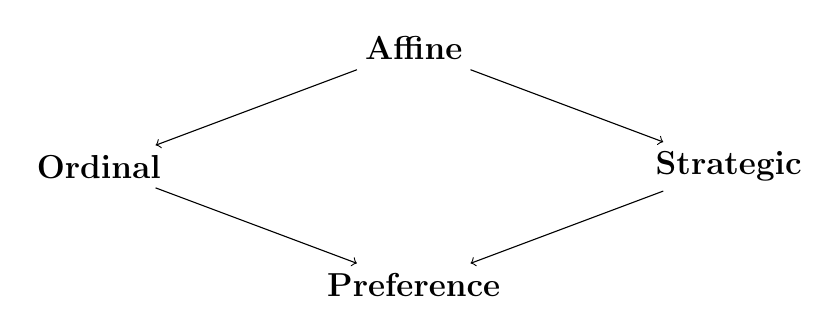
\begin{tikzpicture}
    %\node (Sc) at (0,10) {\textbf{Scaling}};
    \node (A) at (0,4) {\large\textbf{Affine}};
    \node (Str) at (4,2.5) {\large\textbf{Strategic}};
    \node (O) at (-4,2.5) {\large\textbf{Ordinal}};
    \node (P) at (0,1) {\large\textbf{Preference}};
    %\draw[->] (Sc) to (A);
    \draw[->] (A) to (Str);
    \draw[->] (A) to (O);
    \draw[->] (O) to (P);
    \draw[->] (Str) to (P);
    \end{tikzpicture}
\end{document}
\subsection{{Local boundedness and Lipschitz  properties of $\ell_{in}$, $\ell_{out}$, and their derivatives }}

\begin{proposition}[{Local} boundedness]\label{prop:uniform_boundedness}
Under \cref{assump:compact,assump:convexity_lin,assump:K_bounded,assump:reg_lin_lout}, the functions $(\omega,x,y)\mapsto \ell_{out}(\omega,h_{\omega}^{\star}(x),y)$, $(\omega,x,y)\mapsto \partial_{\omega}\ell_{out}(\omega,h_{\omega}^{\star}(x),y)$, and $(\omega,x,y)\mapsto\partial_v \ell_{out}(\omega, h^\star_\omega(x), y)$ are bounded over $\textnormal{hull}(\Omega)\times\mathcal{X}\times\mathcal{Y}$ by some positive constant $M_{out}$. Similarly, the functions $(\omega,x,y)\mapsto\partial_v \ell_{in}(\omega, h^\star_\omega(x), y)$, $(\omega,x,y)\mapsto\partial_v^2 \ell_{in}(\omega, h^\star_\omega(x), y)$, and $(\omega,x,y)\mapsto\partial_{\omega, v}^2 \ell_{in}(\omega, h^\star_\omega(x), y)$  are bounded over $\textnormal{hull}(\Omega)\times\mathcal{X}\times\mathcal{Y}$ by some positive constant $M_{in}$. 
The constants $M_{out}$ and $M_{in}$ are defined as:
\begin{align*}
M_{out}&\coloneqq\sup_{\omega\in\textnormal{hull}(\Omega),v\in\mathcal{V},y\in\mathcal{Y}}\max\left(\verts{\ell_{out}(\omega,v,y)},\Verts{\partial_{\omega}\ell_{out}(\omega,v,y)},\verts{\partial_v\ell_{out}(\omega, v, y)}\right)>0,\\
M_{in}&\coloneqq\sup_{\omega\in\textnormal{hull}(\Omega),v\in\mathcal{V},y\in\mathcal{Y}}\max\left(\verts{\partial_v\ell_{in}(\omega, v, y)}, \verts{\partial_v^2\ell_{in}(\omega, v, y)},\Verts{\partial_{\omega, v}^2\ell_{in}(\omega, v, y)}\right)>0,
\end{align*}
where $\mathcal{V}\subset\mathbb{R}$ is the compact interval defined in \cref{prop:bound_hstaromega}.
\end{proposition}

\begin{proof}
By \cref{prop:bound_hstaromega}, we have that $h^\star_\omega(x)\in\mathcal{V}\coloneqq\left[-\frac{B\kappa}{\lambda},\frac{B\kappa}{\lambda}\right]\subset\mathbb{R}$, for any $x\in\mathcal{X}$. From \cref{assump:reg_lin_lout}, we know that $\ell_{in}$, $\ell_{out}$, and their partial derivatives are all continuous on $\text{hull}(\Omega)\times\mathcal{V}\times\mathcal{Y}$. Also, $\mathcal{Y}$ is compact by \cref{assump:compact}. Thus, $\text{hull}(\Omega)\times\mathcal{V}\times\mathcal{Y}$ is compact. As every continuous function defined over a compact space is bounded, we obtain that:
\begin{align*}
    \sup_{\omega\in\text{hull}(\Omega),x\in\mathcal{X},y\in\mathcal{Y}}\verts{\ell_{out}(\omega,h_{\omega}^{\star}(x),y)}&\leq\sup_{\omega\in\text{hull}(\Omega),v\in\mathcal{V},y\in\mathcal{Y}}\verts{\ell_{out}(\omega,v,y)}<+\infty,\\
    \sup_{\omega\in\text{hull}(\Omega),x\in\mathcal{X},y\in\mathcal{Y}}\Verts{\partial_{\bullet} \ell_{\circ}(\omega,h_{\omega}^{\star}(x),y)}&\leq\sup_{\omega\in\text{hull}(\Omega),v\in\mathcal{V},y\in\mathcal{Y}}\Verts{\partial_{\bullet} \ell_{\circ}(\omega,v,y)}<+\infty,
\end{align*}
where $\bullet \in \{\{v\}, \{w\}, \{w,v\}\}$ and $\circ \in \{in,out\}$. This implies the desired result.
\end{proof}

\begin{proposition}[Local Lipschitz continuity]\label{prop:uniform_Lipschitzness}
	Under \cref{assump:compact,assump:convexity_lin,assump:K_bounded,assump:reg_lin_lout}, there exists a positive constant $\lipout$ so that for any $(x,y)$ in $\mathcal{X}\times \mathcal{Y}$, 
	the functions $\omega\mapsto \ell_{out}(\omega,h_{\omega}^{\star}(x),y)$, $\omega\mapsto \partial_{\omega}\ell_{out}(\omega,h_{\omega}^{\star}(x),y)$, and $\omega\mapsto\partial_v \ell_{out}(\omega, h^\star_\omega(x), y)$ are locally $\frac{\lipout}{\lambda}$-Lipschitz continuous over $\textnormal{hull}(\Omega)$. Similarly, there exists a positive constant $\lipin$ so that for any $(x,y)$ in $\mathcal{X}\times \mathcal{Y}$, the functions $\omega\mapsto\partial_v \ell_{in}(\omega, h^\star_\omega(x), y)$, $\omega\mapsto\partial_v^2 \ell_{in}(\omega, h^\star_\omega(x), y)$, and $\omega\mapsto\partial_{\omega, v}^2 \ell_{in}(\omega, h^\star_\omega(x), y)$ are locally $\frac{\lipin}{\lambda}$-Lipschitz continuous $\textnormal{hull}(\Omega)$.  The constants $\lipout$ and $\lipin$ are defined, for any $0<\lambda\leq \Lambda$, as:
	\begin{align*}
	    \lipout&\coloneqq\left(\Lambda+M_{in}\kappa\right)\max\left(M_{out},\bar{M}_{out}\right)>0\\
	    \lipin&\coloneqq\left(\Lambda+M_{in}\kappa\right)\max\left(M_{in},\bar{M}_{in}\right)>0,
    \end{align*}
    where:
    \begin{align*}
      \bar{M}_{out}&\coloneqq\sup_{\omega\in\textnormal{hull}(\Omega), v\in\mathcal{V}, y\in\mathcal{Y}}\max\left(\Verts{\partial_\omega^2\ell_{out}(\omega, v, y)}_{\op},\Verts{\partial_{\omega, v}^2\ell_{out}(\omega, v, y)},\verts{\partial_v^2\ell_{out}(\omega, v, y)}\right)>0,\\
      \bar{M}_{in}&\coloneqq\sup_{\omega\in\textnormal{hull}(\Omega), v\in\mathcal{V}, y\in\mathcal{Y}}\max\left(\Verts{\partial_\omega\partial_v^2\ell_{in}(\omega, v, y)},\verts{\partial_v^3\ell_{in}(\omega, v, y)},\Verts{\partial_\omega\partial_{\omega, v}^2\ell_{in}(\omega, v, y)}\right)>0,
    \end{align*}
    with $M_{in}$ and $M_{out}$ being the positive constants defined in \cref{prop:uniform_boundedness}, and $\mathcal{V}\subset\mathbb{R}$ is the compact interval defined in \cref{prop:bound_hstaromega}.
\end{proposition}


\begin{proof}
For any $(\omega,x,y)\in\text{hull}(\Omega)\times \mathcal{X}\times \mathcal{Y}$, we have:
\begin{align*}
    \Verts{\nabla_\omega\ell_{out}(\omega, h^\star_\omega(x), y)}&=\Verts{\partial_\omega\ell_{out}(\omega, h^\star_\omega(x), y)+\partial_v\ell_{out}(\omega, h^\star_\omega(x), y)\partial_\omega h^\star_\omega(x)}\\
    &\leq\Verts{\partial_\omega\ell_{out}(\omega, h^\star_\omega(x), y)}+\verts{\partial_v\ell_{out}(\omega, h^\star_\omega(x), y)}\Verts{\partial_\omega h^\star_\omega}_{\op}\Verts{K(x,\cdot)}_\mathcal{H}\\
    &\leq M_{out}\left(1+\frac{M_{in}\kappa}{\lambda}\right)\\
    &\leq\frac{M_{out}\left(\Lambda+M_{in}\kappa\right)}{\lambda},
\end{align*}
where the first line uses the chain rule, the second line applies the triangle inequality and the reproducing property of the RKHS $\mathcal{H}$, the third line follows from \cref{prop:uniform_boundedness} to bound the derivatives of $\ell_{out}$, from \cref{prop:lip_hstaromega}, which states that the function $\omega\mapsto h^\star_\omega$ is $\frac{L\sqrt{\kappa}}{\lambda}$-Lipschitz continuous with $L\coloneqq\sup_{\omega\in\text{hull}(\Omega),v\in\mathcal{V},y\in\mathcal{Y}}\left\|\partial_{\omega, v}^2 \ell_{in}(\omega, v, y)\right\|<M_{in}$, to bound $\Verts{\partial_\omega h^\star_\omega}_{\op}$, and from \cref{assump:K_bounded} to bound $\Verts{K(x,\cdot)}_\mathcal{H}$, and the last line is a direct consequence of $0<\lambda\leq \Lambda$. In a similar way, we obtain:
\begin{gather*}
    \Verts{\nabla_\omega\partial_\omega\ell_{out}(\omega, h^\star_\omega(x), y)}_{\op}\leq\frac{\bar{M}_{out}\left(\Lambda+M_{in}\kappa\right)}{\lambda},\quad\Verts{\nabla_\omega\partial_v \ell_{out}(\omega, h^\star_\omega(x), y)}\leq\frac{\bar{M}_{out}\left(\Lambda+M_{in}\kappa\right)}{\lambda},\\
    \Verts{\nabla_\omega\partial_v \ell_{in}(\omega, h^\star_\omega(x), y)}\leq\frac{M_{in}\left(\Lambda+M_{in}\kappa\right)}{\lambda},\quad\Verts{\nabla_\omega\partial_v^2 \ell_{in}(\omega, h^\star_\omega(x), y)}\leq\frac{\bar{M}_{in}\left(\Lambda+M_{in}\kappa\right)}{\lambda},\\
    \Verts{\nabla_\omega\partial_{\omega, v}^2 \ell_{in}(\omega, h^\star_\omega(x), y)}_{\op}\leq\frac{\bar{M}_{in}\left(\Lambda+M_{in}\kappa\right)}{\lambda}.
\end{gather*}
Combining all these bounds concludes the proof.
\end{proof}

\section{Generalization Properties}\label{app:sec_conv}

{As before, let $\Omega$ be an arbitrary compact subset of $\mathbb{R}^d$.}

\subsection{Point-wise estimates}\label{app:subsec_point_est}
We present a point-wise upper-bound on the value error $\verts{\mathcal{F}(\omega)-\widehat{\mathcal{F}}(\omega) }$ and gradient error $\Verts{\nabla\mathcal{F}(\omega)-\widehat{\nabla\mathcal{F}}(\omega) }$. To this end, we introduce the following notation for the error between the inner and outer objectives and their empirical approximations evaluated at the optimal inner solution $h_{\omega}^{\star}$: 
\begin{align*}
    \Dout\coloneqq \verts{L_{out}(\omega, h^\star_\omega)-\widehat{L}_{out}(\omega, h^\star_\omega)}, 
    \qquad 
    \Din \coloneqq \verts{L_{in}(\omega, h^\star_\omega)-\widehat{L}_{in}(\omega, h^\star_\omega)}.
\end{align*}
By abuse of notation, we introduce the following error between  partial derivatives of $L_{in}$ and $\widehat{L}_{in}$ (resp. $L_{out}$ and $\widehat{L}_{out}$), evaluated at $(\omega, h_{\omega}^{\star})$, \textit{i.e.},
\begin{align*}
  \Douth &\coloneqq \Verts{\partial_h L_{out}(\omega, h^\star_\omega)-\partial_h\widehat{L}_{out}(\omega, h^\star_\omega)}_{\mathcal{H}},\quad 
  &\Doutw &\coloneqq \Verts{\partial_\omega L_{out}(\omega, h^\star_\omega)-\partial_\omega\widehat{L}_{out}(\omega, h^\star_\omega)},\\
  \Dinh &\coloneqq \Verts{\partial_h L_{in}(\omega, h^\star_\omega)-\partial_h\widehat{L}_{in}(\omega, h^\star_\omega)}_{\mathcal{H}},\quad 
  &\Dinw &\coloneqq \Verts{\partial_\omega L_{in}(\omega, h^\star_\omega)-\partial_\omega\widehat{L}_{in}(\omega, h^\star_\omega)},\\
  \Dinhh &\coloneqq \Verts{\partial_{h}^2 L_{in}(\omega, h^\star_\omega)-\partial_h^2\widehat{L}_{in}(\omega, h^\star_\omega)}_{\op},\quad 
  &\Dinwh &\coloneqq \Verts{\partial_{\omega,h}^2 L_{in}(\omega, h^\star_\omega)-\partial_{\omega,h}^2\widehat{L}_{in}(\omega, h^\star_\omega)}_{\op}.
\end{align*}

\begin{proposition}\label{prop:diff_hstar_hhat}
    Under \cref{assump:compact,assump:convexity_lin,assump:K_bounded,assump:reg_lin_lout}, the following holds for any $\omega\in\Omega$:
    \begin{equation*}
        \left\|h^\star_\omega-\hat{h}_\omega\right\|_\mathcal{H}\leq\frac{1}{\lambda}\left\| \partial_h\widehat{L}_{in}(\omega, h^\star_\omega)\right\|_\mathcal{H} = \frac{1}{\lambda}\Dinh.
    \end{equation*}
\end{proposition}
\begin{proof}
Let $\omega\in\Omega$. 
The function $h\mapsto\widehat{L}_{in}(\omega, h)$ is $\lambda$-strongly convex and Fr\'echet differentiable by  \cref{prop:strong_convexity_Lin,prop:fre_diff_L}. Moreover,  $\hat{h}_{\omega}$ is the minimizer of $h\mapsto\widehat{L}_{in}(\omega, h)$ by definition. 
Therefore, using \cref{lem:h_min_hstar}, we obtain a control on the distance in $\mathcal{H}$ to the optimum $\hat{h}_{\omega}$ of $h\mapsto\widehat{L}_{in}(\omega,h)$ in terms of the gradient $\partial_{h}\widehat{L}_{in}(\omega,h)$:
\begin{align*}
	\left\|h-\hat{h}_\omega\right\|_\mathcal{H}\leq\frac{1}{\lambda}\Verts{\partial_h\widehat{L}_{in}(\omega, h)}_\mathcal{H}, \qquad \forall h\in \mathcal{H}.
\end{align*}
In particular, choosing $h= h^\star_\omega$ yields the first inequality. The fact that $\Verts{\partial_h\widehat{L}_{in}(\omega, h_{\omega}^{\star})}_\mathcal{H}=\Dinh$ follows from the optimality of $h_{\omega}^{\star}$ which implies that  $\partial_h L_{in}(\omega, h_{\omega}^{\star})=0$. 
\end{proof}

\begin{proposition}\label{prop:lip_continuity_out}
Under \cref{assump:compact,assump:convexity_lin,assump:K_bounded,assump:reg_lin_lout}, the following inequalities hold for any $\omega\in\Omega$:
\begin{align*}
	\Eout &\coloneqq\verts{\widehat{L}_{out}(\omega, h^\star_\omega)-\widehat{L}_{out}(\omega, \hat{h}_\omega)}\leq C_{out}\Verts{h^\star_\omega-\hat{h}_\omega}_\mathcal{H},\\
	\Eouth&\coloneqq\Verts{\partial_h\widehat{L}_{out}(\omega, h^\star_\omega)-\partial_h\widehat{L}_{out}(\omega, \hat{h}_\omega)}_\mathcal{H} \leq C_{out}\Verts{h^\star_\omega-\hat{h}_\omega}_\mathcal{H},\\
	\Eoutw&\coloneqq\Verts{\partial_\omega\widehat{L}_{out}(\omega, h^\star_\omega)-\partial_\omega\widehat{L}_{out}(\omega, \hat{h}_\omega)} \leq C_{out}\Verts{h^\star_\omega-\hat{h}_\omega}_\mathcal{H},\\
	\Einhh&\coloneqq\Verts{\partial_h^2\widehat{L}_{in}(\omega, h^\star_\omega)-\partial_h^2\widehat{L}_{in}(\omega, \hat{h}_\omega)}_{\op}\leq C_{in}\Verts{h^\star_\omega-\hat{h}_\omega}_\mathcal{H},\\
	\Einwh&\coloneqq\Verts{\partial_{\omega, h}^2\widehat{L}_{in}(\omega, h^\star_\omega)-\partial_{\omega, h}^2\widehat{L}_{in}(\omega, \hat{h}_\omega)}_{\op} \leq C_{in}\Verts{h^\star_\omega-\hat{h}_\omega}_\mathcal{H}.
\end{align*}
The positive constants $C_{out}$ and $C_{in}$ are defined as:
\begin{align*}
    C_{out}&\coloneqq\max\left(M_{out}\sqrt{\kappa},\bar{M}_{out}\kappa,\bar{M}_{out}\sqrt{\kappa}\right)>0,\\
    C_{in}&\coloneqq\max\left(\bar{M}_{in}\kappa\sqrt{\kappa},\bar{M}_{in}\kappa,M_{in}\sqrt{d\kappa}\right)>0,
\end{align*}
where $M_{out}$, $\bar{M}_{out}$, and $\bar{M}_{in}$ are the positive constants defined in \cref{prop:uniform_boundedness,prop:uniform_Lipschitzness}.
\end{proposition}

\begin{proof}
\textbf{Lipschitz continuity of some functions of interest. }Let $\omega\in\Omega$. According to \cref{prop:bound_hstaromega}, both $h^\star_\omega(x)$ and $\hat{h}_\omega(x)$ lie in the compact interval $\mathcal{V}\coloneqq\left[-\frac{B\kappa}{\lambda},\frac{B\kappa}{\lambda}\right]\subset\mathbb{R}$, for any $x\in\mathcal{X}$, where $B\coloneqq\sup_{\omega\in\text{hull}(\Omega),y\in\mathcal{Y}}\left|\partial_v \ell_{in}(\omega, 0, y)\right|>0$. By \cref{assump:compact}, $\mathcal{Y}$ is a compact set. Hence $\Omega\times\mathcal{V}\times\mathcal{Y}$ is a compact set as well. Furthermore, by \cref{assump:reg_lin_lout}, $(\omega, v, y)\mapsto\ell_{in}(\omega, v, y)$, $(\omega, v, y)\mapsto\ell_{out}(\omega, v, y)$, and their derivatives are all continuous over the compact domain $\Omega\times\mathcal{V}\times\mathcal{Y}$. Therefore, these functions and their derivatives are bounded on this domain. In particular, this also holds when $v$ takes the specific values $h^\star_\omega(x)$ or $\hat{h}_\omega(x)$. Let $\bar{v}$ be either $h^\star_\omega(x)$ or $\hat{h}_\omega(x)$, for any $x\in\mathcal{X}$. For any $\omega\in\Omega$, and $y\in\mathcal{Y}$, we have:
\begin{align*}
    \verts{\partial_v\ell_{out}(\omega, \bar{v}, y)}&\leq\sup_{\omega\in\Omega,v\in\mathcal{V},y\in\mathcal{Y}}\verts{\partial_v\ell_{out}(\omega, v, y)}\leq M_{out}<+\infty,\\
   \verts{\partial_v^2\ell_{out}(\omega, \bar{v}, y)}&\leq\sup_{\omega\in\Omega,v\in\mathcal{V},y\in\mathcal{Y}}\verts{\partial_v^2\ell_{out}(\omega, v, y)}\leq\bar{M}_{out}<+\infty,\\
   \Verts{\partial_{\omega, v}^2\ell_{out}(\omega, \bar{v}, y)}&\leq\sup_{\omega\in\Omega,v\in\mathcal{V},y\in\mathcal{Y}}\Verts{\partial_{\omega, v}^2\ell_{out}(\omega, v, y)}\leq\bar{M}_{out}<+\infty,\\
   \verts{\partial_v^3\ell_{in}(\omega, \bar{v}, y)}&\leq\sup_{\omega\in\Omega,v\in\mathcal{V},y\in\mathcal{Y}}\verts{\partial_v^3\ell_{in}(\omega, v, y)}\leq\bar{M}_{in}<+\infty,\\
   \Verts{\partial_v\partial_{\omega, v}^2\ell_{in}(\omega, \bar{v}, y)}_{\op}&\leq\sup_{\omega\in\Omega,v\in\mathcal{V},y\in\mathcal{Y}}\Verts{\partial_\omega\partial_v^2\ell_{in}(\omega, v, y)}\leq\bar{M}_{in}<+\infty
\end{align*}
This means that $v\in\mathcal{V}\mapsto\ell_{out}(\omega, v, y)$, $v\in\mathcal{V}\mapsto\partial_v\ell_{out}(\omega, v, y)$, $v\in\mathcal{V}\mapsto\partial_\omega\ell_{out}(\omega, v, y)$, $v\in\mathcal{V}\mapsto\partial_v^2\ell_{in}(\omega, v, y)$, and $v\in\mathcal{V}\mapsto\partial_{\omega, v}^2\ell_{in}(\omega, v, y)$ are Lipschitz continuous, with Lipschitz constants $M_{out}$, $\bar{M}_{out}$, $\bar{M}_{out}$, $\bar{M}_{in}$, and $\bar{M}_{in}$, respectively, for any $\omega\in\Omega$ and $y\in\mathcal{Y}$.

\textbf{Upper-bounds. }We have:
\begin{align*}
    \Eout\coloneqq\verts{\widehat{L}_{out}(\omega, h^\star_\omega)-\widehat{L}_{out}(\omega, \hat{h}_\omega)}&=\verts{\frac{1}{m}\sum_{j=1}^m\ell_{out}(\omega, h^\star_\omega(\tilde{x}_j), \tilde{y}_j) - \frac{1}{m}\sum_{j=1}^m\ell_{out}(\omega, \hat{h}_\omega(\tilde{x}_j), \tilde{y}_j)}\\
    &\leq\frac{1}{m}\sum_{j=1}^m\verts{\ell_{out}(\omega, h^\star_\omega(\tilde{x}_j), \tilde{y}_j)-\ell_{out}(\omega, \hat{h}_\omega(\tilde{x}_j), \tilde{y}_j)}\\
    &\leq\frac{M_{out}}{m}\sum_{j=1}^m\verts{h^\star_\omega(\tilde{x}_j)-\hat{h}_\omega(\tilde{x}_j)}\\
    &\leq M_{out}\sqrt{\kappa}\Verts{h^\star_\omega-\hat{h}_\omega}_\mathcal{H},
\end{align*}
where the first line uses the definition of $(\omega, h)\mapsto\widehat{L}_{out}(\omega, h)$, the second line applies the triangle inequality, the third line leverages the fact that $v\mapsto\ell_{out}(\omega, v, y)$ is $M_{out}$-Lipschitz continuous, for any $\omega\in\Omega$ and $y\in\mathcal{Y}$, and the last line follows from the reproducing property of the RKHS $\mathcal{H}$, Cauchy-Schwarz's inequality, and \cref{assump:K_bounded} to bound $\Verts{K(x,\cdot)}_\mathcal{H}$ by $\sqrt{\kappa}$. Similarly, we obtain:
\begin{gather*}
    \partial_h\Eout\leq\bar{M}_{out}\kappa\Verts{h^\star_\omega-\hat{h}_\omega}_\mathcal{H},\quad\partial_\omega\Eout\leq\bar{M}_{out} \sqrt{\kappa}\Verts{h^\star_\omega-\hat{h}_\omega}_\mathcal{H},\quad\partial_h^2\Ein\leq\bar{M}_{in} \kappa\sqrt{\kappa}\Verts{h^\star_\omega-\hat{h}_\omega}_\mathcal{H},\\
    \partial_{\omega, h}^2\Ein\leq\bar{M}_{in} \kappa\Verts{h^\star_\omega-\hat{h}_\omega}_\mathcal{H}.
\end{gather*}
Combining all the bounds finishes the proof.
\end{proof}

\begin{proposition}\label{prop:bounded_derivatives}
Under \cref{assump:compact,assump:convexity_lin,assump:K_bounded,assump:reg_lin_lout}, the following inequalities hold for any $\omega\in\Omega$:
\begin{align*}
	\Verts{\partial_{h}L_{out}(\omega,h_{\omega}^{\star})}_{\mathcal{H}}\leq C_{out}, \quad \Verts{\partial^2_{\omega,h}L_{in}(\omega,h_{\omega}^{\star}) }_{\op}\leq C_{in},\quad 
	\Verts{\partial^2_{\omega,h}\widehat{L}_{in}(\omega,\hat{h}_{\omega}) }_{\op}\leq C_{in},
\end{align*}
where $C_{out}$ and $C_{in}$ are the positive constants defined in \cref{prop:lip_continuity_out}.
\end{proposition}

\begin{proof}Let $\omega\in\Omega$.

\textbf{Upper-bound on $\Verts{\partial_{h}L_{out}(\omega,h_{\omega}^{\star})}_{\mathcal{H}}$. }We have:
\begin{align*}
    \left\|\partial_h L_{out}(\omega, h^\star_\omega)\right\|_\mathcal{H}&=\Big\|\mathbb{E}_\mathbb{Q}\left[\partial_v \ell_{out}(\omega, h^\star_\omega(x), y)K(x,\cdot)\right]\Big\|_\mathcal{H}\\
    &\leq\mathbb{E}_\mathbb{Q}\Big[\left|\partial_v \ell_{out}(\omega, h^\star_\omega(x), y)\right|\left\|K(x,\cdot)\right\|_\mathcal{H}\Big]\\
    &\leq\sqrt{\kappa}\mathbb{E}_\mathbb{Q}\Big[\left|\partial_v \ell_{out}(\omega, h^\star_\omega(x), y)\right|\Big],
\end{align*}
where the first line follows from \cref{prop:fre_diff_L}, the second line results from the triangle inequality, and the last line uses \cref{assump:K_bounded} to bound $\Verts{K(x,\cdot)}_\mathcal{H}$ by $\sqrt{\kappa}$.  Furthermore, we know by \cref{prop:bound_hstaromega} that $(\omega,h_{\omega}^{\star}(x),y)$ belongs to the compact subset $\Omega\times \mathcal{V}\times \mathcal{Y}$ and by \cref{prop:uniform_boundedness} that $\partial_v \ell_{out}(\omega, h^\star_\omega(x), y)$ is bounded by a  constant $M_{out}$ on $\text{hull}(\Omega)\times \mathcal{V}\times \mathcal{Y}$. Hence, it follows that:
\begin{align*}
    \left\|\partial_h L_{out}(\omega, h^\star_\omega)\right\|_\mathcal{H}
    \leq \sqrt{\kappa} M_{out} \le C_{out},
\end{align*}
where $C_{out}$ is defined in \cref{prop:lip_continuity_out}. 

\textbf{Upper-boud on $\quad \Verts{\partial^2_{\omega,h}L_{in}(\omega,h_{\omega}^{\star}) }_{\op}$. }According to \cref{prop:fre_diff_L_v}, $\partial_{\omega, h}^2 L_{in}(\omega, h^\star_\omega)$ is a Hilbert-Schmidt operator, which points to:
\begin{equation}\label{eq:norm_op_partial_omega_h_Lin}
    \left\|\partial_{\omega, h}^2L_{in}(\omega, h^\star_\omega)\right\|_{\op}\leq\left\|\partial_{\omega, h}^2L_{in}(\omega, h^\star_\omega)\right\|_{\hs}=\sqrt{\sum_{l=1}^d\left\|\partial_{\omega_k, h}^2L_{in}(\omega, h^\star_\omega)\right\|_\mathcal{H}^2}.
\end{equation}
This means that to find an upper-bound on $\left\|\partial_{\omega, h}^2L_{in}(\omega, h^\star_\omega)\right\|_{\op}$, it suffices to establish an upper-bound on $\left\|\partial_{\omega_l, h}^2L_{in}(\omega, h^\star_\omega)\right\|_\mathcal{H}^2$ for any $l\in\{1,\ldots,d\}$. For a fixed $l\in\{1,\ldots,d\}$, we have:
\begin{align*}
    \left\|\partial_{\omega_l, h}^2L_{in}(\omega, h^\star_\omega)\right\|_\mathcal{H}^2&=\Big\|\mathbb{E}_\mathbb{P}\left[\partial_{\omega_l,v}^2 \ell_{in}(\omega, h^\star_\omega(x), y)K(x,\cdot)\right]\Big\|_\mathcal{H}^2\\
    &\leq\mathbb{E}_\mathbb{P}\left[\left|\partial_{\omega_l, v}^2 \ell_{in}(\omega, h^\star_\omega(x), y)\right|^2\left\|K(x,\cdot)\right\|_\mathcal{H}^2\right]\\
    &\leq\mathbb{E}_\mathbb{P}\left[\left\|\partial_{\omega, v}^2 \ell_{in}(\omega, h^\star_\omega(x), y)\right\|^2\right]\kappa,
\end{align*}
where the first line follows from \cref{prop:fre_diff_L_v}, the second line is a consequence of Jensen's inequality applied on the convex function $\|\cdot\|^2$, and the last line applies \cref{assump:K_bounded} to bound $\Verts{K(x,\cdot)}_\mathcal{H}^2$ by $\kappa$. Incorporating this upper-bound into \cref{eq:norm_op_partial_omega_h_Lin} yields:
\begin{equation*}
    \left\|\partial_{\omega, h}^2L_{in}(\omega, h^\star_\omega)\right\|_{\op}\leq\sqrt{\mathbb{E}_\mathbb{P}\left[\left\|\partial_{\omega, v}^2 \ell_{in}(\omega, h^\star_\omega(x), y)\right\|^2\right] d\kappa}\leq M_{in}\sqrt{d\kappa}\leq C_{out}, 
\end{equation*}
where we used \cref{prop:uniform_boundedness} to bound $\partial_{\omega, v}^2 \ell_{in}(\omega, h^\star_\omega(x), y)$ by the constant $M_{in}$.

\textbf{Upper-bound on $\Verts{\partial^2_{\omega,h}\widehat{L}_{in}(\omega,\hat{h}_{\omega}) }_{\op}$. }The derivation of this upper bound follows the same steps as the previous one, with the only differences being the use of $\widehat{L}_{in}$ instead of $L_{in}$, and $\hat{h}_\omega$ instead of $h^\star_\omega$.

Note that in the last step of each of the three upper-bounds, we used the fact that the functions we are dealing with are continuous (by \cref{assump:reg_lin_lout}) on $\Omega\times\mathcal{V}\times\mathcal{Y}$, which is compact because $\Omega$ and $\mathcal{Y}$ are compact by \cref{assump:compact} and $\mathcal{V}$ is a compact interval of $\mathbb{R}$ defined in \cref{prop:bound_hstaromega}. Hence, those functions are bounded.
\end{proof}


\begin{proposition}[{Approximation bounds}]\label{prop:grad_app_bound}
    Under \cref{assump:compact,assump:convexity_lin,assump:K_bounded,assump:reg_lin_lout}, the following holds for any $\omega\in\Omega$:
    \begin{gather*}
    \verts{\mathcal{F}(\omega)-\widehat{\mathcal{F}}(\omega)}\leq 
    \Dout
    +\frac{C_{out}}{\lambda}\Dinh,\\
 	\Verts{\nabla\mathcal{F}(\omega)-\widehat{\nabla\mathcal{F}}(\omega)}
 	\leq  
 	\Doutw  + \frac{C_{in}}{\lambda}\Douth + \frac{C_{out}C_{in}}{\lambda^2}\Dinhh + \frac{C_{out}}{\lambda}\Dinwh + \frac{C_{out}}{\lambda}\parens{1 + 2\frac{C_{in}}{\lambda}  + \frac{C_{in}^2}{\lambda^2} }\Dinh,
    \end{gather*}
 where the constants $C_{in}$ and $C_{out}$ are given in {\cref{prop:lip_continuity_out}}.
\end{proposition}
\begin{proof}
In all what follows, we fix a value for $\omega$ in $\Omega$. We start by controlling the value function, then its gradient.

{\bf Control on the value function.}
By the triangle inequality, we have:
\begin{equation}\label{eq:diff_f_int}
    \verts{\mathcal{F}(\omega)-\hat{\mathcal{F}}(\omega)}\leq\underbrace{\verts{L_{out}(\omega, h^\star_\omega)-\widehat{L}_{out}(\omega, h^\star_\omega)}}_{\delta_{\omega}^{out}} +\underbrace{\verts{\widehat{L}_{out}(\omega, h^\star_\omega)-\widehat{L}_{out}(\omega, \hat{h}_\omega)}}_{\Eout},
\end{equation}
According to \cref{prop:lip_continuity_out}, the error term $\Eout$ is controlled by the norm of the difference $h^\star_\omega-\hat{h}_\omega$, \textit{i.e.}, $\Eout\leq C_{out}\Verts{h^\star_\omega-\hat{h}_\omega}_\mathcal{H}$. 
Moreover, by \cref{prop:diff_hstar_hhat}, we know that $\Verts{h^\star_\omega-\hat{h}_\omega}_\mathcal{H}\leq \frac{1}{\lambda}\Dinh$. Therefore, combining both bounds yields: 
	$\Eout\leq \frac{C_{out}}{\lambda}\Dinh$. 
The upper-bound on value function follows by substituting the previous inequality into \cref{eq:diff_f_int}. 

{\bf Control on the gradient.}
By \cref{prop:tot_grad_int}, we have the following expression for the total gradient $\nabla\mathcal{F}$:
\begin{align*}
    \nabla\mathcal{F}(\omega)=\partial_\omega L_{out}(\omega, h^\star_\omega)-\partial_{\omega, h}^2 L_{in}(\omega, h^\star_\omega)\left(\partial_h^2 L_{in}(\omega, h^\star_\omega)\right)^{-1}\partial_h L_{out}(\omega, h^\star_\omega).
\end{align*}
{Similarly, the gradient estimator $\widehat{\nabla\mathcal{F}}$ is defined by replacing $L_{out}$ and $L_{in}$ by their empirical versions $\widehat{L}_{out}$ and $\widehat{L}_{in}$, and $h_{\omega}^{\star}$ by $\hat{h}_{\omega}\coloneqq\arg\min_{h\in \mathcal{H}} \widehat{L}_{in}(\omega,h)$ in the above expression, \textit{i.e.},}
\begin{align*}
    \widehat{\nabla\mathcal{F}}(\omega)=\partial_\omega\widehat{L}_{out}(\omega, \hat{h}_\omega)-\partial_{\omega, h}^2 \widehat{L}_{in}(\omega, \hat{h}_\omega)\left(\partial_h^2 \widehat{L}_{in}(\omega, \hat{h}_\omega)\right)^{-1}\partial_h \widehat{L}_{out}(\omega, \hat{h}_\omega).
\end{align*}
To simplify notations, for any $h\in\mathcal{H}$, we introduce the following operators $R(h), \hat{R}(h):\mathcal{H}\to\Omega$:    \begin{align*}
        R(h)=\partial_{\omega, h}^2L_{in}(\omega, h)\left(\partial_h^2 L_{in}(\omega, h)\right)^{-1}\quad\text{and}\quad 
        \hat{R}(h)=\partial_{\omega, h}^2\widehat{L}_{in}(\omega, h)\left(\partial_h^2 \widehat{L}_{in}(\omega, h)\right)^{-1}.
    \end{align*}
    The difference $\nabla\mathcal{F}(\omega)-\widehat{\nabla\mathcal{F}}(\omega)$ can be decomposed as:
    \begin{align*}
        \nabla\mathcal{F}(\omega)-\widehat{\nabla\mathcal{F}}(\omega)=&\left(\partial_\omega L_{out}(\omega,h^\star_\omega)-\partial_\omega \widehat{L}_{out}(\omega,h^\star_\omega)\right)+\left(\partial_\omega \widehat{L}_{out}(\omega,h^\star_\omega)-\partial_\omega \widehat{L}_{out}(\omega,\hat{h}_\omega)\right)\\
        &-\hat{R}(\hat{h}_\omega)\parens{\left(\partial_h L_{out}(\omega,h^\star_\omega)-\partial_h\widehat{L}_{out}(\omega,h^\star_\omega)\right)+ \left(\partial_h\widehat{L}_{out}(\omega,h^\star_\omega)-\partial_h\widehat{L}_{out}(\omega,\hat{h}_\omega)\right)}\\
                &-\left(R(h^\star_\omega)-\hat{R}(\hat{h}_\omega)\right)\partial_h L_{out}(\omega,h^\star_\omega).
    \end{align*}
By taking the norm of the above equality and using triangle inequality, we obtain the following upper-bound: 
    \begin{align}
    \begin{split}
        \Verts{\nabla\mathcal{F}(\omega)-\widehat{\nabla\mathcal{F}}(\omega)}
        & \leq
        \underbrace{\Verts{\partial_\omega L_{out}(\omega,h^\star_\omega)-\partial_\omega \widehat{L}_{out}(\omega,h^\star_\omega)}}_{\Doutw}+\underbrace{\Verts{\partial_\omega \widehat{L}_{out}(\omega,h^\star_\omega)-\partial_\omega \widehat{L}_{out}(\omega,\hat{h}_\omega)}}_{\Eoutw}\\
        +&\Verts{\hat{R}(\hat{h}_{\omega})}_{\op}\parens{\underbrace{\Verts{\partial_h L_{out}(\omega,h^\star_\omega)-\partial_h\widehat{L}_{out}(\omega,h^\star_\omega)}_{\mathcal{H}}}_{\Douth} + \underbrace{\Verts{\partial_h\widehat{L}_{out}(\omega,h^\star_\omega)-\partial_h\widehat{L}_{out}(\omega,\hat{h}_\omega)}_{\mathcal{H}}}_{\Eouth}}\\
                +& \Verts{R(h^\star_\omega)-\hat{R}(\hat{h}_\omega)}_{\op}\Verts{\partial_h L_{out}(\omega,h^\star_\omega)}_{\mathcal{H}}.
                \end{split}\label{eq:diff_grad_inter}
    \end{align}
    Next, we provide upper-bounds on $\Verts{R(h_{\omega}^{\star})- \hat{R}(\hat{h}_{\omega})}_{\op}$ and $\Verts{\hat{R}(\hat{h}_{\omega})}_{\op}$ in terms of derivatives of $L_{in}$ and $\widehat{L}_{in}$. 

    \textbf{Upper-bounds on $\Verts{R(h_{\omega}^{\star})- \hat{R}(\hat{h}_{\omega})}_{\op}$ and $\Verts{\hat{R}(\hat{h}_{\omega})}_{\op}$. } 
    %
    By application of {\cref{prop:fre_diff_L_v,prop:strong_convexity_Lin}}, we deduce that $\partial_{\omega,h}^2 L_{in}(\omega,h_{\omega}^{\star})$, $\partial_{h}^2 L_{in}(\omega,h_{\omega}^{\star})$, $\partial_{\omega,h}^2 \widehat{L}_{in}(\omega,\hat{h}_{\omega})$ and $\partial_{h}^2 \widehat{L}_{in}(\omega,\hat{h}_{\omega})$ are all bounded operators. Moreover, since $L_{in}$ and $\widehat{L}_{in}$ are $\lambda$-strongly  convex in their second argument by {\cref{prop:strong_convexity_Lin}}, it follows that $\partial_{h}^2 L_{in}(\omega,h_{\omega}^{\star})\geq \lambda\Id_{\mathcal{H}}$ and $\partial_{h}^2 \widehat{L}_{in}(\omega,\hat{h}_{\omega})\geq \lambda \Id_{\mathcal{H}}$. We can therefore apply \cref{lem:tech_res_1} which yields the following inequalities:  
    \begin{align*}
        \Verts{R(h_{\omega}^{\star})- \hat{R}(\hat{h}_{\omega})}_{\op}
        \leq & \frac{1}{\lambda^2}\Verts{\partial_{\omega,h}^2 L_{in}(\omega,h_{\omega}^{\star})}_{\op}\Verts{\partial_{h}^2 L_{in}(\omega,h_{\omega}^{\star}) - \partial_{h}^2 \widehat{L}_{in}(\omega,\hat{h}_{\omega})}_{\op}\\ 
        &+ \frac{1}{\lambda}\Verts{\partial_{\omega,h}^2 L_{in}(\omega,h_{\omega}^{\star}) - \partial_{\omega,h}^2 \widehat{L}_{in}(\omega,\hat{h}_{\omega})}_{\op},\\
        \Verts{\hat{R}(\hat{h}_{\omega})}_{\op}\leq&\frac{1}{\lambda} \Verts{\partial_{\omega,h}^2\widehat{L}_{in}(\omega,\hat{h}_{\omega})}_{\op}. 
    \end{align*}
By applying the triangle inequality to both terms of the first inequality above, we obtain:
\begin{align*}
        \Verts{R(h_{\omega}^{\star})- \hat{R}(\hat{h}_{\omega})}_{\op}
        \leq & \frac{1}{\lambda^2}\Verts{\partial_{\omega,h}^2 L_{in}(\omega,h_{\omega}^{\star})}_{\op}\parens{\underbrace{\Verts{\partial_{h}^2 L_{in}(\omega,h_{\omega}^{\star}) - \partial_{h}^2 \widehat{L}_{in}(\omega,h^\star_{\omega})}_{\op}}_{\Dinhh} + \underbrace{\Verts{\partial_{h}^2 \widehat{L}_{in}(\omega,h_{\omega}^{\star}) - \partial_{h}^2 \widehat{L}_{in}(\omega,\hat{h}_{\omega})}_{\op}}_{\Einhh}}\\ 
        &+ \frac{1}{\lambda}\parens{\underbrace{\Verts{\partial_{\omega,h}^2 L_{in}(\omega,h_{\omega}^{\star}) - \partial_{\omega,h}^2 \widehat{L}_{in}(\omega,h_{\omega}^{\star})}_{\op}}_{\Dinwh} + \underbrace{\Verts{\partial_{\omega,h}^2 \widehat{L}_{in}(\omega,h_{\omega}^{\star}) - \partial_{\omega,h}^2 \widehat{L}_{in}(\omega,\hat{h}_{\omega})}_{\op}}_{\Einwh}}.
    \end{align*}
{\bf Final bound.} We can now substitute the above bounds on $\Verts{R(h_{\omega}^{\star})- \hat{R}(\hat{h}_{\omega})}_{\op}$ and $\Verts{\hat{R}(\hat{h}_{\omega})}_{\op}$ into \cref{eq:diff_grad_inter} to obtain the following upper-bound on the gradient error:
 \begin{equation} \label{eq:diff_grad_inter_2}
\begin{aligned}
 	\Verts{\nabla\mathcal{F}(\omega)-\widehat{\nabla\mathcal{F}}(\omega)}
 	&\leq  
 	\Doutw + \Eoutw + \frac{1}{\lambda}\Verts{\partial_{\omega,h}^2 \widehat{L}_{in}(\omega,\hat{h}_{\omega})}_{\op}\parens{\Douth + \Eouth}\\
 	+& \Verts{\partial_{h}L_{out}(\omega,h_{\omega}^{\star})}_{\mathcal{H}}\parens{ \frac{1}{\lambda^2}\Verts{\partial^2_{\omega,h}L_{in}(\omega,h_{\omega}^{\star}) }_{\op} \parens{\Dinhh + \Einhh} + \frac{1}{\lambda}\parens{\Dinwh + \Einwh} }.
 \end{aligned}
 \end{equation}
Furthermore, by \cref{prop:bounded_derivatives}, we have the following upper-bounds on the derivatives of $L_{in}$ and $L_{out}$:
\begin{align*}
	\Verts{\partial_{h}L_{out}(\omega,h_{\omega}^{\star})}_{\mathcal{H}}\leq C_{out}, \quad \Verts{\partial^2_{\omega,h}L_{in}(\omega,h_{\omega}^{\star}) }_{\op}\leq C_{in},\quad 
	\Verts{\partial^2_{\omega,h}\widehat{L}_{in}(\omega,\hat{h}_{\omega}) }_{\op}\leq C_{in}. 
\end{align*}
Incorporating the above bounds into \cref{eq:diff_grad_inter_2}, we further get:
 \begin{align*}
 	\Verts{\nabla\mathcal{F}(\omega)-\widehat{\nabla\mathcal{F}}(\omega)}
 	\leq & 
 	\Doutw + \Eoutw + \frac{C_{in}}{\lambda}\parens{\Douth + \Eouth}\\
 	&+ C_{out}\parens{ \frac{C_{in}}{\lambda^2}\parens{\Dinhh + \Einhh} + \frac{1}{\lambda}\parens{\Dinwh + \Einwh} }.
 \end{align*}
By \cref{prop:lip_continuity_out}, we can upper-bound the error terms $\Eoutw, \Eouth$ by $C_{out}\Verts{h_{\omega}^{\star}-\hat{h}_{\omega}}_{\mathcal{H}}$ and $ \Einhh,\Einwh$ by the difference $C_{in}\Verts{h_{\omega}^{\star}-\hat{h}_{\omega}}_{\mathcal{H}}$. Furthermore, since  $\Verts{h_{\omega}^{\star}-\hat{h}_{\omega}}_{\mathcal{H}}\leq \frac{1}{\lambda}\Dinh$ by \cref{prop:diff_hstar_hhat}, we can further show that gradient error satisfies the desired bound:
\begin{align*}
 	\Verts{\nabla\mathcal{F}(\omega)-\widehat{\nabla\mathcal{F}}(\omega)}
 	\leq 
 	\Doutw  + \frac{C_{in}}{\lambda}\Douth + C_{out}\parens{ \frac{C_{in}}{\lambda^2}\Dinhh + \frac{1}{\lambda}\Dinwh}+ \frac{C_{out}}{\lambda}\parens{1 + 2\frac{C_{in}}{\lambda}  + \frac{C_{in}^2}{\lambda^2} }\Dinh.
\end{align*}
\end{proof}

\subsection{Maximal inequalities}\label{app_subsec:max_in}
\begin{proposition}[Maximal inequalities for  empirical processes]\label{prop:exp_uni_bound}
Let $\Lambda$ be a positive constant. 
Under \cref{assump:compact,assump:K_bounded,assump:reg_lin_lout,assump:convexity_lin}, the following maximal inequalities hold for any $0<\lambda \leq \Lambda$:
\begin{align*}
	\mathbb{E}_{\mathbb{Q}}\brackets{\sup_{\omega\in \Omega} \Dout }
	 &\leq {\sqrt{\frac{1}{\lambda^2 m}}c(\Omega)\max(M_{out}{\lipout}\diam(\Omega),\Lambda {M_{out}^2})}\\
	 \mathbb{E}_{\mathbb{Q}}\brackets{\sup_{\omega\in \Omega} \Doutw }
	&\leq {\sqrt{\frac{d}{\lambda^2m}}c(\Omega)\max(M_{out}\lipout\diam(\Omega),\Lambda M_{out}^2)}, 
\end{align*}
    where $c(\Omega)$ is a positive constant {greater than 1} that depends only on $\Omega$ and $d$, while {$\lipout$ and $M_{out}$ are positive constants defined in \cref{prop:uniform_boundedness,prop:uniform_Lipschitzness}}. 
\end{proposition}
\begin{proof}
We will apply the result of \cref{prop:empirical_process} which provides maximal inequalities for real-valued empirical processes that are uniformly bounded {and} Lipschitz in their parameter. To this end, consider the parametric families:
\begin{align*}
	\mathcal{T}_{l}^{out} &\coloneqq\braces{\mathcal{X}\times \mathcal{Y}\ni (x,y)\mapsto \partial_{w_l} \ell_{out}(\omega,h_{\omega}^{\star}(x),y)\mid\omega\in \Omega}, \qquad 1\leq l \leq d\\
	\mathcal{T}_{0}^{out} &\coloneqq\braces{\mathcal{X}\times \mathcal{Y}\ni (x,y)\mapsto  \ell_{out}(\omega,h_{\omega}^{\star}(x),y)\mid\omega\in \Omega}.
\end{align*} 
For any $0\leq l\leq d$, these real-valued functions are uniformly bounded by a positive constant $M_{out}$, thanks to {\cref{prop:uniform_boundedness}}. 
Moreover, by {\cref{prop:uniform_Lipschitzness}}, the functions $\omega\mapsto \partial_{\omega_l}\ell_{out}(\omega,h_{\omega}^{\star}(x),y)$, and $\omega\mapsto \ell_{out}(\omega,h_{\omega}^{\star}(x),y)$ are all $\lambda^{-1}\lipout$-Lipschitz for any $(x,y)\in \mathcal{X}\times \mathcal{Y}$. Hence, \cref{prop:empirical_process} is applicable to each of these families, with $\PP$ set to $\mathbb{Q}$ and $\mathcal{Z}$ set to $\mathcal{X}\times \mathcal{Y}$.  We treat both $\Dout$ and $\Doutw$ separately.

{\bf A maximal inequality for $\Dout$.}
For $l=0$, we readily apply \cref{prop:empirical_process} with $p=1$ to get the following maximal inequality for $\Dout$:

\begin{align*}
	\mathbb{E}_{\mathbb{Q}}\brackets{\sup_{\omega\in \Omega} \Dout } \coloneqq &
	\mathbb{E}_{\mathbb{Q}}\brackets{ \sup_{\omega\in \Omega} \verts{ \mathbb{E}_{(x,y)\sim \mathbb{Q}}\brackets{\ell_{out}(\omega,h_{\omega}^{\star}(x),y) } - \frac{1}{m}\sum_{j=1}^m \ell_{out}(\omega,h_{\omega}^{\star}(\tilde{x}_j),\tilde{y}_j) } }\\
	 \leq& \sqrt{\frac{1}{\lambda^2 m}}c(\Omega)\max({\lipout}\diam(\Omega),\Lambda {M_{out}^2}). 
\end{align*}

{\bf A maximal inequality for $\Doutw$.}
{We now turn to  $\Doutw$, which involves vector-valued processes (as an error between the gradient and its estimate).} While the maximal inequalities in \cref{prop:empirical_process} hold for real-valued processes, we will first obtain maximal inequalities for each component appearing in $\Doutw$ and then sum these to control $\Doutw$.
To this end, we first use the Cauchy-Schwarz inequality which implies that $\mathbb{E}_{\mathbb{Q}}\brackets{\sup_{\omega\in \Omega} (\Doutw) }\leq \mathbb{E}_{\mathbb{Q}}\brackets{\sup_{\omega\in \Omega} (\Doutw)^2 }^{\frac{1}{2}}$. Thus we only need to control $\mathbb{E}_{\mathbb{Q}}\brackets{\sup_{\omega\in \Omega} (\Doutw)^2 }$. Simple calculations show that:
\begin{align*}
	\mathbb{E}_{\mathbb{Q}}\brackets{\sup_{\omega\in \Omega} \Doutw }^2&\leq \mathbb{E}_{\mathbb{Q}}\brackets{\sup_{\omega\in \Omega} (\Doutw)^2 }\\
	&\leq  \sum_{l=1}^d \mathbb{E}_{\mathbb{Q}}\brackets{\sup_{\omega\in \Omega}\verts{\mathbb{E}_{(x,y)\sim\mathbb{Q}}\brackets{\partial_{w_l}\ell_{out}(\omega,h_{\omega}^{\star}(x),y)} - \frac{1}{m}\sum_{j=1}^m \partial_{\omega_l}\ell_{out}\parens{\omega,h_{\omega}^{\star}(\tilde{x}_j),\tilde{y}_j}  }^2}\\
	&\leq \parens{\sqrt{\frac{d}{\lambda^2m}}c(\Omega)\max(\lipout\diam(\Omega),\Lambda M_{out}^{{2}})}^2,
\end{align*}
where the last inequality follows by application of \cref{prop:empirical_process} with $p=2$ to each term in the right-hand side of the first inequality for $1\leq l\leq d$. We get the desired bound on  $\mathbb{E}_{\mathbb{Q}}\brackets{\sup_{\omega\in \Omega} \Doutw }$ by taking the square root of the above inequality.
\end{proof}

\begin{proposition}[Maximal inequalities for RKHS-valued empirical processes]\label{prop:exp_uni_bound_2}
Let $\Lambda$ be a positive constant. 
Under \cref{assump:compact,assump:K_bounded,assump:reg_lin_lout,assump:convexity_lin}, the following maximal inequalities hold for any $0<\lambda\leq \Lambda$:
 \begin{align*}
 	\mathbb{E}_{\mathbb{Q}}\brackets{\sup_{\omega\in \Omega} \Douth }&\leq 
 	{\lambda^{-\frac{1}{4}}m^{-\frac{1}{2}}  \parens{c(\Omega)\max\parens{\widetilde{M}_{out,1}\widetilde{L}_{out,1}\diam(\Omega),\Lambda\widetilde{M}_{out,1}^2}}^{\frac{1}{4}}},\\
 	\mathbb{E}_{\mathbb{P}}\brackets{\sup_{\omega\in \Omega} \Dinh }&\leq 
 	{\lambda^{-\frac{1}{4}}n^{-\frac{1}{2}} \parens{c(\Omega)\max\parens{\widetilde{M}_{in,1}\widetilde{L}_{in,1}\diam(\Omega),\Lambda\widetilde{M}_{in,1}^2}}^{\frac{1}{4}}},\\
 	 	\mathbb{E}_{\mathbb{P}}\brackets{\sup_{\omega\in \Omega} \Dinwh }&\leq 
 	{\lambda^{-\frac{1}{4}}n^{-\frac{1}{2}}d^{\frac{1}{2}} \parens{c(\Omega)\max\parens{\widetilde{M}_{in,1}\widetilde{L}_{in,1}\diam(\Omega),\Lambda\widetilde{M}_{in,1}^2}}^{\frac{1}{4}}},\\
 	\mathbb{E}_{\mathbb{P}}\brackets{\sup_{\omega\in \Omega} \Dinhh }&\leq 
 	{\lambda^{-\frac{1}{4}}n^{-\frac{1}{2}} \parens{c(\Omega)\max\parens{\widetilde{M}^2_{in,2}\widetilde{L}_{in,2}\diam(\Omega),\Lambda\widetilde{M}^2_{in,2}}}^{\frac{1}{4}}},
 \end{align*}
 where $c(\Omega)$ is a positive constant {greater than $1$} that depends only on $\Omega$ and $d$, {$\widetilde{L}_{out,1},\widetilde{L}_{in,1},\widetilde{L}_{in,2},\widetilde{M}_{out,1},\widetilde{M}_{in,1},\widetilde{M}_{in,2}$ are positive constants defined as:
 \begin{gather*}
     \widetilde{L}_{out,1}\coloneqq 2\lipout M_{out}\kappa,\quad\widetilde{L}_{in,1}\coloneqq 2\lipin M_{in}\kappa,\quad\widetilde{L}_{in,2}\coloneqq 2\lipin M_{in}\kappa^2,\\
     \widetilde{M}_{out,1}\coloneqq M_{out}^2\kappa,\quad\widetilde{M}_{in,1}\coloneqq M_{in}^2\kappa,\quad\widetilde{M}_{in,2}\coloneqq M_{in}^2\kappa^2,
 \end{gather*}
 and $\lipout,\lipin,M_{out},M_{in}$ are positive constants given in \cref{prop:uniform_boundedness,prop:uniform_Lipschitzness}.}
 
\end{proposition}

\begin{proof}
Consider parametric families of real-valued functions indexed by $\Omega$ of the form:
\begin{align*}
	\mathcal{T}_{s,a}\coloneqq\braces{ t_{\omega}: ((x,y),(x',y'))\mapsto  f_s(\omega,x,y)f_s(\omega,x',y')K^{a}(x,x')\mid\omega\in \Omega },
\end{align*}
where $a\in \{1,2\}$,  $s$ is an integer satisfying {$0\leq s\leq d+2$}, and $f_s(\omega,x,y)$ are real-valued functions given by:
\begin{gather*}
	f_0: (\omega,x,y)\mapsto\partial_v \ell_{out}(\omega, h^\star_\omega(x), y),\qquad 
	f_1:(\omega,x,y)\mapsto\partial_v \ell_{in}(\omega, h^\star_\omega(x), y),\qquad
	f_2:(\omega,x,y)\mapsto\partial_v^2 \ell_{in}(\omega, h^\star_\omega(x), y),\\
	f_{2+l}: (\omega,x,y)\mapsto\partial_{\omega_l, v}^2 \ell_{in}(\omega, h^\star_\omega(x), y), \quad 1\leq l\leq d.
\end{gather*}
For any $1\leq s\leq d+2$, the real-valued functions $f_s$ are uniformly bounded by a positive constant $M_{in}$ thanks to {\cref{prop:uniform_boundedness}}. Moreover, since the kernel $K$ is bounded by {$\kappa$ due to \cref{assump:K_bounded}}, it follows that all elements $t_{\omega}$ of $\mathcal{T}_{s,a}$ are uniformly bounded by {$\widetilde{M}_{in,a}\coloneqq M_{in}^2\kappa^a$}. Moreover, for $1\leq s\leq d+2$, the functions $\omega\mapsto f_{s}(\omega,x,y)$, are $\lambda^{-1}\lipin$-Lipschitz for any $(x,y)\in\mathcal{X}\times\mathcal{Y}$, by {\cref{prop:uniform_Lipschitzness}}. Hence, it follows that the maps $\omega\mapsto t_{\omega}((x,y),(x',y'))$ are $\lambda^{-1}\widetilde{L}_{in,a}$-Lipschitz with {$\widetilde{L}_{in,a}\coloneqq 2\lipin M_{in}\kappa^a$} for any $(x,y)$ and $(x',y')$ in $\mathcal{X}\times \mathcal{Y}$. Similarly, for $s=0$, we get the same properties, albeit, with different constants, \textit{i.e.}, the family {$\mathcal{T}_{0,a}$} is uniformly bounded by a constant {$\widetilde{M}_{out,a}\coloneqq M_{out}^2\kappa^a$} with {$M_{out}$ introduced in \cref{prop:uniform_boundedness}}, and is $\lambda^{-1}\widetilde{L}_{out,a}$-Lipschitz in its parameter with {$\widetilde{L}_{out,a}\coloneqq 2\lipout M_{out}\kappa^a$} where $\lipout$ is given in {\cref{prop:uniform_Lipschitzness}}.
Hence, the maximal inequality in \cref{lem:u_stat_sup_p_omega} is applicable to each of these families with $\mathcal{Z}$ set to $\mathcal{X}\times \mathcal{Y}$, and {$\PP$ set either to $\mathbb{P}$ for $1\leq s\leq d+2$, or to $\mathbb{Q}$ for $s=0$}.
For conciseness, in all what follows, we will write $z = (x,y)$ and $z_i = (x_i,y_i)$ and $\tilde{z}_j = (\tilde{x}_j,\tilde{y}_j)$ for $1\leq i\leq n$ and $1\leq j\leq m$. 

{\bf Maximal inequalities for $\Douth$ and $\Dinh$.}
We control $\Douth$ first as $\Dinh$ will be dealt with similarly. Using Cauchy-Schwarz inequality and standard calculus, we have that:
\begin{align*}
	\mathbb{E}_{\mathbb{Q}}\brackets{\sup_{\omega\in \Omega} \Douth }^2
	&\leq \mathbb{E}_{\mathbb{Q}}\brackets{\sup_{\omega\in \Omega} (\Douth)^2 }\\
	&\coloneqq \mathbb{E}_{\mathbb{Q}}\brackets{ \sup_{\omega\in \Omega} \Verts{ \mathbb{E}_{(x,y)\sim \mathbb{Q}}\brackets{\partial_v\ell_{out}(\omega,h_{\omega}^{\star}(x),y)K(x,\cdot)} - \frac{1}{m}\sum_{j=1}^m \partial_v\ell_{out}(\omega,h_{\omega}^{\star}(\tilde{x}_j),\tilde{y}_j)K(\tilde{x}_j,\cdot) }_{\mathcal{H}}^2 }\\
	&= \mathbb{E}_{\mathbb{Q}}\brackets{ \sup_{\omega\in \Omega} \mathbb{E}_{z,z'\sim\mathbb{Q}\otimes\mathbb{Q}}\left[t_\omega(z,z')\right]+\frac{1}{m^2}\sum_{i,j=1}^m t_\omega(z_i,z_j)-\frac{2}{m}\sum_{j=1}^m\mathbb{E}_{z\sim\mathbb{Q}}\left[t_\omega(z,\tilde{z}_j)\right]},
\end{align*}
 where $t_\omega(z,z') \coloneqq \partial_v\ell_{out}(\omega,h_{\omega}^{\star}(x),y)\partial_v\ell_{out}(\omega,h_{\omega}^{\star}(x'),y')K(x,x')\in \mathcal{T}_{0,1}$. The last term is precisely what \cref{lem:u_stat_sup_p_omega} controls when applying it to the family $\mathcal{T}_{0,1}$ and choosing $\PP$ to be $\mathbb{Q}$. Therefore, the following maximal inequality holds by application of \cref{lem:u_stat_sup_p_omega}:
 \begin{align*}
 	\mathbb{E}_{\mathbb{Q}}\brackets{\sup_{\omega\in \Omega} \Douth }\leq 
 	\lambda^{-\frac{1}{4}}m^{-\frac{1}{2}}  \parens{c(\Omega)\max\parens{\widetilde{M}_{out,1}\widetilde{L}_{out,1}\diam(\Omega),\Lambda\widetilde{M}_{out,1}^2}}^{\frac{1}{4}},
 \end{align*}
 where $c(\Omega)$ is a positive constant {greater than $1$} the depends only on $\Omega$ and $d$. We obtain a similar inequality for $\Dinh$ by carrying out similar calculations, then applying \cref{lem:u_stat_sup_p_omega} to the family $\mathcal{T}_{1,1}$ and choosing $\mathbb{P}$ for the probability distribution $\PP$. The resulting bound is then of the form:
\begin{align*}
 	\mathbb{E}_{\mathbb{P}}\brackets{\sup_{\omega\in \Omega} \Dinh }\leq 
 	\lambda^{-\frac{1}{4}}n^{-\frac{1}{2}} \parens{c(\Omega)\max\parens{\widetilde{M}_{in,1}\widetilde{L}_{in,1}\diam(\Omega),\Lambda\widetilde{M}_{in,1}^2}}^{\frac{1}{4}}.
 \end{align*}

{\bf A maximal inequality for $\Dinwh$.} We have:
\begin{align*}
	\mathbb{E}_{\mathbb{P}}\brackets{\sup_{\omega\in \Omega} \Dinwh }^2
	&\stackrel{(a)}{\leq} \mathbb{E}_{\mathbb{P}}\brackets{\sup_{\omega\in \Omega} (\Dinwh)^2 }\\
	&\stackrel{(b)}{\coloneqq} \mathbb{E}_{\mathbb{P}}\brackets{ \sup_{\omega\in \Omega} \Verts{ \mathbb{E}_{(x,y)\sim \mathbb{P}}\brackets{\partial_{\omega,v}^2\ell_{in}(\omega,h_{\omega}^{\star}(x),y)K(x,\cdot)} - \frac{1}{n}\sum_{i=1}^n \partial_{\omega,v}^2\ell_{in}(\omega,h_{\omega}^{\star}(x_i),y_i)K(x_i,\cdot) }_{\op}^2 }\\
	&\stackrel{(c)}{\leq}\mathbb{E}_{\mathbb{P}}\brackets{ \sup_{\omega\in \Omega} \Verts{ \mathbb{E}_{(x,y)\sim \mathbb{P}}\brackets{\partial_{\omega,v}^2\ell_{in}(\omega,h_{\omega}^{\star}(x),y)K(x,\cdot)} - \frac{1}{n}\sum_{i=1}^n \partial_{\omega,v}^2\ell_{in}(\omega,h_{\omega}^{\star}(x_i),y_i)K(x_i,\cdot) }_{\hs}^2 }\\
	&\stackrel{(d)}{=}\sum_{l=1}^d \mathbb{E}_{\mathbb{P}}\brackets{ \sup_{\omega\in \Omega} \Verts{ \mathbb{E}_{(x,y)\sim \mathbb{P}}\brackets{\partial_{\omega_l,v}^2\ell_{in}(\omega,h_{\omega}^{\star}(x),y)K(x,\cdot)} - \frac{1}{n}\sum_{i=1}^n \partial_{\omega_l,v}^2\ell_{in}(\omega,h_{\omega}^{\star}(x_i),y_i)K(x_i,\cdot) }_{\mathcal{H}}^2 }\\
	&\stackrel{(e)}{=} \sum_{l=1}^d \mathbb{E}_{\mathbb{P}}\brackets{ \sup_{\omega\in \Omega} \mathbb{E}_{z,z'\sim\mathbb{P}\otimes\mathbb{P}}\left[t_{\omega,l}(z,z')\right]+\frac{1}{n^2}\sum_{i,j=1}^n t_{\omega,l}(z_i,z_j)-\frac{2}{n}\sum_{i=1}^n\mathbb{E}_{z\sim\mathbb{P}}\left[t_{\omega,l}(z,z_i)\right]},
\end{align*}
where we introduced $t_{\omega,l}(z,z') \coloneqq \partial_{\omega_l,v}^2\ell_{in}(\omega,h_{\omega}^{\star}(x),y)\partial_{\omega_l,v}^2\ell_{in}(\omega,h_{\omega}^{\star}(x'),y')K(x,x')\in \mathcal{T}_{2+l,1}$. Here, (a) follows by Cauchy-Schwarz inequality, (b) is obtained by definition of $\Dinwh$, while (c) uses the general fact that the operator norm of an operator is upper-bounded by its Hilbert-Schmidt norm which is finite in our case by application of \cref{prop:fre_diff_L_v}. Moreover, (d) further uses the Hilbert-Schmidt norm of an operator  in terms of the norm of its rows, while (e) simply expands the squared RKHS norm and uses the reproducing property in the RKHS $\mathcal{H}$. Each term in the last item (e) is precisely what \cref{lem:u_stat_sup_p_omega} controls when applying it to the families $\mathcal{T}_{2+l,1}$ for $1\leq l\leq d$ and choosing $\PP$ to be $\mathbb{P}$.  Therefore, the following maximal inequality holds by a direct application of \cref{lem:u_stat_sup_p_omega}:
 \begin{align*}
 	\mathbb{E}_{\mathbb{P}}\brackets{\sup_{\omega\in \Omega} \Dinwh }\leq 
 	\lambda^{-\frac{1}{4}}n^{-\frac{1}{2}}d^{\frac{1}{2}} \parens{c(\Omega)\max\parens{\widetilde{M}_{in,1}\widetilde{L}_{in,1}\diam(\Omega),\Lambda\widetilde{M}_{in,1}^2}}^{\frac{1}{4}},
 \end{align*}
 where $c(\Omega)$ is a positive constant greater than $1$ that depends only on $\Omega$ and $d$.

{\bf A maximal inequality for $\Dinhh$.} We will use a similar approach as for $\Dinwh$. We have:
\begin{align*}
	&\mathbb{E}_{\mathbb{P}}\brackets{\sup_{\omega\in \Omega} \Dinhh }^2\\
	&\stackrel{(a)}{\leq} \mathbb{E}_{\mathbb{P}}\brackets{\sup_{\omega\in \Omega} (\Dinhh)^2 }\\
	&\stackrel{(b)}{\coloneqq} \mathbb{E}_{\mathbb{P}}\brackets{ \sup_{\omega\in \Omega} \Verts{ \mathbb{E}_{(x,y)\sim \mathbb{P}}\brackets{\partial_{v}^2\ell_{in}(\omega,h_{\omega}^{\star}(x),y)K(x,\cdot)\otimes K(x,\cdot)} - \frac{1}{n}\sum_{i=1}^n \partial_{v}^2\ell_{in}(\omega,h_{\omega}^{\star}(x_i),y_i)K(x_i,\cdot)\otimes K(x_i,\cdot) }_{\op}^2 }\\
	&\stackrel{(c)}{\leq}\mathbb{E}_{\mathbb{P}}\brackets{ \sup_{\omega\in \Omega} \Verts{ \mathbb{E}_{(x,y)\sim \mathbb{P}}\brackets{\partial_{v}^2\ell_{in}(\omega,h_{\omega}^{\star}(x),y)K(x,\cdot)\otimes K(x,\cdot)} - \frac{1}{n}\sum_{i=1}^n \partial_{v}^2\ell_{in}(\omega,h_{\omega}^{\star}(x_i),y_i)K(x_i,\cdot)\otimes K(x_i,\cdot) }_{\hs}^2 }\\
	&\stackrel{(d)}{=} \mathbb{E}_{\mathbb{P}}\brackets{\sup_{\omega\in \Omega} \mathbb{E}_{z,z'\sim\mathbb{P}\otimes\mathbb{P}}\left[t_\omega(z,z')\right]+\frac{1}{n^2}\sum_{i,j=1}^n t_\omega(z_i,z_j)-\frac{2}{n}\sum_{i=1}^n\mathbb{E}_{z\sim\mathbb{P}}\left[t_\omega(z,z_i)\right]},
\end{align*}
where we introduced $t_{\omega}(z,z')\coloneqq\partial_{v}^2\ell_{in}(\omega,x,y)\partial_{v}^2\ell_{in}(\omega,x',y')K^2(x,x')\in \mathcal{T}_{2,2}$. Here, (a) follows by Cauchy-Schwarz inequality, (b) is obtained by definition of $\Dinhh$, while (c) uses the general fact that the operator norm of an operator is upper-bounded by its Hilbert-Schmidt norm which is finite in our case by application of \cref{prop:fre_diff_L_v}. Moreover, (d) further uses the identity in \cref{lem:hs_identity} for computing the Hilbert-Schmidt norm of sum/expectation of tensor-product operators. 
The last item (d) is precisely what \cref{lem:u_stat_sup_p_omega} controls when applying it to the family $\mathcal{T}_{2,2}$  and choosing $\PP$ to be $\mathbb{P}$.  Therefore, the following maximal inequality holds by direct application of \cref{lem:u_stat_sup_p_omega}:
 \begin{align*}
 	\mathbb{E}_{\mathbb{P}}\brackets{\sup_{\omega\in \Omega} \Dinhh }\leq 
 	\lambda^{-\frac{1}{4}}n^{-\frac{1}{2}} \parens{c(\Omega)\max\parens{\widetilde{M}_{in,2}\widetilde{L}_{in,2}\diam(\Omega),\Lambda\widetilde{M}^2_{in,2}}}^{\frac{1}{4}},
 \end{align*}
 where $c(\Omega)$ is a positive constant greater than $1$ that depends only on $\Omega$ and $d$.
\end{proof}
\subsection{Proof of \cref{th:generalizationBounds}}\label{app_sub:main_proof}
\begin{theorem}[Generalization bounds]\label{th:gen_bound}
The following holds under \cref{assump:compact,assump:convexity_lin,assump:K_bounded,assump:reg_lin_lout}:
\begin{align*}
    \mathbb{E}\brackets{\sup_{\omega\in\Omega}\verts{\mathcal{F}(\omega)-\hat{\mathcal{F}}(\omega)}}
    &\lesssim
    \frac{1}{\lambda m^{\frac{1}{2}}}+\frac{C_{out}}{\lambda^{\frac{5}{4}} n^{\frac{1}{2}}}\\
    \mathbb{E}\left[\sup_{\omega\in\Omega}\left\|\nabla\mathcal{F}(\omega)-\widehat{\nabla\mathcal{F}}(\omega)\right\|\right]
    &\lesssim
    \frac{1}{\lambda}\left(d^{\frac{1}{2}} + \frac{C_{in}}{\lambda^{\frac{1}{4}}}\right)\frac{1}{m^{\frac{1}{2}}} + \frac{C_{out}}{\lambda^{\frac{5}{4}}}\parens{2 + 3\frac{C_{in}}{\lambda}+\frac{C_{in}^2}{\lambda^2}}\frac{1}{n^{\frac{1}{2}}},
\end{align*}
where the constants $C_{in}$ and $C_{out}$ are given in \cref{prop:lip_continuity_out}.
\end{theorem}

\begin{proof}
Using the point-wise estimates in \cref{prop:grad_app_bound} and taking their supremum over $\Omega$ followed by the expectations over data, the following error bounds hold:
\begin{align*}
   \mathbb{E}\brackets{\sup_{\omega\in\Omega} \verts{\mathcal{F}(\omega)-\hat{\mathcal{F}}(\omega)}}
   \leq & 
    \mathbb{E}_{\mathbb{Q}}\brackets{\sup_{\omega\in\Omega}\Dout}
    +\frac{C_{out}}{\lambda}\mathbb{E}_{\mathbb{P}}\brackets{\sup_{\omega\in\Omega}\Dinh},\\
    \mathbb{E}\brackets{\sup_{\omega\in\Omega}\Verts{\nabla\mathcal{F}(\omega)-\widehat{\nabla\mathcal{F}}(\omega)}}
 	\leq &  
    \mathbb{E}_{\mathbb{Q}}\brackets{\sup_{\omega\in\Omega}\Doutw}  + \frac{C_{in}}{\lambda}\mathbb{E}_{\mathbb{Q}}\brackets{\sup_{\omega\in\Omega}\Douth}\\ 
    &+\frac{C_{out}}{\lambda}\parens{1 + 2\frac{C_{in}}{\lambda}+\frac{C_{in}^2}{\lambda^2}} \mathbb{E}_{\mathbb{P}}\brackets{\sup_{\omega\in\Omega}\Dinh}\\
    &+ \frac{C_{out}C_{in}}{\lambda^2}\mathbb{E}_{\mathbb{P}}\brackets{\sup_{\omega\in\Omega}\Dinhh} + \frac{C_{out}}{\lambda}\mathbb{E}_{\mathbb{P}}\brackets{\sup_{\omega\in\Omega}\Dinwh}.
\end{align*}
Furthermore, we can use the maximal inequalities in  \cref{prop:exp_uni_bound,prop:exp_uni_bound_2} to control each term appearing in the right-hand side of the above inequalities:
\begin{align*}
    \mathbb{E}\brackets{\sup_{\omega\in\Omega} \verts{\mathcal{F}(\omega)-\hat{\mathcal{F}}(\omega)}}
   \leq & 
   R\parens{ m^{-\frac{1}{2}}\lambda^{-1}  + C_{out}n^{-\frac{1}{2}}\lambda^{-(1+\frac{1}{4})}}\\
    \mathbb{E}\brackets{\sup_{\omega\in\Omega}\Verts{\nabla\mathcal{F}(\omega)-\widehat{\mathcal{F}}(\omega)}}
 	\leq &  R\Big( m^{-\frac{1}{2}}\lambda^{-1}d^{\frac{1}{2}} + C_{in}m^{-\frac{1}{2}}\lambda^{-(1+\frac{1}{4})} + C_{out}n^{-\frac{1}{2}}\lambda^{-(1+\frac{1}{4})}\parens{1 + 2\frac{C_{in}}{\lambda}+\frac{C_{in}^2}{\lambda^2}}\\
 	&\qquad+ C_{out}C_{in}n^{-\frac{1}{2}}\lambda^{-(2+\frac{1}{4})}  +  C_{out}n^{-\frac{1}{2}}\lambda^{-(1+\frac{1}{4})}\Big),
\end{align*}
where the constant $R$ depends only on the Lipschitz constants $\lipin$, $\lipout$, the upper-bounds $M_{in}$, $M_{out}$, the bound $\kappa$ on the kernel, the set $\Omega$ and the dimension $d$. Rearranging the obtained upper-bounds concludes the proof.
\end{proof}
\begin{figure*}[t]
\centering
\begin{center} 
  \includegraphics[width=.63\textwidth]{figures/fidelity_legend.pdf}
\end{center}
\begin{subfigure}[b]{.3\textwidth}
  \centering
  \includegraphics[width=\linewidth]{figures/sentiment_fidelity3_small.pdf}
  \caption{\emph{Sentiment} $n\in [32,63]$}
  \label{fig:fidelity_sentiment}
\end{subfigure}%
\begin{subfigure}[b]{.3\textwidth}
  \centering
  \includegraphics[width=\linewidth]{figures/drop_fidelity_small.pdf}
  \caption{\emph{DROP} $n\in [32,63]$}
  \label{fig:fidelity_drop}
\end{subfigure}%
\begin{subfigure}[b]{.3\textwidth}
  \centering
  \includegraphics[width=\linewidth]{figures/hotpot_fidelity_small.pdf}
  \caption{\emph{HotpotQA} $n\in [32,63]$}
  \label{fig:fidelity_hotpot}
\end{subfigure}
\begin{subfigure}[b]{.3\textwidth}
  \centering
  \includegraphics[width=\linewidth]{figures/sentiment_fidelity3_large.pdf}
  \caption{\emph{Sentiment} $n\in [64,127]$}
  \label{fig:fidelity_sentiment2}
\end{subfigure}%
\begin{subfigure}[b]{.3\textwidth}
  \centering
  \includegraphics[width=\linewidth]{figures/drop_fidelity_large.pdf}
  \caption{\emph{DROP} $n\in [64,127]$}
  \label{fig:fidelity_drop2}
\end{subfigure}%
\begin{subfigure}[b]{.3\textwidth}
  \centering
  \includegraphics[width=\linewidth]{figures/hotpot_fidelity_large.pdf}
  \caption{\emph{HotpotQA} $n\in [64,127]$}
  \label{fig:fidelity_hotpot2}
\end{subfigure}
\vspace{-5pt}
\caption{On the removal task, \SpecExp{} performs competitively with 2\textsuperscript{nd} order methods on the \emph{Sentiment} dataset, and out-performs all approaches on \emph{DROP} and  \emph{HotpotQA} dataset for $n \in [32,63]$. When $n$ is too large to compute other interaction indices, we outperform marginal methods.}
\label{fig:fidelity}
\vspace{-12pt}
\end{figure*}

\vspace{-14pt}
\section{Experiments}
\label{sec:language}

\paragraph{Datasets} 
We use three popular datasets that require the LLM to understand interactions between features. 
\begin{enumerate}[ topsep=0pt, itemsep=0pt, leftmargin=*]
\item \emph{Sentiment} is primarily composed of the \emph{Large Movie Review Dataset} \cite{maas-EtAl:2011:ACL-HLT2011}, which contains both positive and negative IMDb movie reviews. The dataset is augmented with examples from the \emph{SST} dataset \cite{ socher2013recursive} to ensure coverage for small $n$. We treat the words of the reviews as the input features.
\item{\emph{HotpotQA} \cite{yang2018hotpotqa} is a question-answering dataset requiring multi-hop reasoning over multiple Wikipedia articles to answer complex questions. We use the sentences of the articles as the input features.}
\item{\emph{Discrete Reasoning Over Paragraphs} (DROP)} \cite{dua2019drop} is a comprehension benchmark requiring discrete reasoning operations like addition, counting, and sorting over paragraph-level content to answer questions. We use the words of the paragraphs as the input features. 
\end{enumerate}
%
%\emph{DROP} and \emph{HotpotQA} require , while \emph{Sentiment} is encoder-only. 
%
\vspace{-7pt}
\paragraph{Models} For \textit{DROP} and \textit{HotpotQA}, (generative question-answering tasks) we use \texttt{Llama-3.2-3B-Instruct} \cite{grattafiori2024llama3herdmodels} with $8$-bit quantization. For \emph{Sentiment} (classification), we use the encoder-only fine-tuned \texttt{DistilBERT} model \cite{Sanh2019DistilBERTAD,sentimentBert}.
%

\vspace{-7pt}
\paragraph{Baselines} We compare against popular marginal metrics LIME, SHAP, and the Banzhaf value. 
%
For interaction indices, we consider Faith-Shapley, Faith-Banzhaf, and the Shapley-Taylor Index. We compute all benchmarks where computationally feasible. That is, we always compute marginal attributions and interaction indices when $n$ is sufficiently small. In figures, we only show the best performing baselines. Results and implementation details for all baselines can be found in 
Appendix~\ref{apdx:experiments}.

\vspace{-6pt}
\paragraph{Hyperparameters} \SpecExp{} has several parameters to determine the number of model inferences (masks). We choose $C=3$, informed by \citet{li2015spright} under a simplified sparse Fourier setting. We fix $t = 5$, which is the error correction capability of \SpecExp{} and serves as an approximate bound on the maximum degree. 
%
We also set $b=8$; the total collected samples are $\approx C2^bt \log(n)$. 
%
For $\ell_1$ regression-based interaction indices, we choose the regularization parameter via $5$-fold cross-validation. 




\vspace{-3pt}
\subsection{Metrics}


We compare \SpecExp{} to other methods across a variety of well-established metrics to assess performance.
%\Efe{How about textbf rather than emph here?}

\textbf{Faithfulness}: To characterize how well the surrogate function $\hat{f}$ approximates the true function, we define \emph{faithfulness} \cite{zhang2023trade}:
\vspace{-3pt}
\begin{equation}
    R^2 = 1 -  \frac{\lVert \hat{f} - f \rVert^2}{\left\lVert f - \bar{f} \right\rVert^2},
\end{equation}
where $\left\lVert f  \right\rVert^2 = \sum_{\bbm \in \bbF_2^n}f(\bbm)^2$ and $\bar{f} = \frac{1}{2^n} \sum_{\bbm \in \bbF_2^n}f(\bbm)$.

Faithfulness measures the ability of different explanation methods to predict model output when masking random inputs. 
%
We measure faithfulness over 10,000 random \emph{test} masks per-sample, and report average $R^2$ across samples. 
%

\textbf{Top-$r$ Removal}: We measure the ability of methods to identify the top $r$ influential features to model output:
\vspace{-2pt}
\begin{align}
\begin{split}
    \mathrm{Rem}(r) = \frac{|f(\boldsymbol{1}) - f(\bbm^*)|}{|f(\boldsymbol{1})|}, \\
    \;\bbm^* = \argmax \limits_{\abs{\bbm} = n-r}|\hat{f}(\boldsymbol{1}) - \hat{f}(\bbm)|.
\end{split}
\end{align}
\vspace{-8pt}


\textbf{Recovery Rate@$r$:} 
%
Each question in \emph{HotpotQA} contains human-labeled annotations for the sentences required to correctly answer the question. 
%
We measure the ability of interaction indices to recover these human-labeled annotations. 
%
Let $S_{r^*} \subseteq [n]$ denote human-annotated sentence indices. %corresponding to the human-annotated sentences containing the answer. 
Let $S_{i}$ denote feature indices of the $i^{\text{th}}$ most important interaction for a given interaction index.
%
Define the recovery ability at $r$ for each method as follows
\vspace{-2pt}
\begin{equation}
\label{eq:recovery_k}
    \text{Recovery@}r = 
    \frac{1}{r}\sum^r_{i=1}\frac{\abs{S_r^*\cap S_i}}{|S_{i}|}.
\end{equation}
\vspace{-8pt}

Intuitively, \eqref{eq:recovery_k} measures how well interaction indices capture features that align with human-labels.   


\begin{figure*}[t]
\centering
\hfill
\begin{subfigure}[b]{.5\textwidth}
  \centering
    \hspace{0.82cm}\includegraphics[width=0.75\textwidth]{figures/recall_legend.pdf}
  \includegraphics[width=.9\linewidth]{figures/hotpot_recall.pdf}
  \caption{Recovery rate$@10$ for \emph{HotpotQA} }
  \label{fig:recovery_hotpot}
\end{subfigure}%
\hfill % To ensure space between the figures
\begin{subfigure}[b]{.46\textwidth}
  \centering
    \includegraphics[width=1\textwidth]{figures/hotpot.pdf}
  \caption{Human-labeled interaction identified by \SpecExp{}.}
  \label{fig:hotpot_additional}
\end{subfigure}
\hfill
\caption{(a) \SpecExp{} recovers more human-labeled features with significantly fewer training masks as compared to other methods. (b) For a long-context example ($n = 128$ sentences), \SpecExp{} identifies the three human-labeled sentences as the most important third order interaction while ignoring unimportant contextual information.}
\vspace{-8pt}
\end{figure*}

\vspace{-8pt}
\subsection{Faithfulness and Runtime}
\vspace{-3pt}

Fig.~\ref{fig:faith} shows the faithfulness of \SpecExp{} compared to other methods. We also plot the runtime of all approaches for the \emph{Sentiment} dataset for different values of $n$. 
%
All attribution methods are learned over a fixed number of training masks.
% 

\textbf{Comparison to Interaction Indices } \SpecExp{} maintains competitive performance with the best-performing interaction indices across datasets. 
%
Recall these indices enumerate \emph{all possible interactions}, whereas \SpecExp{} does not. 
%
This difference is reflected in the runtimes of Fig.~\ref{fig:faith}(a).
%
The runtime of other interaction indices explodes as $n$ increases while \SpecExp{} does not suffer any increase in runtime. 

\vspace{-2pt}
\textbf{Comparison to Marginal Attributions } For input lengths $n$ too large to run interaction indices, \SpecExp{} is significantly more faithful than marginal attribution approaches across all three datasets.

\vspace{-2pt}
\textbf{Varying number of training masks } Results in Appendix ~\ref{apdx:experiments} show that \SpecExp{} continues to out-perform other approaches as we vary the number of training masks. 

\vspace{-2pt}
\textbf{Sparsity of \SpecExp{} Surrogate Function} Results in Appendix ~\ref{apdx:experiments}, Table~\ref{tab:faith} show 
surrogate functions learned by \SpecExp{} have Fourier representations where only $\sim 10^{-100}$ percent of coefficients are non-zero. 


\vspace{-6pt}
\subsection{Removal}
\label{subsec:removal}

Fig.~\ref{fig:fidelity} plots the change in model output as we mask the top $r$ features for different regimes of $n$. 
%

\vspace{-2pt}
\textbf{Small $n$ } \SpecExp{} is competitive with other interaction indices for \textit{Sentiment}, and out-performs them for \textit{HotpotQA} and \textit{DROP}. 
%
Performance of \SpecExp{} in this task is particularly notable since Shapley-based methods are designed to identify a small set of influential features. 
%
On the other hand, \SpecExp{} does not optimize for this metric, but instead learns the function $f(\cdot)$ over all possible $2^n$ masks. 
%

\textbf{Large $n$ } \SpecExp{} out-performs all marginal approaches, indicating the utility of considering interactions.
%

\vspace{-10pt}
\subsection{Recovery Rate of Human-Labeled Interactions}

%
We compare the recovery rate \eqref{eq:recovery_k} for $r = 10$ of \SpecExp{} against third order Faith-Banzhaf and Faith-Shap interaction indices. 
%
We choose third order interaction indices because all examples 
are answerable with information from at most three sentences, i.e., maximum degree $d = 3$.
%
Recovery rate is measured as we vary the number of training masks. 

Results are shown in Fig.~\ref{fig:recovery_hotpot}, where \SpecExp{} has the highest recovery rate of all interaction indices across all sample sizes. 
%
Further, \SpecExp{} achieves close to its maximum performance with few samples, other approaches require many more samples to approach the recovery rate of \SpecExp{}. 

\textbf{Example of Learned Interaction by \SpecExp{}} Fig.~\ref{fig:hotpot_additional} displays a long-context example (128 sentences) from \emph{HotpotQA} whose answer is contained in the three highlighted sentences. 
%
\SpecExp{} identifies the three human-labeled sentences as the most important third order interaction while ignoring unimportant contextual information. 
%
Other third order methods are not computable at this length. 
%

\begin{figure*}[t]
    \centering
    \includegraphics[width=0.9\linewidth]{figures/case_studies.pdf}
    \caption{SHAP provides marginal feature attributions. Feature interaction attributions computed by SPEX provide a more comprehensive understanding of (above) words interactions that cause the model to answer incorrectly and (below) interactions between image patches that informed the model's output.}
    \label{fig:caseStudies}
\end{figure*}


\section{Experiments}
\label{sec:experiments}
The experiments are designed to address two key research questions.
First, \textbf{RQ1} evaluates whether the average $L_2$-norm of the counterfactual perturbation vectors ($\overline{||\perturb||}$) decreases as the model overfits the data, thereby providing further empirical validation for our hypothesis.
Second, \textbf{RQ2} evaluates the ability of the proposed counterfactual regularized loss, as defined in (\ref{eq:regularized_loss2}), to mitigate overfitting when compared to existing regularization techniques.

% The experiments are designed to address three key research questions. First, \textbf{RQ1} investigates whether the mean perturbation vector norm decreases as the model overfits the data, aiming to further validate our intuition. Second, \textbf{RQ2} explores whether the mean perturbation vector norm can be effectively leveraged as a regularization term during training, offering insights into its potential role in mitigating overfitting. Finally, \textbf{RQ3} examines whether our counterfactual regularizer enables the model to achieve superior performance compared to existing regularization methods, thus highlighting its practical advantage.

\subsection{Experimental Setup}
\textbf{\textit{Datasets, Models, and Tasks.}}
The experiments are conducted on three datasets: \textit{Water Potability}~\cite{kadiwal2020waterpotability}, \textit{Phomene}~\cite{phomene}, and \textit{CIFAR-10}~\cite{krizhevsky2009learning}. For \textit{Water Potability} and \textit{Phomene}, we randomly select $80\%$ of the samples for the training set, and the remaining $20\%$ for the test set, \textit{CIFAR-10} comes already split. Furthermore, we consider the following models: Logistic Regression, Multi-Layer Perceptron (MLP) with 100 and 30 neurons on each hidden layer, and PreactResNet-18~\cite{he2016cvecvv} as a Convolutional Neural Network (CNN) architecture.
We focus on binary classification tasks and leave the extension to multiclass scenarios for future work. However, for datasets that are inherently multiclass, we transform the problem into a binary classification task by selecting two classes, aligning with our assumption.

\smallskip
\noindent\textbf{\textit{Evaluation Measures.}} To characterize the degree of overfitting, we use the test loss, as it serves as a reliable indicator of the model's generalization capability to unseen data. Additionally, we evaluate the predictive performance of each model using the test accuracy.

\smallskip
\noindent\textbf{\textit{Baselines.}} We compare CF-Reg with the following regularization techniques: L1 (``Lasso''), L2 (``Ridge''), and Dropout.

\smallskip
\noindent\textbf{\textit{Configurations.}}
For each model, we adopt specific configurations as follows.
\begin{itemize}
\item \textit{Logistic Regression:} To induce overfitting in the model, we artificially increase the dimensionality of the data beyond the number of training samples by applying a polynomial feature expansion. This approach ensures that the model has enough capacity to overfit the training data, allowing us to analyze the impact of our counterfactual regularizer. The degree of the polynomial is chosen as the smallest degree that makes the number of features greater than the number of data.
\item \textit{Neural Networks (MLP and CNN):} To take advantage of the closed-form solution for computing the optimal perturbation vector as defined in (\ref{eq:opt-delta}), we use a local linear approximation of the neural network models. Hence, given an instance $\inst_i$, we consider the (optimal) counterfactual not with respect to $\model$ but with respect to:
\begin{equation}
\label{eq:taylor}
    \model^{lin}(\inst) = \model(\inst_i) + \nabla_{\inst}\model(\inst_i)(\inst - \inst_i),
\end{equation}
where $\model^{lin}$ represents the first-order Taylor approximation of $\model$ at $\inst_i$.
Note that this step is unnecessary for Logistic Regression, as it is inherently a linear model.
\end{itemize}

\smallskip
\noindent \textbf{\textit{Implementation Details.}} We run all experiments on a machine equipped with an AMD Ryzen 9 7900 12-Core Processor and an NVIDIA GeForce RTX 4090 GPU. Our implementation is based on the PyTorch Lightning framework. We use stochastic gradient descent as the optimizer with a learning rate of $\eta = 0.001$ and no weight decay. We use a batch size of $128$. The training and test steps are conducted for $6000$ epochs on the \textit{Water Potability} and \textit{Phoneme} datasets, while for the \textit{CIFAR-10} dataset, they are performed for $200$ epochs.
Finally, the contribution $w_i^{\varepsilon}$ of each training point $\inst_i$ is uniformly set as $w_i^{\varepsilon} = 1~\forall i\in \{1,\ldots,m\}$.

The source code implementation for our experiments is available at the following GitHub repository: \url{https://anonymous.4open.science/r/COCE-80B4/README.md} 

\subsection{RQ1: Counterfactual Perturbation vs. Overfitting}
To address \textbf{RQ1}, we analyze the relationship between the test loss and the average $L_2$-norm of the counterfactual perturbation vectors ($\overline{||\perturb||}$) over training epochs.

In particular, Figure~\ref{fig:delta_loss_epochs} depicts the evolution of $\overline{||\perturb||}$ alongside the test loss for an MLP trained \textit{without} regularization on the \textit{Water Potability} dataset. 
\begin{figure}[ht]
    \centering
    \includegraphics[width=0.85\linewidth]{img/delta_loss_epochs.png}
    \caption{The average counterfactual perturbation vector $\overline{||\perturb||}$ (left $y$-axis) and the cross-entropy test loss (right $y$-axis) over training epochs ($x$-axis) for an MLP trained on the \textit{Water Potability} dataset \textit{without} regularization.}
    \label{fig:delta_loss_epochs}
\end{figure}

The plot shows a clear trend as the model starts to overfit the data (evidenced by an increase in test loss). 
Notably, $\overline{||\perturb||}$ begins to decrease, which aligns with the hypothesis that the average distance to the optimal counterfactual example gets smaller as the model's decision boundary becomes increasingly adherent to the training data.

It is worth noting that this trend is heavily influenced by the choice of the counterfactual generator model. In particular, the relationship between $\overline{||\perturb||}$ and the degree of overfitting may become even more pronounced when leveraging more accurate counterfactual generators. However, these models often come at the cost of higher computational complexity, and their exploration is left to future work.

Nonetheless, we expect that $\overline{||\perturb||}$ will eventually stabilize at a plateau, as the average $L_2$-norm of the optimal counterfactual perturbations cannot vanish to zero.

% Additionally, the choice of employing the score-based counterfactual explanation framework to generate counterfactuals was driven to promote computational efficiency.

% Future enhancements to the framework may involve adopting models capable of generating more precise counterfactuals. While such approaches may yield to performance improvements, they are likely to come at the cost of increased computational complexity.


\subsection{RQ2: Counterfactual Regularization Performance}
To answer \textbf{RQ2}, we evaluate the effectiveness of the proposed counterfactual regularization (CF-Reg) by comparing its performance against existing baselines: unregularized training loss (No-Reg), L1 regularization (L1-Reg), L2 regularization (L2-Reg), and Dropout.
Specifically, for each model and dataset combination, Table~\ref{tab:regularization_comparison} presents the mean value and standard deviation of test accuracy achieved by each method across 5 random initialization. 

The table illustrates that our regularization technique consistently delivers better results than existing methods across all evaluated scenarios, except for one case -- i.e., Logistic Regression on the \textit{Phomene} dataset. 
However, this setting exhibits an unusual pattern, as the highest model accuracy is achieved without any regularization. Even in this case, CF-Reg still surpasses other regularization baselines.

From the results above, we derive the following key insights. First, CF-Reg proves to be effective across various model types, ranging from simple linear models (Logistic Regression) to deep architectures like MLPs and CNNs, and across diverse datasets, including both tabular and image data. 
Second, CF-Reg's strong performance on the \textit{Water} dataset with Logistic Regression suggests that its benefits may be more pronounced when applied to simpler models. However, the unexpected outcome on the \textit{Phoneme} dataset calls for further investigation into this phenomenon.


\begin{table*}[h!]
    \centering
    \caption{Mean value and standard deviation of test accuracy across 5 random initializations for different model, dataset, and regularization method. The best results are highlighted in \textbf{bold}.}
    \label{tab:regularization_comparison}
    \begin{tabular}{|c|c|c|c|c|c|c|}
        \hline
        \textbf{Model} & \textbf{Dataset} & \textbf{No-Reg} & \textbf{L1-Reg} & \textbf{L2-Reg} & \textbf{Dropout} & \textbf{CF-Reg (ours)} \\ \hline
        Logistic Regression   & \textit{Water}   & $0.6595 \pm 0.0038$   & $0.6729 \pm 0.0056$   & $0.6756 \pm 0.0046$  & N/A    & $\mathbf{0.6918 \pm 0.0036}$                     \\ \hline
        MLP   & \textit{Water}   & $0.6756 \pm 0.0042$   & $0.6790 \pm 0.0058$   & $0.6790 \pm 0.0023$  & $0.6750 \pm 0.0036$    & $\mathbf{0.6802 \pm 0.0046}$                    \\ \hline
%        MLP   & \textit{Adult}   & $0.8404 \pm 0.0010$   & $\mathbf{0.8495 \pm 0.0007}$   & $0.8489 \pm 0.0014$  & $\mathbf{0.8495 \pm 0.0016}$     & $0.8449 \pm 0.0019$                    \\ \hline
        Logistic Regression   & \textit{Phomene}   & $\mathbf{0.8148 \pm 0.0020}$   & $0.8041 \pm 0.0028$   & $0.7835 \pm 0.0176$  & N/A    & $0.8098 \pm 0.0055$                     \\ \hline
        MLP   & \textit{Phomene}   & $0.8677 \pm 0.0033$   & $0.8374 \pm 0.0080$   & $0.8673 \pm 0.0045$  & $0.8672 \pm 0.0042$     & $\mathbf{0.8718 \pm 0.0040}$                    \\ \hline
        CNN   & \textit{CIFAR-10} & $0.6670 \pm 0.0233$   & $0.6229 \pm 0.0850$   & $0.7348 \pm 0.0365$   & N/A    & $\mathbf{0.7427 \pm 0.0571}$                     \\ \hline
    \end{tabular}
\end{table*}

\begin{table*}[htb!]
    \centering
    \caption{Hyperparameter configurations utilized for the generation of Table \ref{tab:regularization_comparison}. For our regularization the hyperparameters are reported as $\mathbf{\alpha/\beta}$.}
    \label{tab:performance_parameters}
    \begin{tabular}{|c|c|c|c|c|c|c|}
        \hline
        \textbf{Model} & \textbf{Dataset} & \textbf{No-Reg} & \textbf{L1-Reg} & \textbf{L2-Reg} & \textbf{Dropout} & \textbf{CF-Reg (ours)} \\ \hline
        Logistic Regression   & \textit{Water}   & N/A   & $0.0093$   & $0.6927$  & N/A    & $0.3791/1.0355$                     \\ \hline
        MLP   & \textit{Water}   & N/A   & $0.0007$   & $0.0022$  & $0.0002$    & $0.2567/1.9775$                    \\ \hline
        Logistic Regression   &
        \textit{Phomene}   & N/A   & $0.0097$   & $0.7979$  & N/A    & $0.0571/1.8516$                     \\ \hline
        MLP   & \textit{Phomene}   & N/A   & $0.0007$   & $4.24\cdot10^{-5}$  & $0.0015$    & $0.0516/2.2700$                    \\ \hline
       % MLP   & \textit{Adult}   & N/A   & $0.0018$   & $0.0018$  & $0.0601$     & $0.0764/2.2068$                    \\ \hline
        CNN   & \textit{CIFAR-10} & N/A   & $0.0050$   & $0.0864$ & N/A    & $0.3018/
        2.1502$                     \\ \hline
    \end{tabular}
\end{table*}

\begin{table*}[htb!]
    \centering
    \caption{Mean value and standard deviation of training time across 5 different runs. The reported time (in seconds) corresponds to the generation of each entry in Table \ref{tab:regularization_comparison}. Times are }
    \label{tab:times}
    \begin{tabular}{|c|c|c|c|c|c|c|}
        \hline
        \textbf{Model} & \textbf{Dataset} & \textbf{No-Reg} & \textbf{L1-Reg} & \textbf{L2-Reg} & \textbf{Dropout} & \textbf{CF-Reg (ours)} \\ \hline
        Logistic Regression   & \textit{Water}   & $222.98 \pm 1.07$   & $239.94 \pm 2.59$   & $241.60 \pm 1.88$  & N/A    & $251.50 \pm 1.93$                     \\ \hline
        MLP   & \textit{Water}   & $225.71 \pm 3.85$   & $250.13 \pm 4.44$   & $255.78 \pm 2.38$  & $237.83 \pm 3.45$    & $266.48 \pm 3.46$                    \\ \hline
        Logistic Regression   & \textit{Phomene}   & $266.39 \pm 0.82$ & $367.52 \pm 6.85$   & $361.69 \pm 4.04$  & N/A   & $310.48 \pm 0.76$                    \\ \hline
        MLP   &
        \textit{Phomene} & $335.62 \pm 1.77$   & $390.86 \pm 2.11$   & $393.96 \pm 1.95$ & $363.51 \pm 5.07$    & $403.14 \pm 1.92$                     \\ \hline
       % MLP   & \textit{Adult}   & N/A   & $0.0018$   & $0.0018$  & $0.0601$     & $0.0764/2.2068$                    \\ \hline
        CNN   & \textit{CIFAR-10} & $370.09 \pm 0.18$   & $395.71 \pm 0.55$   & $401.38 \pm 0.16$ & N/A    & $1287.8 \pm 0.26$                     \\ \hline
    \end{tabular}
\end{table*}

\subsection{Feasibility of our Method}
A crucial requirement for any regularization technique is that it should impose minimal impact on the overall training process.
In this respect, CF-Reg introduces an overhead that depends on the time required to find the optimal counterfactual example for each training instance. 
As such, the more sophisticated the counterfactual generator model probed during training the higher would be the time required. However, a more advanced counterfactual generator might provide a more effective regularization. We discuss this trade-off in more details in Section~\ref{sec:discussion}.

Table~\ref{tab:times} presents the average training time ($\pm$ standard deviation) for each model and dataset combination listed in Table~\ref{tab:regularization_comparison}.
We can observe that the higher accuracy achieved by CF-Reg using the score-based counterfactual generator comes with only minimal overhead. However, when applied to deep neural networks with many hidden layers, such as \textit{PreactResNet-18}, the forward derivative computation required for the linearization of the network introduces a more noticeable computational cost, explaining the longer training times in the table.

\subsection{Hyperparameter Sensitivity Analysis}
The proposed counterfactual regularization technique relies on two key hyperparameters: $\alpha$ and $\beta$. The former is intrinsic to the loss formulation defined in (\ref{eq:cf-train}), while the latter is closely tied to the choice of the score-based counterfactual explanation method used.

Figure~\ref{fig:test_alpha_beta} illustrates how the test accuracy of an MLP trained on the \textit{Water Potability} dataset changes for different combinations of $\alpha$ and $\beta$.

\begin{figure}[ht]
    \centering
    \includegraphics[width=0.85\linewidth]{img/test_acc_alpha_beta.png}
    \caption{The test accuracy of an MLP trained on the \textit{Water Potability} dataset, evaluated while varying the weight of our counterfactual regularizer ($\alpha$) for different values of $\beta$.}
    \label{fig:test_alpha_beta}
\end{figure}

We observe that, for a fixed $\beta$, increasing the weight of our counterfactual regularizer ($\alpha$) can slightly improve test accuracy until a sudden drop is noticed for $\alpha > 0.1$.
This behavior was expected, as the impact of our penalty, like any regularization term, can be disruptive if not properly controlled.

Moreover, this finding further demonstrates that our regularization method, CF-Reg, is inherently data-driven. Therefore, it requires specific fine-tuning based on the combination of the model and dataset at hand.
\section{Extended Literature Review}
\label{apdx:relwork}

Here, we provide a more descriptive review of previous works on membership inference attack~(MIA)~\cite{shokri2017membership,truex2019demystifying}, as it is related to the objective of our work in quantifying leakage~(\textit{i.e.}, contamination) in datasets~\cite{magar2022data,xu2024benchmark,balloccu2024leak}.

\paragraph{Early MIA approaches.} 
Membership inference attacks aim to determine whether a specific data sample was part of a model's training dataset. 
Early approaches primarily utilized metrics derived from model outputs to achieve this. 
For instance, \citet{salem2019ml} employed output entropy as a distinguishing factor, observing that models often exhibit lower entropy (\textit{i.e.}, higher confidence) for training samples compared to non-training ones. 
Similarly, \citet{liu2019socinf} focused on the model's confidence scores, noting that higher confidence levels could indicate a sample's presence in the training set, and \citet{carlini2022membership} proposed a likelihood ratio-based approach.
Beyond output-based metrics, researchers have explored the impact of training dynamics on MIAs. 
\citet{yeom2018privacy} investigated the use of loss values, finding that models tend to produce lower loss for training samples, making loss a viable metric for membership inference.
Additionally, \citet{liu2023gradient} introduced a gradient-based approach, leveraging the observation that the gradients of training samples differ from those of non-training samples, thereby serving as an effective indicator for membership inference.


\paragraph{Challenges of MIA on Large Language Models.}
While MIAs have been effective against traditional machine learning models, applying them to large language models (LLMs) presents unique challenges.
Recent studies have highlighted the difficulty of performing MIAs on LLMs. 
For instance, \citet{duan2024membership} found that MIAs often barely outperform random guessing when applied to LLMs. 
This limited success is primarily due to the vast scale of LLM training datasets and the relatively brief exposure of each sample during training--typically only one epoch--resulting in minimal memorization of individual data points. 
Additionally, the inherent overlap of n-grams between seen and unseen text samples complicates the distinction between seen and unseen data. 
This overlap creates a fuzzy boundary, making it challenging for MIAs to accurately infer membership. 
Furthermore, \citet{meeus2024sok} identified that distribution shifts between collected member and non-member datasets can lead to misleading MIA performance evaluations. 
They demonstrated that significant distribution shifts might cause high MIA performance, not due to actual memorization by the model, but because of these shifts. 
When controlling for such shifts, MIA performance often drops to near-random levels.

\paragraph{MIA on Large Language Models.}
Despite challenges, numerous studies have endeavored to apply membership inference attacks~(MIA) for large language models~(LLMs). 
Building on classical appraoches~\cite{yeom2018privacy, carlini2022membership}, researchers have introduced a range of innovative approaches tailored to LLMs.
Perplexity-based methods have been utilized, as demonstrated by \citet{li2023estimating} and \citet{carlini2021extracting}, who leveraged perplexity as a key metric to infer membership. 
Similarly, likelihood-based strategies have been explored, with \citet{shidetecting} and \citet{zhang2024min} employing likelihood scores to distinguish between seen and unseen samples effectively.
Other studies have extended traditional metric-based approaches to the LLM domain~\cite{duan2024membership,xie2024recall,zhang2024min,mattern2023membership,ye2024data}, while \citet{zhang2024fine} further expanded the scope by investigating the influence of fine-tuning on various membership-related scores.
In addition to individual sample-level techniques, set-level detection methods have been introduced to identify contamination across broader datasets. 
For example, \citet{orenproving}, \citet{zhang2024pacost}, and ~\citet{golchintime} enabled a more holistic assessment of dataset contamination.
Building on these foundations, our work introduced the Kernel Divergence Score, a novel method for evaluating contamination levels. 
This approach capitalizes on the differential effect of fine-tuning on embedding kernel similarity matrices, offering a unique perspective on contamination detection and addressing key limitations of existing methods.
\section{Conclusion}
In this work, we propose a simple yet effective approach, called SMILE, for graph few-shot learning with fewer tasks. Specifically, we introduce a novel dual-level mixup strategy, including within-task and across-task mixup, for enriching the diversity of nodes within each task and the diversity of tasks. Also, we incorporate the degree-based prior information to learn expressive node embeddings. Theoretically, we prove that SMILE effectively enhances the model's generalization performance. Empirically, we conduct extensive experiments on multiple benchmarks and the results suggest that SMILE significantly outperforms other baselines, including both in-domain and cross-domain few-shot settings.

%%
%% The acknowledgments section is defined using the "acks" environment
%% (and NOT an unnumbered section). This ensures the proper
%% identification of the section in the article metadata, and the
%% consistent spelling of the heading.
%[TW] acmguide on the "\thanks" command:
%"This command is obsolete and should not be used in most cases.
%Do not list your acknowledgments or grant sponsors here.
%Put this information in the acks environment (see Section 2.13)."
\begin{acks}
    The authors thank Philipp Schroer for his support with \toolcaesar, Mirco Tribastone for his help with the initial conceptualization of the paper, and the anonymous referees for their detailed comments.
    %
    This work was partially funded by the \grantsponsor{DFG}{DFG}{https://www.dfg.de} \grantnum{DFG}{GRK 2236 UnRAVeL}, the EU's Horizon 2020 programme under the Marie Skłodowska-Curie grant No.\ 101008233 (MISSION), the ERC AdG No.\ 787914 (FRAPPANT), and the PNRR project iNEST (Interconnected Nord-Est Innovation Ecosystem) funded by the European Union Next-GenerationEU (Piano Nazionale di Ripresa e Resilienza (PNRR) – Missione 4 Componente 2, Investimento 1.5 – D.D. 1058 23/06/2022, ECS\_00000043).
\end{acks}

%% [TW] data availability statement and refereces don't count towards OOPSLA page limit (25 pages)
\iftoggle{arxiv}{}{%
\section*{Data Availability Statement}
A software artifact comprising the \toolcaesar verifier, the encodings of the case studies from \Cref{sec:case_studies}, and instructions for running the experiments is available~\cite{zenodo}.
}
%%
%% The next two lines define the bibliography style to be used, and
%% the bibliography file.
\bibliographystyle{ACM-Reference-Format}
\bibliography{references}


\iftoggle{arxiv}{
%%
%% If your work has an appendix, this is the place to put it.
\newpage
\appendix
\section*{\centering Appendix}
\bigskip
%% [TW] aligned equations are allow to break over pages in appendix, otherwise it becomes messy
\allowdisplaybreaks
\section{Additional Preliminary Material}
\label{app:background}
\section{Further Background}\label{appsec:bg}
In this section, we give a more extended analysis of the concepts and definitions introduced by \citet{Tideman87:Independence} and by \citet{Laffond96:Composition}, and how they have been interpreted and used in subsequent literature. To give a more complete picture, this section repeats some of the information given in \Cref{sec:related} (\nameref{sec:related}) and \Cref{sec:bg} (\nameref{sec:bg}) of the main body of the paper.

\begin{figure}[b]
\centering \begin{tabular}{|c|c|c|}
  \hline
  Voter 1 & Voter 2 & Voter 3\\ \hline 
  \cellcolor{blue!25} $b$ & \cellcolor{yellow!25}  $a$ &\cellcolor{yellow!25} $a$ \\
  \hline
\cellcolor{green!25} $c$ &  \cellcolor{red!25} $d$ &\cellcolor{blue!25} $b$ \\
  \hline
      \cellcolor{yellow!25} $a$ & \cellcolor{green!25} $c$ & \cellcolor{green!25} $c$  \\
  \hline
     \cellcolor{red!25} $d$ & \cellcolor{blue!25} $b$ &\cellcolor{red!25} $d$ \\
  \hline
\end{tabular}
\caption{A preference profile. Columns show rankings.}\label{fig:appeg_prof}
\end{figure} 

\subsection{Preference profiles and clones}\label{appsubsec:clones}
We consider a finite set of \textit{voters} $\voter = \{1,\ldots, n\}$ and a finite set of \textit{candidates} $\cand$ with $|\cand|=m$. A {\em ranking} over $\cand$
is an asymmetric, transitive, and complete binary relation $\succ$ on $\cand$; we denote the set of all rankings over $\cand$ by $\mathcal{L}(\cand)$.
Each voter $i \in \voter$ has a \textit{ranking} $\sigma_i \in \mathcal{L}(\cand)$; we 
write $a \succ_i b$ to indicate that $i$ ranks $a$
above $b$, and collect the rankings of all voters in
a \textit{preference profile} $\profile \in \mathcal{L}(\cand)^n$. Given $\profile$, how can we identify candidates that are ``close'' to one another, at least from the point of view of the voters?  \citet{Tideman87:Independence} addressed this question:
\begin{definition}[{\citealt[\S I]{Tideman87:Independence}}]\label{appdef:clones}
Given a preference profile $\profile$ over candidates $\cand$, a nonempty subset of candidates, $\clone \subseteq \cand$, is a \emph{set of clones} with respect to $\profile$ if no voter ranks any candidate outside of $K$ between any two elements of $\clone$.
\end{definition}
Note that all profiles ways have two types of \textit{trivial} clone sets:\footnote{\citet{Tideman87:Independence} in fact excludes trivial clone sets. We use the definition followed by \citet{Elkind10:Clone}} (1) the entire candidate set $\cand$, and (2) for each $a\in \cand$, the singleton $\{a\}$. We call all other clone sets \textit{non-trivial}. For example, in the preference profile in Figure \ref{fig:appeg_prof}, the only non-trivial clone set is $\{b,c\}$.

Seemingly unaware of Tideman's definition, \citet{Laffond96:Composition} tackled a similar question of identifying similar candidates. First, they focused on the context of a \textit{tournament} $T$, which is a complete asymmetric binary relation on the candidates $\cand$ (\emph{i.e.}, a ranking with the transitivity condition relaxed). For a tournament, they defined:
\begin{definition}[{\citealt[Def. 1]{Laffond96:Composition}}]\label{appdef:component_tour}
Given tournament a $T$ over candidates $\cand$, a nonempty $\comp \subseteq \cand$ is a \emph{component} of $T$ if for all $y,y' \in \comp$ and all $x\in \cand \setminus \comp$: $y\succ_T x \Leftrightarrow y'\succ_{T} x$. 
\end{definition}
Of course, any preference profile $\profile$ with odd number of voters (to avoid ties) can be interpreted as a tournament $T_{\profile}$ over the same set of candidates, where the binary relation is given by the pairwise defeats of $\profile$; \emph{i.e.}, $\forall a,b \in \cand$: 
\begin{align*}
 a \succ_{T_{\profile}} b \Leftrightarrow |\{i \in N: a \succ_{\sigma_i} b\}|-|\{i \in N: b \succ_{\sigma_i} a\}|>0.
\end{align*}
Considering the similarities between Definitions \ref{def:clones} and \ref{appdef:component_tour} (they both group up candidates that have an identical relationship to other candidates), one might expect them to respect this transformation; that is, for $\clone$ to be a clone set of $\profile$ if and only if it is a component of $T_{\profile}$. However, this is not the case, as demonstrate next.

\begin{example} \label{ex:clones_v_components}
    Consider again the profile in \Cref{fig:appeg_prof}. Here, $\{a,c\}$ is a component in $T_{\profile}$ (they both defeat $d$ and both lose to $b$), but they are not a set of clones in $\profile$, since Voter 3 ranks $d$ between them. The intuition behind this is that when interpreting a preference profile as a tournament, we lose information about the preferences of individual voters. Indeed, it is easy to see that the implication holds in one direction: if $K$ is a set of clones of $\profile$, then it is a component of $T_{\profile}$. 
\end{example}

However, \citet{Laffond96:Composition} introduce a separate definition for components for a preference profile or, more accurately, to the more general notion of a \textit{tournament profiles} $(T_i)_{i \in \profile}$, where voters are allowed to submit tournaments (\emph{i.e.}, votes need not be transitive):


\begin{definition}[{\citealt[Def. 4]{Laffond96:Composition}}]\label{appdef:component_prof}
Given tournament profile $\boldsymbol{T}=(T_i)_{i \in N}$, a nonempty $C \subseteq A$ is a \emph{component} of $\boldsymbol{T}$ if $C$ is a component of $T_i$ for all $i\in N$. 
\end{definition}

One can see from Definition \ref{appdef:component_tour} that if a tournament is transitive (\emph{i.e.}, a ranking), then $\comp$ is a component of $T$ if and only if it appears as an interval in that ranking. As such, given a tournament profile $\boldsymbol{T}=\{T_{i}\}_{i \in N}$ where all voters submit transitive tournaments, $\comp$ is a component of $\boldsymbol{T}$ if and only if it appears as an interval in the vote of every voter. As such, \citeauthor{Laffond96:Composition}'s Definition \ref{appdef:component_prof} restricted to preference profiles is in fact \emph{equivalent} to \citeauthor{Tideman87:Independence}'s definition of a set of clones (Definition \ref{def:clones})! For instance, in the profile from Figure \ref{fig:appeg_prof}, $\{a,c\}$ is \textit{not} a component according to Definition \ref{appdef:component_prof}, since it is not a component of Voter 3's vote. 

Since most of the rest of the paper by \citet{Laffond96:Composition} focuses on tournaments rather than profiles, later work have largely focused on Definition \ref{appdef:component_tour} for tournaments rather than Definition \ref{appdef:component_prof} for profiles, leading to some papers arguing \citeauthor{Laffond96:Composition}'s definition for components is a ``more liberal notion'' than \citeauthor{Tideman87:Independence}'s clones~\citep{Conitzer24:Position,Holliday24:Simple}, even though the former's definitions for components in preference profiles is identical to that of Tideman's definition for clones. In the rest of the paper, we will be sticking to the term ``clone sets'' for consistency. 

Since their independent introduction by \citeauthor{Tideman87:Independence} and by \citeauthor{Laffond96:Composition}, clone sets in preference profiles have been studied at length in the computational social choice literature. Notably, \citet{Elkind10:Clone} have axiomatized the  structure of clone sets in preference profiles, and introduced a compact representation of clone sets using a data structure called PQ-trees, which we will later introduce in detail.

\subsection{Social choice functions and axioms}\label{appsubsec:axioms}
Of course, identifying ``similar'' candidates in a voting profile is useless unless one can say something meaningful about their impact on the election result. This impact depends on the voting rule we are using to compute the winners. More formally, say $ \mathcal{P}(\cand)$ is the power set of $A$ (set of all subsets). Then, a \textit{social choice function (SCF)} is a function $f: \mathcal{L}(\cand)^n \rightarrow \mathcal{P}(\cand)$ that maps each preference profile $\profile$ to a subset of $A$, which are termed the winner(s) of $\profile$ under $f$. In an election without ties, the output of an SCF contains a single candidate.

Before introducing axioms for robustness against strategic nomination, it is worth noting that for rules that are \emph{not} robust, the exact influence of addition of similar candidates can vary: for example, introducing clones of a candidate can hurt that candidate for an SCF like plurality  voting (which simply picks the candidates ranked first by the most voters) by splitting the vote (as was the case from the Oregon governor race from the introduction of the main body of the paper), making plurality what we call \textit{clone-negative}. On the other hand, having clones helps a candidate win if the SCF being used is Borda's rule, which gives a point for each candidate for every other candidate it beats in each voter's ranking, and picks the candidates with the most points as the winners.


\begin{example}\label{ex:borda}
    Consider the following voting profile for candidates $a$ and $b$:

\begin{center} 
 \begin{tabular}{|c|c|}
  \hline
  62 voters & 38 voters\\ \hline 
  \cellcolor{yellow!25} $a$ & \cellcolor{blue!25} $b$  \\
  \hline
   \cellcolor{blue!25} $b$ & \cellcolor{yellow!25} $a$ \\
  \hline
\end{tabular}
\end{center}

In this case, candidate $a$ receives 62 Borda points, whereas candidate $b$ receives 38 Borda points. Thus, candidate $a$ wins the election. Next we introduce a clone of $b$, obtaining the following voting profile:


\begin{center} 
 \begin{tabular}{|c|c|}
  \hline
  62 voters & 38 voters\\ \hline 
  \cellcolor{yellow!25} $a$ & \cellcolor{blue!25} $b$  \\
  \hline
   \cellcolor{blue!25} $b$ & \cellcolor{blue!35} $b_2$ \\
  \hline
  \cellcolor{blue!35} $b_2$ & \cellcolor{yellow!25} a \\
  \hline
\end{tabular}
\end{center}

Now candidate $a$ receives 124 Borda points, $b$ receives 138 Borda points, and clone $b_2$ receives 38 Borda points. Hence, candidate $b$ now becomes the winner. 
\end{example}

\Cref{ex:borda} shows that unlike with plurality voting, having a clone can positively impact a candidate under Borda's rule, thus making Borda's rule \textit{clone-positive} for this specific profile (in order profiles, having clones can in fact hurt your Borda score). Either of these impacts are undesirable, considering they incentivize strategic nomination, either of candidates similar to one's opponents, or of candidates similar to one's self, either of which can be arbitrarily easy. As such, we would like to find \textit{axioms} such that if an SCF satisfies them, then they are in some way robust to this type of strategic nomination.  

Along with their (equivalent) definitions for similar candidates in preference profiles, \citet{Tideman87:Independence} and \citet{Laffond96:Composition} each introduce their own axiom for identifying SCFs that behave ``desirably'' in response to addition/removal of such candidates. Since we deal with preference profiles (say $\profile$) with some candidates (say $\cand'\subset \cand$) removed, it will be useful to use $\boldsymbol{\sigma} \setminus \cand'$ to denote the profile obtained by removing the elements of $\cand'$ from each voter's ranking in $\boldsymbol{\sigma}$ and preserving the order of all other candidates.

We begin with the axiom by \citet{Tideman87:Independence}, who explicitly identified the goal of achieving robustness against strategic nomination. \citet{Zavist89:Complete} later presented the definition with more precise language, which is the version we use for clarity.

\begin{definition}[\citealt{Zavist89:Complete}]\label{appdef:ioc}
A voting rule $f$ is \emph{independent of clones (IoC)} if the following two conditions are met for all profiles $\boldsymbol{\sigma}$ and for all non-trivial clone sets $\clone \subset A$ with respect to $\boldsymbol{\sigma}$:
\begin{enumerate}
    \item For all $a \in \clone$, we have:
    \begin{align*}
        \clone \cap f(\boldsymbol{\sigma}) \neq \emptyset \Leftrightarrow \clone \setminus \{a\} \cap f(\boldsymbol{\sigma} \setminus \{a\}) \neq \emptyset.  
    \end{align*}
    \item For all $a \in \clone$ and all $b \in A \setminus \clone$ we have:
    \begin{align*}
       b \in f(\boldsymbol{\sigma}) \Leftrightarrow b \in f(\boldsymbol{\sigma} \setminus \{a\}).
    \end{align*}
\end{enumerate}
\end{definition}

Intuitively, IoC dictates that deleting one of the clones must not alter the winning status of the set of clones as a whole, or of any candidate not in the set of clones. This is a desirable property in SCFs, since it imposes that the winner must not change due to the addition of a non-winning candidate who is similar to a candidate already present. This prevents candidates from influencing the election by nominating new copy-cat candidates. 

\begin{example}
    Consider running plurality voting ($PV$) on the profile $\profile$ in Figure \ref{fig:bg_eg} (left). We have $f_{PV}(\profile)=\{b\}$, as it is the top choice of 4 voters, more than any other candidate. Moreover, $\{a_1,a_2\}$ is a clone set with respect to $\profile$. However, $f_{PV}(\profile \setminus \{a_2\}) = \{a_1\}$, since with $a_2$ gone, $a_1$ now has 5 voters ranking it top, beating $b$ (Figure \ref{fig:bg_eg}, right). This violates both conditions 1 and 2 from Definition \ref{appdef:ioc}, as the removal of a clone ($a_2$ from clone set $\{a_1,a_2\}$) results in another clone $(a_1)$ winning, while previously none did, and eliminates a previous winner outside the clone set ($b$).

    Instead, consider running Single Transferable Vote ($STV$) on $\profile$, which is an SCF that iteratively removes the candidates with the least plurality votes from the ballot, returning the last remaining candidate. We have $STV(\profile)=\{a_1\}$ as $a_2$ is removed with 2 plurality votes (causing $a_1$ to now have 5 plurality votes), followed by the $c$ with 3 plurality votes, and finally $b$ with 4 plurality votes. Similarly, $STV(\boldsymbol{\sigma} \setminus\{a_2\})=\{a_1\}$, since $a_2$ was going to be the first candidate to be eliminates anyway. Hence, in both cases, a member of the clone set $\{a_1,a_2\}$ wins. This is in line with the fact that $STV$ is IoC~\citep{Tideman87:Independence}. 
\end{example}

Like Tideman's presentation of IoC, \citet{Laffond96:Composition} are also concerned with the manipulability of elections through cloning. However, the core of the presentation of their axiom, aptly named \textit{composition consistency}, focuses on the consistency between applying a rule directly, or applying it through a two-stage mechanism. In order to formalize this mechanism, we introduce a few concepts:
  \begin{definition}\label{appdef:clone_grouping}
Given a preference profile $\boldsymbol{\sigma}$ over candidates $\cand$, a set of sets $\decomp=\{\clone_1,\clone_2,\ldots,\clone_\ell\}$ where $\clone_i \subseteq A$ for all $i\in [\ell]$ is a \emph{clone decomposition} with respect to $\boldsymbol{\sigma}$ if:
\begin{enumerate}
    \item $\decomp$ is a disjoint partitioning of $\cand$, \emph{i.e.}: $\cand=\bigsqcup_{i \in [\ell]} K_i$ and $\clone_i \cap \clone_j = \emptyset$ for $i \neq j$, and
    \item each $\clone_i$ is a non-empty clone set with respect to $\boldsymbol{\sigma}$.
\end{enumerate}
\end{definition}
A given profile $\boldsymbol{\sigma}$ can have multiple distinct clone decompositions. Indeed, every profile has at least two decompositions: the \textit{null} decomposition $\decomp_{null}=\{A\}$ and the \textit{trivial} decomposition $\decomp_{triv}=\{ \{a\}\}_{a \in A}$. Given a clone decomposition $\decomp$ with respect to $\boldsymbol{\sigma}$, for each $i \in N$, say $\sigma^\decomp_i$ is voter $i$'s ranking over the clone sets in $\decomp$ (which is well defined, since each clone set appears as an interval in $\sigma_i$). We call $\boldsymbol{\sigma}^\decomp = \{\sigma^\decomp_i\}_{i \in [n]}$ the \textit{summary} of $\boldsymbol{\sigma}$ with respect to decomposition $\decomp$, which is a preference profile treating the elements of $\decomp$ as the set of candidates. Lastly, for each $K \in \decomp$, say $\boldsymbol{\sigma}^{K}$ is $\boldsymbol{\sigma}$ with $A\setminus K$ removed (\emph{i.e.}, $\boldsymbol{\sigma}^{K} \equiv \boldsymbol{\sigma} \setminus (A \setminus K)$). We are now ready to introduce \textit{composition products}:

\begin{definition}[Composition product]\label{appdef:gloc} 
    Given any SCF $f$, the \emph{composition product} function of $f$ is a function $\gloc_f$ that takes as input a profile $\boldsymbol{\sigma}$ and a clone decomposition $\decomp$ with respect to $\boldsymbol{\sigma}$ and outputs $\gloc_f(\boldsymbol{\sigma}, \decomp) \equiv \bigcup_{K \in f\left(\boldsymbol{\sigma}^\decomp\right)  }f(\boldsymbol{\sigma}^K)$.
\end{definition}

Intuitively, $\gloc_f$ first runs the input voting rule $f$ on the summary (as specified by $\decomp$), ``packing'' the candidates in each set to treat it as a meta-candidate $\clone_i$. It then ``unpacks'' the clones of each winner clone set, and runs $f$ once again on each. We demonstrate this in the following example.
\begin{example}\label{appeg:GLOC}

Once again consider $\boldsymbol{\sigma}$ from Figure \ref{fig:bg_eg}. Notice $\decomp=\{K_a,K_b,K_c\}$ with $K_a=\{a_1,a_2\}$, $K_b=\{b\}$ and $K_c=\{c\}$ is a valid clone decomposition with respect to $\boldsymbol{\sigma}$. Figure \ref{fig:bg_eg_2} shows $\profile^\decomp$ and $\profile^{\clone_a}$. Notice that we have $STV(\boldsymbol{\sigma}^\decomp)=\clone_a$ ($K_c$ gets eliminated first followed by $K_b$) and $STV(K_a)=\{a_2\}$, implying $\gloc_{STV}(\boldsymbol{\sigma}, \decomp) =\{a_2\}$.

\end{example}

Example \ref{appeg:GLOC} demonstrates that $STV(\boldsymbol{\sigma}) \neq \gloc_{STV}(\boldsymbol{\sigma}, \decomp)$ for this specific $\boldsymbol{\sigma}$ and $\decomp$, showing $STV$ is not \textit{consistent} with respect to this decomposition, even though the winners in two cases are from the same clone set. It is also easy to see that for all rules $f$ and all $\boldsymbol{\sigma}$, we have $f(\boldsymbol{\sigma})=\gloc_f(\boldsymbol{\sigma}, \decomp_{null})=\gloc_f(\boldsymbol{\sigma}, \decomp_{triv})$. To satisfy composition consistency, a rule must satisfy this equality for all non-trivial decompositions too: 
  \begin{definition}[{\citealt[Def. 11]{Laffond96:Composition}}]\label{appdef:oioc}
      An SCF $f$ is \emph{composition-consistent (CC)} if for all preference profiles $\boldsymbol{\sigma}$ and all clone decompositions $\decomp$ w.r.t. $\boldsymbol{\sigma}$, we have $f(\boldsymbol{\sigma}) =\gloc_f(\boldsymbol{\sigma}, \decomp)$.
\end{definition}

Intuitively, an SCF is CC if it chooses the ``best'' candidates from the ``best'' clone sets~\citep{Laffond96:Composition}. Notice that while any other member of the clone set winning after the removal of a winner clone is sufficient by IoC, CC also specifies which exact clones should be winning. We formalize this hierarchy in Proposition \ref{prop:cctoioc} by showing CC implies IoC. Example \ref{appeg:GLOC} already demonstrates that the other direction is untrue, as it proves that $STV$, which is IoC, is not CC. In later sections, we will be analyzing other IoC rules to show whether they are CC.  

While the hierarchical relationship between CC and IoC may seem clear to the reader when presented this way, with few exceptions (more on which below), many papers that mention both axioms do not explicitly identify CC to be a strictly stronger property than IoC. It appears that part of the this unclarity can once again be attributed to SCFs taking a relatively small space in \citet{Laffond96:Composition}, which is mostly dedicated to tournaments. Accordingly, subsequent papers have also studied CC primarily in the context of tournaments~\citep{Cornaz13:Kemeny,Brandt11:Fixed,Brandt18:Extending}, even describing components/CC to be the ``analogue'' of clones/IoC for tournaments~\citep{Elkind11:Cloning,Dellis13:Multiple,Karpov22:Symmetric}. Other works, while identifying a link between IoC and CC, have not been precise about their relationship~\citep{Brandt09:Some,Öztürk20:Consistency,Koray07:Self,Laslier12:Loser,Lederer24:Bivariate,Saitoh22:Characterization,Elkind17:What,Camps12:Continuous,Laslier16:Strategic}, describing them as ``similar'' notions~\citep{Laslier97:Tournament,Heitzig10:Some} or simply ``related''~\citep{Brandt11:Fixed}.

There are papers that come much closer in identifying CC as a stronger axiom than IoC: working in a more general setting where voters' preferences are neither required to be asymmetric (ties are allowed)  nor transitive, \citet{Laslier00:Aggregation} introduces the notion of \textit{cloning consistency}, which he explains is weaker than CC and is the ``same idea'' as \citeauthor{Tideman87:Independence}'s IoC in voting theory. However, there are significant differences between \citeauthor{Laslier00:Aggregation}'s definition and IoC: first, his ``clone set'' definition requires every voter being \textit{indifferent} between any two alternatives in the set (as opposed to having the same relationship to all other candidates), and his cloning consistency dictates that if one clone wins, then so must every other member of the same clone set. Another property for tournament solutions named \emph{weak composition consistency} (this time in fact analogous to IoC) is discussed by \citet{Brandt18:Extending,Kruger18:Permutation} and \citet{Laslier97:Tournament}, although none of them points out the connection to IoC. Perhaps the work that does the most justice to the relationship between CC and IoC is  by \citet{Brandl16:Consistent}, who explicitly state that \citeauthor{Tideman87:Independence}'s IoC (which they refer to as cloning consistency) is weaker than \citeauthor{Laffond96:Composition}'s CC. They work with probabilistic social choice functions (PSCF), which return a set of lotteries over $\cand$ rather than a subset of candidates. As they note, deterministic SCFs can be viewed as PSCFs that return \emph{all} lotteries over a subset of candidates, therefore their observation that CC is stronger than IoC applies to our setting, although the adaptation is not obvious; thus, we formalize this statement in \Cref{prop:cctoioc}. The PSCFs analyzed by \citeauthor{Brandl16:Consistent} are all non-deterministic; hence, to the best of our knowledge, no previous work has studied whether IoC SCFs also satisfy CC, which we do in the main body of the paper.






\section{Omitted Remarks and Explanations}
\label{app:misc}
\subsection{On Redundancies in the Program Syntax}
\label{app:redudanciesSyntax}

Some of the programming constructs from \Cref{def:pwhile} could be regarded syntactic sugar.
However, this would have some unsatisfactory effects.
For example, $\PCHOICE{\prog_1}{\prob}{\prog_2}$ is equivalent to $\SEQ{\UNIFASSIGN{\pVarTmp}}{\ITE{\pVarTmp < \prob}{\prog_1}{\prog_2}}$, but this has the disadvantages that (i) it requires an additional program variable, (ii) it assumes that $(\pVarTmp < \prob) \in \guards$, and (iii) it replaces a simple convex combination by a way more difficult integration operation, which is a major drawback in practice.
%
Further, one could define $\DIVERGE$ as syntactic sugar for $\WHILE{true}{\SKIP}$.
However, in the context of this paper, it is more convenient to distinguish between loopy programs and loop-free programs possibly containing $\DIVERGE$.


\subsection{Formal Definition of Loop Unrolling}
\label{app:unrolling}

The following definition appears in \Cref{sec:approxwp:convloops}.
Let $\depth \in \nats$.
We define the \emph{$\depth$-fold unrolling} $\unfold{\prog}{\depth}$ of program $\prog$ inductively as follows:
For all atomic programs $\prog$, we let $\unfold{\prog}{\depth} = \prog$.
Further, we set (using some parentheses -- which are of course not part of the program syntax -- for clarity)
\begin{itemize}
    \item $\unfold{(\SEQ{\prog_1}{\prog_2})}{\depth} = \SEQ{\unfold{\prog_1}{\depth}}{\unfold{\prog_2}{\depth}}$,
    \item $\unfold{(\ITE{\guard}{\prog_1}{\prog_2})}{\depth} = \ITE{\guard}{\unfold{\prog_1}{\depth}}{\unfold{\prog_2}{\depth}}$, and
    \item $\unfold{(\PCHOICE{\prog_1}{\prob}{\prog_2})}{\depth} = \PCHOICE{\unfold{\prog_1}{\depth}}{\prob}{\unfold{\prog_2}{\depth}}$.
\end{itemize}
For loops, we let
\begin{itemize}
    \item $\unfold{(\WHILE{\guard}{\progBody})}{0} = \DIVERGE$, and for $\depth \geq 0$,
    \item $\unfold{(\WHILE{\guard}{\progBody})}{\depth+1} = \ITE{\guard}{\SEQ{\unfold{\progBody}{\depth}}{\unfold{(\WHILE{\guard}{\progBody})}}{\depth}}{\SKIP}$.
\end{itemize}

\section{Proofs}
\label{app:proofs}
%
\subsection{Proof of \Cref{thm:oneVsTwoSups}}
\label{proof:oneVsTwoSups}
%
\oneVsTwoSups*
%
\begin{proof}
    The suprema and infima exist because $\poGen$ is an $\omega$-cpo.
    The fact that the order of the two suprema can be exchanged is a standard property of suprema, so we only show the leftmost equality:
    %
    For all $i \in \nats$, $\sup_{j} \poElem(i,j) \geq \poElem(i,i)$, so $\sup_{i} \sup_{j} \poElem(i,j) \geq \sup_{i} \poElem(i,i)$.
    For the other inequality we argue as follows:
    Let $i \in \nats$ be arbitrary.
    \begin{align*}
        & \sup_j \poElem(i,j) \\
        \eeq & \sup_{i \leq j} \poElem(i,j) \tag{because $\poElem$ is non-decreasing in the 2nd argument} \\
        \lleq & \sup_{i \leq j} \poElem(j,j) \tag{because $i \leq j$ and $\poElem$ is non-decreasing in the 1st argument} \\
        \eeq & \sup_{j} \poElem(j,j)
    \end{align*}
    Since $i$ was arbitrary it follows that $\sup_i \sup_j \poElem(i,j) \leq \sup_{j} \poElem(j,j)$.
\end{proof}


\subsection{Proof of \Cref{thm:smallNormSuffices}}
\label{proof:smallNormSuffices}
%
\smallNormSuffices*
%
\begin{proof}
    We only show the equalities for the lower integral.
    The statement for the upper integral follows with \Cref{thm:upperLowerDuality}.
    
    We first show that $\lowerIntGen \fun(x) \,dx = \lim_{n \to \infty} \lowerSum{\fun}{\partition_n}$.
    Let us fix $\eps > 0$.
    We want to prove that there exists $n_0 \in \nats$ such that $\forall n \geq n_0$ it holds that $ \lowerIntGen \fun - \lowerSum{\fun}{\partition_n} < \eps$.
    
    By definition of $\lowerIntGen \fun$ as the supremum over all partitions there exists a partition $\partition_\eps$ such that 
    $\lowerIntGen \fun -\lowerSum{\fun}{\partition_\eps} < \frac{\eps}{2}.$ 
    %
    Let $\partitionSize$ be the number of points in $\partition_\eps$ and suppose that $\fun$ is bounded by $\boundedFunBound$, i.e., $|\fun| \leq \boundedFunBound$.
    Since $\lim_{n \to \infty} \partitionNorm{\partition_n} = 0$ there exists $n_0$ such that $\forall n \geq n_0$ we have $\partitionNorm{\partition_n} < \frac{\eps}{4 \partitionSize \boundedFunBound}$.
    Let $n \geq n_0$ be fixed for the rest of the proof.
    
    We set $\partition_n^* = \partition_n \cup \partition_\eps$, i.e., the partition obtained considering as extrema of the sub-intervals all the points in $\partition_n$ and $\partition_\eps$.
    Then $\partition_n^* \partitionRefines \partition_n$ and $\partition_n^* \partitionRefines \partition_\eps$,
    and thus $\lowerSum{\fun}{\partition_n^*} \geq \lowerSum{\fun}{\partition_n}$ and $\lowerSum{\fun}{\partition_n^*} \geq \lowerSum{\fun}{\partition_\eps}$.
    %
    Let us consider the difference $\lowerSum{\fun}{\partition_n^*} - \lowerSum{\fun}{\partition_n}$.
    Let $I$ be the set of indexes $i$ such that $x_i \in \partition_n$ and $[x_i, x_{i+1}]$ contains at least one point $x_i^{\eps}$ of $\partition_\eps$.
    Then $|I| \leq \partitionSize$ and 
    \begin{align*}
        & \lowerSum{\fun}{\partition_n^*} - \lowerSum{\fun}{\partition_n} \\
        %
        \eeq & \sum_{i \in I} \left( (x_{i+1} - x_i^{\eps}) \inf_{[x_i^{\eps},x_{i+1}]} \fun(x) + (x_i^{\eps} - x_i) \inf_{[x_i, x_i^{\eps}]} \fun(x) \mminus (x_{i+1} - x_i) \inf_{[x_i, x_{i+1}]} \fun(x) \right) \\
        %
        \begin{split}
            \eeq & \sum_{i \in I} \left( (x_{i+1} - x_i^{\eps}) \inf_{[x_i^{\eps}, x_{i+1}]} \fun(x) + (x_i^{\eps} - x_i) \inf_{[x_i, x_i^{\eps}]} \fun(x) \right. \\
            & \qquad\qquad\qquad\qquad \left. \mminus  (x_{i+1} - x_i^{\eps}) \inf_{[x_i, x_{i+1}]} \fun(x) - (x_i^{\eps} - x_i) \inf_{[x_i, x_{i+1}]} \fun(x) \right)
        \end{split} \\
        %
        \lleq & \sum_{i \in I} (x_{i+1} - x_i^{\eps}) \underbrace{\left(\inf_{[x_i^{\eps}, x_{i+1}]} \fun(x) - \inf_{[x_i, x_{i+1}]} \fun(x)\right)}_{\leq 2\boundedFunBound} \pplus \sum_{i \in I}  (x_i^{\eps} - x_i) \underbrace{\left( \inf_{[x_i, x_i^{\eps}]} \fun(x) - \inf_{[x_i, x_{i+1}]} \fun(x) \right)}_{\leq 2\boundedFunBound} \\
        %
        \lleq & \partitionSize \frac{\eps}{4 \partitionSize \boundedFunBound} 2\boundedFunBound \eeq \frac{\eps}{2} ~.
    \end{align*}
    It follows that
    \[
    \lowerIntGen \fun - \lowerSum{\fun}{\partition_n}
    \eeq
    \lowerIntGen \fun - \lowerSum{\fun}{\partition_n^*} + \lowerSum{\fun}{\partition_n^*} - \lowerSum{\fun}{\partition_n}
    \lleq
    \lowerIntGen \fun - \lowerSum{\fun}{\partition_\eps} + L_{f,\partition_n^*} - \lowerSum{\fun}{\partition_n} < \frac{\eps}{2} + \frac{\eps}{2} = \eps
    ~.
    \]
    It remains to show that $\lim_{n \to \infty} \lowerSum{\fun}{\partition_n} = \sup_{n \geq 0} \lowerSum{\fun}{\partition_n}$.
    By definition of the lower integral as the supremum over the lower sums w.r.t.\ \emph{every possible} partition it follows that $\sup_{n \in \nats} \lowerSum{\fun}{\partition_n} \leq \lowerIntGen \fun$.
    On the other hand, the limit of a convergent sequence is always bounded by its supremum, i.e., $\lim_{n \to \infty} \lowerSum{\fun}{\partition_n} \leq \sup_{n \in \nats} \lowerSum{\fun}{\partition_n}$
\end{proof}

\begin{lemma}
    \label{thm:upperLowerDuality}
    For bounded $\fun \colon \clIvalGen \to \reals$ and $\partition \in \partitions{\clIvalGen}$ it holds that
    \begin{enumerate}
        \item $\lowerSum{-\fun}{\partition} = -\upperSum{\fun}{\partition}$, and
        \item $\lowerIntGen -\fun(x) \,dx = -\upperIntGen \fun(x) \,dx$.
    \end{enumerate}
\end{lemma}
\begin{proof}
    Let $\partition = (x_0,\ldots,x_{\partitionSize})$.
    For (1) note that
    \begin{align*}
        \lowerSum{-\fun}{\partition} \eeq & \sum_{i=0}^{\partitionSize-1} (x_{i+1} - x_i) \inf_{x \in \clIval{x_i}{x_{i+1}}} -\fun(x) \\
        %
        \eeq & \sum_{i=0}^{\partitionSize-1} (x_{i+1} - x_i) \cdot \left(-\sup_{x \in \clIval{x_i}{x_{i+1}}} \fun(x) \right) \\
        %
        \eeq & -\sum_{i=0}^{\partitionSize-1} (x_{i+1} - x_i) \sup_{x \in \clIval{x_i}{x_{i+1}}} \fun(x) \\
        %
        \eeq & -\upperSum{\fun}{\partition} ~.
    \end{align*}
    For (2) we argue similarly:
    \begin{align*}
        \lowerIntGen-\fun(x) \,dx \eeq & \sup \left\{ \lowerSum{-\fun}{\partition} \mid \partition \in \partitions{\clIvalGen} \right\} \\
        %
        \eeq & \sup \left\{ -\upperSum{\fun}{\partition} \mid \partition \in \partitions{\clIvalGen} \right\} \tag{by (1)} \\
        %
        \eeq & -\inf \left\{ \upperSum{\fun}{\partition} \mid \partition \in \partitions{\clIvalGen} \right\} \\
        %
        \eeq & - \upperIntGen \fun(x) \,dx ~.
    \end{align*}
\end{proof}
\subsection{Proof of \Cref{thm:measexpsbicpo}}
\label{proof:measexpsbicpo}
%
\measexpsbicpo*
%
\begin{proof}
    
    To see that $\po{\exps}{\eleq}$ and $\po{\bexps}{\eleq}$ are complete lattices for any $\poSubset \subseteq \exps$ (resp. $\poSubset \subseteq \bexps$) set
    $$ \sup \poSubset = \lambda \st . \sup_{\ex \in \poSubset} \ex(\st), \hspace{1cm} \inf \poSubset = \lambda \st . \inf_{\ex \in \poSubset} \ex(\st).$$
    Then, $\sup \poSubset \in \exps$ and $\inf \poSubset \in \exps$ (resp. $\sup \poSubset \in \bexps$ and $\inf \poSubset \in \bexps$).
    
    Theorem 11.17 from \cite{rudin1953principles} ensures that for any sequence of measurable functions the supremum and infimum of the sequence is measurable. Specializing the theorem in the case of Borel measurability ensures that $\po{\expsmeas}{\eleq}$ and $\po{\bexpsmeas}{\eleq}$ are $\omega$-bicpos. 
\end{proof}


\subsection{Proof of \Cref{thm:wpWlpWellDefinedAndContinuous}}
\label{proof:wpWlpWellDefinedAndContinuous}
%
\wpWlpWellDefinedAndContinuous*
%
\begin{proof}
    Parts of this statement have been shown in in \cite[p.\ 88 (Proof of Lemma 3)]{DBLP:conf/setss/SzymczakK19} and \cite[Lemma 34]{DBLP:journals/pe/GretzKM14}. %\tw{the wlp stuff was not shown }
    Here we provide a mostly self-contained proof.
    Note that for well-definedness, one must show various points:
    preservation of measurable expectations, existence of the Lebesgue integrals, and existence of the least and greatest fixed points -- for the latter, $\omega$-(co)continuity is needed, which is why we show it simultaneously.
    
    In the following, we let $\ex \in \expsmeas$ be an arbitrary measurable expectation and $\ex_0 \eleq \ex_1 \eleq \ldots$ a (non-decreasing) $\omega$-chain in $\expsmeas$.
    Similarly, $\exb \in \bexpsmeas$ is a 1-bounded measurable expectation and $\exb_0 \egeq \exb_1 \egeq \ldots$ a (non-increasing) $\omega$-cochain in $\bexpsmeas$.
    We will show by structural induction that for all $\prog \in \pWhile$ it holds that $\wp{\prog}{\ex}$ and $\wlp{\prog}{\exb}$ are measurable and that $\sup_{i \in \nats}\wp{\prog}{\ex_i} = \wp{\prog}{\sup_{i \in \nats} \ex_i}$ as well as $\inf_{i \in \nats}\wlp{\prog}{\exb_i} = \wlp{\prog}{\inf_{i \in \nats} \exb_i}$.
    Throughout this proof we write $\sup_i$ as a shorthand for $\sup_{i\in \nats}$.
  
    
    \inductionCase{$\prog = \SKIP$}
    $\wpTrans{\SKIP} = \wlpTrans{\SKIP}$ is the identify function, hence it trivially preserves measurable expectations and is $\omega$-bicontinuous.
    
    
    \inductionCase{$\prog = \DIVERGE$}
    $\wpTrans{\DIVERGE}$ are $\wlpTrans{\DIVERGE}$ are constant expectations, hence they are both measurable and $\omega$-bicontinuous.
    
    
    \inductionCase{$\prog = \ASSIGN{\pVar}{\aExp}$}
    \newcommand{\auxiliaryStateTransformer}{U}
    \newcommand{\auxStTrans}{\auxiliaryStateTransformer}
    By definition, $\wp{\ASSIGN{\pVar}{\aExp}}{\ex} = \exSubsGen$ which can also be written as $\ex \circ \auxStTrans$ where $\auxStTrans \colon \states \to \states, \st \mapsto \pStUpdate{\st}{\pVar}{\aExp(\st)}$ is a function updating the program state according to $\ASSIGN{\pVar}{\aExp}$.
    Since $\aExp$ is measurable, $\auxStTrans$ is measurable as well, and thus $\exSubsGen$ is measurable as a composition of measurable functions. The argument for measurability of $\wlp{\ASSIGN{\pVar}{\aExp}}{\exb}$ is exactly the same. 
    
    For $\omega$-continuity we have:
    \begin{align*}
        & \wp{\ASSIGN{\pVar}{\aExp}}{\sup_i \ex_i}  \\
        \eeq & \exSubs{\left( \sup_i \ex_i \right)}{\pVar}{\aExp} \tag{definition of $\wpSymb$} \\
        \eeq & \sup_i \exSubs{\ex_i}{\pVar}{\aExp} \tag{$\sup$ defined pointwise}\\
        \eeq & \sup_i \wp{\ASSIGN{\pVar}{\aExp}}{\ex_i} \tag{definition of $\wpSymb$}
        ~.
    \end{align*} 
    An analogous argument holds for $\omega$-cocontinuity of $\wlpTrans{\ASSIGN{\pVar}{\aExp}}$.
    
    
    \inductionCase{$\prog = \UNIFASSIGN{\pVar}$}
    Measurability of $\wp{\UNIFASSIGN{\pVar}}{\ex} = \lam{\pSt}{\int_\uIval \ex (\pStUpdate{\st}{\pVar}{\xi}) \, d\lebmes(\xi)}$ and its liberal counterpart is a direct application of \Cref{thm:fubini}
    
    For $\omega$-continuity of $\wpTrans{\UNIFASSIGN{\pVar}}$ we argue as follows:
    \begin{align*}
        & \wp{\UNIFASSIGN{\pVar}}{\sup_i \ex_i} \\
        %
        \eeq & \lam{\pSt}{\int_\uIval \left(\sup_i \ex_i\right)(\pStUpdate{\st}{\pVar}{\xi}) \, d\lebmes(\xi) } \tag{definition of $\wpSymb$} \\
        %
        \eeq & \lam{\pSt}{\int_\uIval \sup_i \ex_i (\pStUpdate{\st}{\pVar}{\xi})  \, d\lebmes(\xi) } \tag{$\sup$ defined pointwise} \\
        %
        \eeq & \lam{\pSt}{\sup_i \int_\uIval \ex_i (\pStUpdate{\st}{\pVar}{\xi}) \, d\lebmes(\xi)} \tag{Monotone Convergence Theorem, e.g.,~\cite[Thm.\ 12.1]{schilling2017measures}} \\
        %
        \eeq & \sup_i \lam{\pSt}{\int_\uIval \ex_i (\pStUpdate{\st}{\pVar}{\xi}) \, d\lebmes(\xi)}  \tag{$\sup$ defined pointwise} \\
        %
        \eeq & \sup_i \wp{\UNIFASSIGN{\pVar}}{\ex_i} \tag{definition of $\wpSymb$}
    \end{align*}
    Note the application of the the Monotone Convergence Theorem, which ensures that for a non-decreasing sequence of measurable $\exNonNegReals$-valued functions it is possible to switch the supremum over the sequence and the Lebesgue integral. Co-continuity for $\wlpSymb$ follows by expressing $\inf_i \exb_i = 1 - \sup_i (1-\exb_i)$ and observing that the functions $(1-\exb_i) \in \bexps$ are a non-decreasing sequence, so Monotone Converge Theorem can be applied to them.
    
    
    \inductionCase{$\prog = \OBSERVE{\guard}$}
    Since we require the functions in $\guards$ to be Borel measurable, $\iv{\guard}$ is Borel measurable for any $\guard \in \guards$. Measurability of $\wpSymb$ and $\wlpSymb$ then follows from the fact that pointwise product of measurable functions is measurable. 
    For $\omega$-continuity we have:
    \begin{align*}
        & \wp{\OBSERVE{\guard}}{\sup_i \ex_i} \\ 
        & \eeq \iv{\guard} \cdot \sup_i \ex_i \tag{definition of $\wpSymb$} \\
        & \eeq \sup_i \left( \iv{\guard} \cdot \ex_i \right) \tag{$\sup$ defined pointwise} \\
        & \eeq \sup_i \wp{\OBSERVE{\guard}}{\ex_i} \tag{Definition of $\wpSymb$}
    \end{align*}
    where, again, we are using the properties of the supremum taken with respect to pointwise ordering as in \cite{DBLP:conf/setss/SzymczakK19}.  The same holds for $\omega$-cocontinuity of $\wlpSymb$ using the properties of the infimum taken with respect to pointwise ordering. 
    
    
    \inductionCase{$\prog = \ITE{\guard}{\prog_1}{\prog_2}$}
    By I.H.\ we know that $\wp{\prog_1}{\ex}$ and $\wp{\prog_2}{\ex}$ are measurable and $\omega$-continuous. Then, measurability of $\wp{\ITE{\guard}{\prog_1}{\prog_2}}{\ex} = \iv{\guard} \cdot \wp{\prog_1}{\ex} + \iv{\neg \guard} \cdot \wp{\prog_2}{\ex}$ follows from the fact that pointwise sum and product of measurable functions is measurable.        
    For $\omega$-continuity we have:
    \begin{align*}
        & \wp{\ITE{\guard}{\prog_1}{\prog_2}}{\sup_i \ex_i} \\
        & \eeq \iv{\guard} \cdot \wp{\prog_1}{\sup_i \ex_i} + \iv{\neg \guard} \cdot \wp{\prog_2}{\sup_i \ex_i}  \tag{definition of $\wpSymb$} \\
        & \eeq \iv{\guard}  \cdot \sup_i \wp{\prog_1}{\ex_i} + \iv{\neg \guard} \cdot \sup_i \wp{\prog_2}{\ex_i} \tag{I.H.}  \\
        & \eeq \sup_i \iv{\guard}  \cdot \wp{\prog_1}{\ex_i} + \sup_i \iv{\neg \guard} \cdot  \wp{\prog_2}{\ex_i} \tag{pointwise ordering}  \\
        & \ggeq \sup_i \iv{\guard}  \cdot \wp{\prog_1}{\ex_i} + \iv{\neg \guard} \cdot  \wp{\prog_2}{\ex_i} \tag{properties of $\sup$}
    \end{align*}
    To prove that inverse inequality holds, we proceed by contradiction, supposing $>$ holds. Then, for some $i_1, i_2 \in \nats$ it holds:
    $$  \iv{\guard}  \cdot \wp{\prog_1}{\ex_{i_1}} + \iv{\neg \guard} \cdot  \wp{\prog_2}{\ex_{i_2}}  > \sup_i \iv{\guard} \cdot \wp{\prog_1}{\ex_i} + \iv{\neg \guard} \cdot \wp{\prog_2}{\ex_i}.$$
    However, since $\ex_i$ is a $\omega$-chain we can take $k \in \nats$ such that $k > i_i$ and $k > i_2$ for which we have
    \begin{align*}
        & \iv{\guard}  \cdot \wp{\prog_1}{\ex_k} + \iv{\neg \guard} \cdot  \wp{\prog_2}{\ex_k} \\
        & \ge \iv{\guard}  \cdot \wp{\prog_1}{\ex_{i_1}} + \iv{\neg \guard} \cdot  \wp{\prog_2}{\ex_{i_2}} \tag{monotonicity of $\wpTrans{\prog_1}, \wpTrans{\prog_2}$} \\
        & > \sup_i \iv{\guard}  \cdot \wp{\prog_1}{\ex_i} + \iv{\neg \guard} \cdot  \wp{\prog_2}{\ex_i} \tag{hypothesis} 
    \end{align*}
    which is a contradiction since
    $$\iv{\guard}  \cdot \wp{\prog_1}{\ex_k} + \iv{\neg \guard} \cdot  \wp{\prog_2}{\ex_k} \le \sup_i \iv{\guard}  \cdot \wp{\prog_1}{\ex_i} + \iv{\neg \guard} \cdot  \wp{\prog_2}{\ex_i}.$$
    For $\wlpSymb$ both measurability and $\omega$-cocontinuity can be proved using the same arguments.
    
    
    \inductionCase{$\prog = \PCHOICE{\prog_1}{\prob}{\prog_2}$}
    As in the previous case, replacing $\iv{\guard}$ with $\prob$ and $\iv{\neg \guard}$ with $1 - \prob$.
    
    
    \inductionCase{$\prog = \SEQ{\prog_1}{\prog_2}$}
    Measurability of $\wp{\SEQ{\prog_1}{\prog_2}}{\ex}$ and $\wlp{\SEQ{\prog_1}{\prog_2}}{\exb}$ follows immediately from the I.H.. 
    For $\omega$-continuity we have:
    \begin{align*}
        & \wp{\SEQ{\prog_1}{\prog_2}}{\sup_i \ex_i} \\
        & \eeq \wp{\prog_1}{\wp{\prog_2}{\sup_i \ex_i}} \tag{definition of $\wpSymb$} \\
        & \eeq \wp{\prog_1}{\sup_i \wp{\prog_2}{\ex_i}} \tag{I.H.\ on $\wpTrans{\prog_2}$} \\
        & \eeq \sup_i \wp{\prog_1}{\wp{\prog_2}{\ex_i}} \tag{I.H.\ on $\wpTrans{\prog_1}$} \\
        & \eeq \sup_i \wp{\SEQ{\prog_1}{\prog_2}}{\ex_i} \tag{definition of $\wpSymb$}
    \end{align*}
    where $\wp{\prog_1}{\sup_i \wp{\prog_2}{\ex_i}}$ is well-defined since by I.H. $\wp{\prog_2}{\ex_i}$ is measurable for every $i$ and therefore $\sup_i \wp{\prog_2}{\ex_i}$ is measurable as well.
    
    
    \inductionCase{$\prog = \WHILE{\guard}{\progBody}$}
    \begin{align*}
        & \wp{\prog}{\sup_i \ex_i} \\
        & = \slfp{\lam{g}{\exlfp{\progBody}{\sup_i \ex_i}{\guard}(g)}} = \tag{definition of $\wpSymb$}\\
        & = \sup_n \left( \exlfp{\progBody}{\sup_i \ex_i}{\guard} \right)^n(\zerofun) = \tag{I.H. continuity of $\wpTrans{\progBody}$}  \\
        & = \sup_n \left( \sup_i \exlfp{\progBody}{\ex_i}{\guard} \right)^n(\zerofun) = \tag{continuity of $\lambda \ex . \iv{\neg \guard}\ex + \iv{\guard}\wp{\progBody}{\exb}$} \\
        & = \sup_n \sup_i \left(\exlfp{\progBody}{\ex_i}{\guard} \right)^n(\zerofun) = \tag{$*$} \\
        & = \sup_i \sup_n (\exlfp{\progBody}{\ex_i}{\guard})^n(\zerofun) = \tag{$**$} \\
        & = \sup_i \slfp{\lam{g}{\exlfp{\progBody}{\ex_i}{\guard}(g)}} = \tag{I.H. continuity of $\wpTrans{\progBody}$} \\
        &= \sup_i \wp{\prog}{\ex_i}. \tag{definition of $\wpSymb$}
    \end{align*}
    where $(*)$ is justified by proving with an inner induction on $n$ that:
    $$ \left(\sup_i \exlfp{\prog}{\ex_i}{\guard} \right)^n(\zerofun) = \sup_i \left( \exlfp{\prog}{\ex_i}{\guard}\right)^n(\zerofun).$$
    In fact, for $n=1$ the equality holds trivially, and assuming it holds for $n-1$ we get:
    \begin{align*}
        \text{L.H.S.} & = \left( \sup_i \exlfp{\prog}{\ex_i}{\guard} \right)\left(\sup_j \exlfp{\prog}{\ex_j}{\guard} \right)^{n-1}(\zerofun) =  \\
        & = \left( \sup_i \exlfp{\prog}{\ex_i}{\guard} \right)\left(\sup_j \left(\exlfp{\prog}{\ex_j}{\guard} \right)^{n-1}(\zerofun)\right) = \tag{case $n-1$} \\
        & = \sup_j \left( \sup_i \exlfp{\prog}{\ex_i}{\guard} \right)\left(\left(\exlfp{\prog}{\ex_j}{\guard} \right)^{n-1}(\zerofun)\right) = \tag{outer I.H.} \\
        & = \sup_j \sup_i \left( \exlfp{\prog}{\ex_i}{\guard} \right)\left(\left(\exlfp{\prog}{\ex_j}{\guard} \right)^{n-1}(\zerofun)\right) = \tag{case $n=1$}\\
        & = \sup_i \left( \exlfp{\prog}{\ex_i}{\guard} \right)\left(\left(\exlfp{\prog}{\ex_i}{\guard} \right)^{n-1}(\zerofun)\right) = \tag{Lemma \ref{thm:oneVsTwoSups}}  \\
        & = \sup_i \left(\left(\exlfp{\prog}{\ex_i}{\guard} \right)^{n}(\zerofun)\right) = \text{R.H.S.}.
    \end{align*}
    For $(**)$ switching the order of suprema is justified by the fact that both terms exists.
    
    To prove co-continuity of $\wlpSymb$ we can use the same arguments: $(*)$ and $(**)$ still hold if $\sup$ is replaced by $\inf$, since Lemma \ref{thm:oneVsTwoSups} still holds and the order of infima can be switched if both terms of the equality exist.
\end{proof}
\subsection{Proof of \Cref{thm:monriemann}}
\label{proof:monriemann}
%
\monriemann*
%
\begin{proof}
    We will show that the statement holds for $\lwpTrans{\N}{\prog}$ as the proof in the remaining cases is analogous. We proceed by structural induction on $\prog$ . For $\prog \in \{ \SKIP, \DIVERGE, \ASSIGN{\pVar}{\aExp}, \OBSERVE{\guard} \}$ $\lwpTrans{\N}{\prog}$ is equal to $\wpTrans{\prog}$ so the conclusion holds by monotonicity of the latter \cite{DBLP:series/mcs/McIverM05}. 
    
    For $\prog = \UNIFASSIGN{\pVar}$ suppose $\ex \eleq \exb$, then:
    \begin{align*}
        & \lwp{\N}{\prog}{\ex} \\
        \eeq & \frac{1}{\N} \sum_{i=0}^{\N-1} \inf_{\xi \in [\frac{i}{\N}, \frac{i+1}{\N}]} \exSubs{\ex}{\pVar}{\xi} \tag{definition of $\lwpSymb{\N}$}  \\
        \eleq & \frac{1}{\N} \sum_{i=0}^{\N-1} \inf_{\xi \in [\frac{i}{\N}, \frac{i+1}{\N}]} \exSubs{\exb}{\pVar}{\xi} \tag{$\ex \eleq \exb$} \\
        \eeq & \lwp{\N}{\prog}{\ex} \tag{definition of $\lwpSymb{\N}$}
    \end{align*}
    
    For $\prog \in \{ \ITE{\guard}{\prog_1}{\prog_2}, \PCHOICE{\prob}{\prog_1}{\prog_2}, \SEQ{\prog_1}{\prog_2} \}$ follows by I.H. on $\prog_1$ and $\prog_2$.
    
    For $\prog = \WHILE{\guard}{\progBody}$ consider the characteristic functions $\charfunuwp{\N}{\prog}{\ex}$ and $\charfunuwp{\N}{\prog}{\exb}$.
    Let us denote by $Y_\ex$ and $Y_\exb$ the least fixed points of $\charfunuwp{\N}{\prog}{\ex}$ and $\charfunuwp{\N}{\prog}{\exb}$ respectively. From I.H. it follows that $\charfunuwp{\N}{\prog}{\ex}(Y) \eleq \charfunuwp{\N}{\prog}{\exb}(Y)$ for all $Y$. Then, $ \charfunuwp{\N}{\prog}{\ex}(Y_\exb) \eleq \charfunuwp{\N}{\prog}{\exb}(Y_\exb) = Y_\exb.$ By Theorem \ref{thm:knasterTarski} the previous implies $Y_\ex \eleq Y_\exb$.
\end{proof}

\subsection{Counter-example to $\omega$-continuity of $\lwpSymb{\N}$}
\label{proof:lwpNotOmegaCont}

Consider $\prog = \UNIFASSIGN{\pVar}$ and the sequence of functions $\ex_i = \onefun - \sum_{k=i}^\infty \iv{\pVar = \frac{1}{k}}$. Then $\sup_i \ex_i = \onefun$ and therefore $\lwpTrans{\N}{\prog}\left( \sup_i \ex_i \right) = \onefun. $
On the other hand,
\begin{align*}
    & \sup_i \lwpTrans{\N}{\prog}(\ex_i) \\
    \eeq & \sup_i \frac{1}{\N} \sum_{j=0}^{\N -1} \inf_{\xi \in \left[ \frac{j}{\N}, \frac{j+1}{\N} \right]} \exSubs{\ex_i}{\pVar}{\xi} \tag{definition of $\lwpSymb{\N}$} \\
    \eeq & \sup_i \left( \frac{1}{\N} \inf_{\xi \in \left[ \frac{0}{\N}, \frac{1}{\N} \right]} \exSubs{\ex_i}{\pVar}{\xi} + \frac{1}{\N} \sum_{j=0}^{\N -1} \inf_{\xi \in \left[ \frac{j}{\N}, \frac{j+1}{\N} \right]} \exSubs{\ex_i}{\pVar}{\xi} \right) \tag{splitting the summation} \\
    \le & \sup_i \left( \frac{\N - 1}{\N} \right) \tag{$\inf_{\xi \in \left[ \frac{0}{\N}, \frac{1}{\N} \right]} \exSubs{\ex_i}{\pVar}{\xi} = 0 \, \forall i$} \\
    \eeq & \frac{\N-1}{\N} \tag{sup of a constant sequence}
\end{align*}
%\end{proof}

\subsection{Proof of \Cref{thm:soundness}}
\label{proof:soundness}
%
\soundness*
%
\begin{proof}
    We prove the statement for $\lwpTrans{\N}{\prog}$ since the remaining cases are analogous.
    
    We proceed by structural induction on $\prog$.
    
    For $\prog \in \{ \SKIP, \DIVERGE, \ASSIGN{\pVar}{\aExp}, \OBSERVE{\guard} \}$ the definitions of $\lwpTrans{\N}{\prog}$ and $\wpTrans{\prog}$ coincide so pointwise inequality holds trivially.
    
    For $\prog = \UNIFASSIGN{\pVar}$ we have
    \begin{align*}
        & \lwp{\N}{\prog}{\ex} \\
        \eeq & \frac{1}{\N} \sum_{i=0}^{\N-1} \inf_{\xi \in \left[ \frac{i}{\N}, \frac{i+1}{\N} \right]} \exSubs{\ex}{\pVar}{\xi} \tag{definition of $\lwpSymb{\N}$} \\
        \eeq & \sum_{i=0}^{\N -1} \int_{\frac{i}{\N}}^{\frac{i+1}{\N}}  \inf_{\xi \in \left[ \frac{i}{\N}, \frac{i+1}{\N} \right]} \exSubs{\ex}{\pVar}{\xi} \, d\lebmes(\xi) \tag{integral of constant function} \\
        \eleq & \sum_{i=0}^{\N - 1} \int_{\frac{i}{\N}}^{\frac{i+1}{\N}} \exSubs{\ex}{\pVar}{\xi} \, d\lebmes{\xi} \tag{monotonicity of integral} \\
        \eeq & \int_0^1 \exSubs{\ex}{\pVar}{\xi} \, d\lebmes(\xi) \tag{elementary property of integral} \\
        \eeq & \wp{\prog}{\ex}. \tag{definition of $\wpSymb$}
    \end{align*}
    
    
    For $\prog \in \{ \ITE{\guard}{\prog_1}{\prog_2}, \PCHOICE{\prob}{\prog_1}{\prog_2} \}$ conclusion follows applying the I.H. on $\prog_1$ and $\prog_2$.
    
    For $\prog = \SEQ{\prog_1}{\prog_2}$ we have
    \begin{align*}
        & \lwp{\N}{\prog}{\ex} = \\
        \eeq & \lwp{\N}{\prog_1}{\lwp{\N}{\prog_2}{\ex}} \tag{definition of $\lwpSymb{\N}$} \\
        \eleq \, & \lwp{\N}{\prog_1}{\wp{\prog_2}{\ex}} \tag{I.H. on $\prog_2$ + Lemma \ref{thm:monriemann}} \\
        \eleq \, & \wp{\prog_1}{\wp{\prog_2}{\ex}} \tag{I.H. on $\prog_1$} \\
        \eeq & \wp{\prog}{\ex}. \tag{definition of $\wpSymb$}
    \end{align*}
    
    Finally, for $\prog = \WHILE{\guard}{\progBody}$ consider the characteristic functions $\charfunwp{\prog}{\ex}$ and $\charfunlwp{\N}{\prog}{\ex}$.
    Let $Y^*$ and $Y^*_\N$ be the least fixed points of $\charfunwp{\prog}{\ex}$ and $\charfunlwp{\N}{\prog}{\ex}$ respectively.
    From I.H. on $\progBody$ it follows $\charfunlwp{\N}{\prog}{\ex}(Y) \eleq \charfunwp{\prog}{\ex}(Y)$ for all $Y$.
    Then, $\charfunlwp{\N}{\prog}{\ex}(Y^*) \eleq \charfunwp{\prog}{\ex}(Y^*) = Y^*$ and from Theorem \ref{thm:knasterTarski} it follows $Y^*_\N \eleq Y^*$.
\end{proof}


\subsection{Proof of \Cref{thm:powerTwoMonotonic}}
\label{proof:powerTwoMonotonic}

\begin{restatable}{lemma}{powerTwoMonotonic}
    \label{thm:powerTwoMonotonic}
    For all programs $\prog \in \pWhile$ and post-expectations $\ex \in \exps$, $\lwp{2^\N}{\prog}{\ex}$ and $\uwp{2^\N}{\prog}{\ex}$ are non-increasing (non-decreasing, respectively) sequences in $\N \geq 1$.
\end{restatable}
\begin{proof}
    Let $\N \geq 1$ be fixed.
    We show by induction on the structure of $\prog$ that for all $\ex \in \exps$ it holds that $\lwp{2^\N}{\prog}{\ex} \leq \lwp{2^{\N+1}}{\prog}{\ex}$.
    The base case $\prog = \UNIFASSIGN{\pVar}$ follows with \Cref{thm:partitionRefine} because the partition $0 < \frac{1}{2^\N} < \frac{2}{2^\N} \ldots  < 1$ is refined by $0 < \frac{1}{2^{\N+1}} < \frac{2}{2^{\N+1}} = \frac{1}{2^\N} < \ldots < 1$.
    For the other base cases there is nothing to show.
    The inductive cases are straightforward using monotonicity of $\lwpTrans{2^\N}{\prog}$.
    We exemplify this for sequential composition:
    \begin{align*}
        & \lwp{2^\N}{\SEQ{\prog_1}{\prog_2}}{\ex} \\
        \eeq & \lwp{2^\N}{\prog_1}{\lwp{2^\N}{\prog_2}{\ex}} \tag{definition of $\lwpSymb{2^\N}$} \\
        \eeleq & \lwp{2^\N}{\prog_1}{\lwp{2^{\N+1}}{\prog_2}{\ex}} \tag{I.H. on $\prog_2$ and monotonicity of $\lwpTrans{2^\N}{\prog_1}$ (\Cref{thm:monriemann})} \\
        \eeleq & \lwp{2^{\N+1}}{\prog_1}{\lwp{2^{\N+1}}{\prog_2}{\ex}} \tag{I.H. on $\prog_1$} \\
        \eeq & \lwp{2^{\N+1}}{\SEQ{\prog_1}{\prog_2}}{\ex} \tag{definition of $\lwpSymb{2^{\N+1}}$} ~.
    \end{align*}
    The argument for $\uwpSymb{}$ is similar.
\end{proof}

\subsection{Proof of \Cref{thm:wpLoopFreeCocontLocBounded}}
\label{proof:wpLoopFreeCocontLocBounded}

Let $\expsmeaslb$ be the set of measurable locally bounded expectations.

\begin{restatable}{lemma}{wpLoopFreeCocontLocBounded}
    \label{thm:wpLoopFreeCocontLocBounded}
    Let $\aExps$ be a set of locally bounded measurable arithmetic expressions (\enquote{right hand sides}) and $\guards$ be an arbitrary set of guards.
    Let $\prog \in \pWhileWith{\aExps}{\guards}$ be loop-free.
    Then $\wpTrans{\prog}$ preserves $\expsmeaslb$.
    Moreover, $\wpTrans{\prog}$ preserves limits of non-increasing sequences from $\expsmeaslb$.
\end{restatable}
\begin{proof}
    By induction on the structure of $\prog$.
    Let $\ex \in \expsmeaslb$ be locally bounded and let $\ex_0 \egeq \ex_1 \egeq \ldots$ be a non-increasing sequence of expectations from $\expsmeaslb$.
    
    \inductionCase{$\prog = \SKIP$}
    Trivial.
    
    \inductionCase{$\prog = \DIVERGE$}
    Trivial.
    
    \inductionCase{$\prog = \OBSERVE{\guard}$}
    Straightforward.
    
    \inductionCase{$\prog = \ASSIGN{\pVar}{\aExp}$}
    We have to show that $\wp{\ASSIGN{\pVar}{\aExp}}{\ex} = \exSubsGen = \lam{\pSt}{\ex(\pStUpdate{\pSt}{\pVar}{\aExp(\pSt)})}$ is locally bounded, i.e.,
    that
    $\sup_{\pSt \in \compactSet} \ex(\pStUpdate{\pSt}{\pVar}{\aExp(\pSt)}) < \infty$
    for all compact $\compactSet \subseteq \pStates$.
    
    Let us fix a compact $\compactSet \subseteq \pStates$.
    Since $\aExp$ is locally bounded by assumption, we have $\aExp(\compactSet) \subseteq [0,b]$ for some $b \in \nonNegReals$.
    Now let $\compactSet' \supseteq \compactSet$ be a compact set such that for all $\pSt \in \compactSet$ and $\xi \in [0,b]$ we have $\pStUpdate{\pSt}{\pVar}{\xi} \in \compactSet'$. To see that $\compactSet'$ exists consider the projection of $\compactSet$ on $\mathbb{R}^{\pVars \setminus \{ \pVar \}}$, denoted by $\pi(\compactSet)$. By Theorem 39 in \cite{pugh2002real} $\pi(\compactSet)$ is compact. Then set $\compactSet' = \pi(\compactSet) \times [0,b]$. By Theorem 31 in \cite{pugh2002real} $\compactSet'$ is compact and $\pStUpdate{\pSt}{\pVar}{\xi} \in \compactSet'$ for all $\pSt \in \compactSet$ and $\xi \in [0,b]$.
    
    Then we have
    \[
    \{\ex(\pStUpdate{\pSt}{\pVar}{\aExp(\pSt)}) \mid \pSt \in \compactSet\}
    ~\subseteq~
    \{\ex(\pStUpdate{\pSt}{\pVar}{\xi}) \mid \pSt \in \compactSet, \xi \in [0,b]\}
    ~\subseteq~
    \{\ex(\pSt) \mid \pSt \in \compactSet'\}
    \]
    and thus $\sup_{\pSt \in \compactSet} \ex(\pStUpdate{\pSt}{\pVar}{\aExp(\pSt)}) \leq \sup_{\pSt \in \compactSet'} \ex(\pSt) < \infty$ because $\ex$ is locally bounded.
    
    \inductionCase{$\prog = \UNIFASSIGN{\pVar}$}
    We first show that
    \[
    \wp{\UNIFASSIGN{\pVar}}{\ex} = \lam{\st}{\int_\uIval \ex(\pStUpdate{\st}{\pVar}{\xi}) \,d\lebmes(\xi)}
    \]
    remains locally bounded.
    To this end let $\compactSet \subseteq \pStates$ be compact.
    Recall that we have to show that $\sup \wp{\UNIFASSIGN{\pVar}}{\ex}(\compactSet) < \infty$.
    Let $\compactSet' \supseteq \compactSet$ be a compact set such that for all $\pSt \in \compactSet$ and $\xi \in \uIval$ we have $\pStUpdate{\pSt}{\pVar}{\xi} \in \compactSet'$, where $\compactSet'$ can be constructed as above.
    Since $\ex$ is locally bounded we have $\sup \ex(\compactSet') = b \in \nonNegReals$.
    Hence for all $\pSt \in \compactSet'$,
    \begin{align*}
        & \int_\uIval \ex(\pStUpdate{\st}{\pVar}{\xi}) \,d\lebmes(\xi) \\
        \lleq & \int_\uIval \sup \ex(\compactSet') \,d\lebmes(\xi) \\
        \eeq & \int_\uIval b \,d\lebmes(\xi) \\
        \eeq & b 
    \end{align*}
    It follows that $\sup \wp{\UNIFASSIGN{\pVar}}{\ex}(\compactSet) \leq \sup \wp{\UNIFASSIGN{\pVar}}{\ex}(\compactSet') \leq b < \infty$ and hence the claim.
    
    The fact that $\wpSymb$ preserve infima of non-increasing sequences follows from the properties of pointwise $\inf$.
    
    The fact that $\wpTrans{\UNIFASSIGN{\pVar}}$ preserves infima of non-increasing sequences $( \ex_i )$ follows from an extended version of the Monotone Convergence \cite[Theorem 12.1 (ii)]{schilling2017measures} adapted to non-increasing sequences of functions. Notably, the corollary requires that the integral of the first function in the sequence is smaller than $\infty$, but this is guaranteed by the restriction to locally bounded expectations, since for every $\pSt \in \pStates$ we can consider the compact set $\compactSet_\pSt = \{\pStUpdate{\pSt}{\pVar}{\xi} \mid \xi \in \uIval\}$, and since $\ex_0$ is locally bounded, we find that $\int_\uIval \ex_0(\pStUpdate{\st}{\pVar}{\xi}) \,d\lebmes(\xi) \leq \sup \compactSet_\pSt < \infty$.
    
    \inductionCase{$\prog = \ITE{\guard}{\prog_1}{\prog_2}$}
    Local boundedness follows by applying the I.H.\ to $\prog_1$ and $\prog_2$, while preservation of the limit can be proved using the same argument as in the proof \Cref{thm:wpWlpWellDefinedAndContinuous}.
    
    \inductionCase{$\prog = \PCHOICE{\prog_1}{\prob}{\prog_2}$}
    Local boundedness follows by applying the I.H.\ to $\prog_1$ and $\prog_2$, while preservation of the limit can be proved using the same argument as in the proof \Cref{thm:wpWlpWellDefinedAndContinuous}.
    
    \inductionCase{$\prog = \SEQ{\prog_1}{\prog_2}$}
    Since $\wp{\SEQ{\prog_1}{\prog_2}}{\ex} = \wp{\prog_1}{\wp{\prog_2}{\ex}}$ it follows immediately from the I.H.\ that $\wp{\prog_1}{\wp{\prog_2}{\ex}} \in \expsmeaslb$.
    
    To conclude the proof observe that
    \begin{align*}
        &\inf_{i \in \nats} \wp{\SEQ{\prog_1}{\prog_2}}{\ex_i} \\
        \eeq &\inf_{i \in \nats} \wp{\prog_1}{\wp{\prog_2}{\ex_i}} \\
        \eeq & \wp{\prog_1}{\inf_{i \in \nats} \wp{\prog_2}{\ex_i}} \tag{I.H.\ on $\prog_1$, using that $\wp{\prog_2}{\ex_i}$ is a non-decreasing sequence in $\expsmeaslb$ by I.H.\ on $\prog_2$} \\
        \eeq & \wp{\prog_1}{\wp{\prog_2}{\inf_{i \in \nats}  \ex_i}} \tag{I.H.\ on $\prog_2$} \\
        \eeq & \wp{\SEQ{\prog_1}{\prog_2}}{\inf_{i \in \nats}  \ex_i}
    \end{align*}
\end{proof}


\subsection{Proof of \Cref{thm:convLoopFree}}
\label{proof:convLoopFree}
%
\convLoopFree*
%
\begin{proof}
    In the rest of the proof we write  $\sup_\N$ and $\inf_\N$ instead of $\sup_{\N \geq 1}$ and $\inf_{\N \geq 1}$, respectively.
    We will show the following \emph{alternative} statement:
    For all loop-free $\prog \in \pWhileWith{\aExps}{\guards}$ and post-expectations $\ex \in \expsClass$:
    \eqref{eq:approxInClass} from above holds, and
    %
    \begin{align}
        \wp{\prog}{\ex}
        \eeq
        \sup_\N \lwp{2^\N}{\prog}{\ex}
        \eeq
        \inf_\N \uwp{2^\N}{\prog}{\ex}
        ~.
        \tag{\ref{eq:convLoopFree}'}
        \label{eq:convLoopFreeAlt}
    \end{align}
    %
    Note that the difference between \eqref{eq:convLoopFreeAlt} and $\eqref{eq:convLoopFree}$
    is that we consider the supremum over powers of two.
    This simplifies the situation as $\lwp{2^\N}{\prog}{\ex}$ and $\uwp{2^\N}{\prog}{\ex}$ are non-decreasing (non-increasing, respectively) sequences in $\N$ (see \Cref{thm:powerTwoMonotonic}), which allows us to apply \Cref{thm:oneVsTwoSups} at a crucial point in the proof.
    
    To show that the alternative statement implies the claim of \Cref{thm:convLoopFree} we argue as follows:
    By properties of suprema, $\sup_\N \lwp{2^\N}{\prog}{\ex} \leq \sup_\N \lwp{\N}{\prog}{\ex}$.
    We also have
    %
    \begin{align*}
        & \sup_\N \lwp{\N}{\prog}{\ex} \\
        %
        \lleq & \wp{\prog}{\ex} \tag{by \Cref{thm:soundness}} \\
        %
        \eeq & \sup_\N \lwp{2^\N}{\prog}{\ex} \tag{by the alternative statement \eqref{eq:convLoopFreeAlt}} ~,
    \end{align*}
    %
    and thus $\sup_\N \lwp{2^\N}{\prog}{\ex} = \sup_\N \lwp{\N}{\prog}{\ex}$.
    The argument for $\inf_\N \uwp{2^\N}{\prog}{\ex} = \inf_\N \uwp{\N}{\prog}{\ex}$ is analogous.
    
    The proof of the alternative statement \eqref{eq:convLoopFreeAlt} is by induction over the structure of $\prog$.
    In the following, we let $\ex \in \expsClass$ and $\N \in \nats$ be arbitrary.
    
    We consider the base cases first.
    For the base cases $\prog \in \{\SKIP, \DIVERGE, \ASSIGN{\pVar}{\aExp}, \OBSERVE{\guard} \}$ the definitions of $\lwpSymb \N$, $\uwpSymb \N$, and $\wpSymb$ coincide, so we only have to show that $\wp{\prog}{\ex} \in \expsClass$.
    
    
    \inductionCase{$\prog = \SKIP$}
    %
    By definition, $\wp \SKIP \ex = \ex \in \expsClass$.
    
    \inductionCase{$\prog = \DIVERGE$}
    %
    By definition, $\wp \DIVERGE \ex = 0$.
    By assumption, $0 \in \expsClass$.
    
    \inductionCase{$\prog = \ASSIGN{\pVar}{\aExp}$}
    %
    By definition, $\wp{\ASSIGN{\pVar}{\aExp}}{f} = \exSubs{\ex}{\pVar}{\aExp}$.
    By assumption, $\exSubs{\ex}{\pVar}{\aExp} \in \expsClass$.
    
    \inductionCase{$\prog = \OBSERVE{\guard}$}
    %
    By definition, $\wp{\OBSERVE{\guard}}{f} = \iv{\guard} \cdot \ex$.
    By assumption, $\iv{\guard} \cdot \ex + \iv{\neg\guard} \cdot 0 \in \expsClass$.
    
    \inductionCase{$\prog = \UNIFASSIGN{\pVar}$}
    %
    This base case is more interesting and crucially relies on Riemann-integrability.
    We first show that $\lwp{\N}{\UNIFASSIGN{\pVar}}{\ex} \in \expsClass$.
    By definition of $\lwpSymb{\N}$,
    \begin{align*}
        \lwp{\N}{\UNIFASSIGN{\pVar}}{\ex}
        \eeq
        \frac{1}{\N} \sum_{i=0}^{\N-1} \inf_{\xi \in [\frac{i}{\N}, \frac{i+1}{\N}]} \exSubs{\ex}{\pVar}{\xi}
        ~.
    \end{align*}
    The right-hand side is a finite convex combination of suprema over subintervals of $\uIval$, hence it is in $\expsClass$ by assumption.
    Next we show
    $\sup_\N \lwp{2^\N}{\UNIFASSIGN{\pVar}}{\ex} = \wp{\UNIFASSIGN{\pVar}}{\ex}$:
    \begin{align*}
        & \sup_\N \lwp{2^\N}{\UNIFASSIGN{\pVar}}{\ex} \\
        %
        \eeq & \sup_N \frac{1}{2^\N} \sum_{i=0}^{2^\N-1} \inf_{\xi \in [\frac{i}{2^\N}, \frac{i+1}{2^\N}]}
        \exSubs{\ex}{\pVar}{\xi} \tag{definition of $\lwpSymb{2^\N}$} \\
        %
        \eeq & \lam{\st}{} \lowerInt{0}{1} \ex(\pStUpdate{\st}{\pVar}{\xi}) \,d\xi \tag{by \Cref{thm:smallNormSuffices}} \\
        %
        \eeq & \lam{\st}{} \int_{0}^{1} \ex(\pStUpdate{\st}{\pVar}{\xi}) \,d\xi \tag{by assumption $\ex \in \expsClass$ is bounded and Riemann-integrable w.r.t.\ $\pVar$} \\
        %
        \eeq & \lam{\st}{} \int_\uIval  \ex(\pStUpdate{\st}{\pVar}{\xi}) \,d\lebmes(\xi) \tag{Riemann integral = Lebesgue integral, see \Cref{thm:riemannEqualsLebesgue}} \\
        %
        \eeq & \wp{\UNIFASSIGN{\pVar}}{\ex} \tag{definition of $\wpSymb$}
    \end{align*}
    The proof for $\uwpSymb{}$ is exactly analogous (replace all infima by suprema and vice versa).
    
    \inductionCase{$\prog = \ITE{\guard}{\prog_1}{\prog_2}$}
    %
    $\lwp{\N}{\ITE{\guard}{\prog_1}{\prog_2}}{\ex}
    = [\guard] \cdot \lwp{\N}{\prog_1}{\ex} + [\neg\guard] \cdot \lwp{\N}{\prog_2}{\ex} \in \expsClass$ by I.H. on $\prog_1$ and $\prog_2$ and assumption.
    Furthermore,
    \begin{align*}
        %
        & \sup_\N \lwp{2^\N}{\ITE{\guard}{\prog_1}{\prog_2}}{\ex} \\
        %
        \eeq & \sup_\N \left(\iv{\guard} \cdot \lwp{2^\N}{\prog_1}{\ex} + \iv{\neg\guard} \cdot \lwp{2^\N}{\prog_2}{\ex}\right) \tag{definition of $\lwpSymb{\N}$} \\
        %
        \eeq & \iv{\guard} \cdot \sup_\N \lwp{2^\N}{\prog_1}{\ex} + \iv{\neg\guard} \cdot \sup_N\lwp{2^\N}{\prog_2}{\ex} \tag{addition and multiplication by Iverson brackets is $\omega$-continuous} \\
        %
        \eeq & \iv{\guard} \cdot \wp{\prog_1}{\ex} + \iv{\neg\guard} \cdot \wp{\prog_2}{\ex} \tag{by I.H. on $\prog_1$ and $\prog_2$} \\
        %
        \eeq & \wp{\ITE{\guard}{\prog_1}{\prog_2}}{\ex} \tag{definition of $\wpSymb$}
        ~.
    \end{align*}
    %
    Again, the proof for $\uwpSymb{}$ is analogous (consider infima instead of suprema, and use that addition and multiplication by Iverson brackets is $\omega$-\underline{co}continuous).
    
    \inductionCase{$\prog = \PCHOICE{\prog_1}{\prob}{\prog_2}$}
    %
    $\lwp{\N}{\PCHOICE{\prog_1}{\prob}{\prog_2}}{\ex}
    = \prob \cdot \lwp{\N}{\prog_1}{\ex} + (1-\prob) \cdot \lwp{\N}{\prog_2}{\ex} \in \expsClass$ by I.H. on $\prog_1$ and $\prog_2$ and assumption.
    Furthermore,
    %
    \begin{align*}
        & \sup_\N \lwp{2^\N}{\PCHOICE{\prog_1}{\prob}{\prog_2}}{\ex} \\
        %
        \eeq & \sup_\N \left(\prob \cdot \lwp{2^\N}{\prog_1}{\ex} + (1-\prob) \cdot \lwp{2^\N}{\prog_2}{\ex}\right) \tag{definition of $\lwpSymb{\N}$} \\
        %
        \eeq & \prob \cdot \sup_\N \lwp{2^\N}{\prog_1}{\ex} + (1-\prob) \cdot \sup_\N\lwp{2^\N}{\prog_2}{\ex} \tag{addition and multiplication by constants is $\omega$-continuous} \\
        %
        \eeq & \prob \cdot \wp{\prog_1}{\ex} + (1-\prob) \cdot \wp{\prog_2}{\ex} \tag{by I.H. on $\prog_1$ and $\prog_2$} \\
        %
        \eeq & \wp{\PCHOICE{\prog_1}{\prob}{\prog_2}}{\ex} \tag{definition of $\wpSymb$}
        ~.
    \end{align*}
    %
    As before, the proof for $\uwpSymb{}$ is analogous (consider infima instead of suprema, and use that addition and multiplication by constants is $\omega$-\underline{co}continuous).
    
    \inductionCase{$\prog = \SEQ{\prog_1}{\prog_2}$}
    First, note that $\lwp{\N}{\SEQ{\prog_1}{\prog_2}}{\ex} = \lwp{\N}{\prog_1}{\lwp{\N}{\prog_2}{\ex}} \in \expsClass$ by I.H. on $\prog_2$ and $\prog_1$.
    For convergence we argue as follows:
    %
    \begin{align*}
        & \sup_\N \lwp{2^\N}{\SEQ{\prog_1}{\prog_2}}{\ex} \\
        %
        \eeq & \sup_\N \lwp{2^\N}{\prog_1}{\lwp{2^\N}{\prog_2}{\ex}}  \tag{definition of $\lwpSymb{\N}$} \\
        %
        \eeq & \sup_{\Nb} \sup_\N \lwp{2^\N}{\prog_1}{\lwp{2^\Nb}{\prog_2}{\ex}} \tag{\Cref{thm:oneVsTwoSups} and \Cref{thm:powerTwoMonotonic}} \\
        %
        \eeq & \sup_{\Nb} \wp{\prog_1}{\lwp{2^\Nb}{\prog_2}{\ex}} \tag{I.H.\ on $\prog_1$, using that $\lwp{2^\Nb}{\prog_2}{\ex} \in \expsClass$ (also by I.H.)} \\
        %
        \eeq & \wp{\prog_1}{\sup_{\Nb} \lwp{2^\Nb}{\prog_2}{\ex}} \tag{$\omega$-continuity of $\wpTrans{\prog_1}$, see \Cref{thm:wpWlpWellDefinedAndContinuous}} \\
        %
        \eeq & \wp{\prog_1}{\wp{\prog_2}{\ex}}{\ex} \tag{I.H.\ on $\prog_2$} \\
        %
        \eeq & \wp{\SEQ{\prog_1}{\prog_2}}{\ex} \tag{definition of $\wpSymb$}
    \end{align*}
    %
    The convergence proof of $\uwpSymb{}$ is not fully analogous as $\wpSymb$ is not $\omega$-\underline{co}continuous in general.
    Instead, we invoke \Cref{thm:wpLoopFreeCocontLocBounded}:
    %
    \begin{align*}
        & \inf_\N \uwp{2^\N}{\SEQ{\prog_1}{\prog_2}}{\ex} \\
        %
        \eeq & \inf_\N \uwp{2^\N}{\prog_1}{\uwp{2^\N}{\prog_2}{\ex}}  \tag{definition of $\uwpSymb{\N}$} \\
        %
        \eeq & \inf_{\Nb} \inf_\N \uwp{2^\N}{\prog_1}{\uwp{2^\Nb}{\prog_2}{\ex}} \tag{\enquote{$\inf$-version} of \Cref{thm:oneVsTwoSups} and \Cref{thm:powerTwoMonotonic}} \\
        %
        \eeq & \inf_{\Nb} \wp{\prog_1}{\uwp{2^\Nb}{\prog_2}{\ex}} \tag{I.H.\ on $\prog_1$, using that $\uwp{2^\Nb}{\prog_2}{\ex} \in \expsClass$ (also by I.H.)} \\
        %
        \eeq & \wp{\prog_1}{\inf_{\Nb} \uwp{2^\Nb}{\prog_2}{\ex}} \tag{\Cref{thm:wpLoopFreeCocontLocBounded}} \\
        %
        \eeq & \wp{\prog_1}{\wp{\prog_2}{\ex}}{\ex} \tag{I.H.\ on $\prog_2$} \\
        %
        \eeq & \wp{\SEQ{\prog_1}{\prog_2}}{\ex} \tag{definition of $\wpSymb$}
    \end{align*}
\end{proof}

\subsection{{$\wlpSymb$-Version of \Cref{thm:convLoopFree}}}
\label{app:wlpVersion}
\begin{lemma}
    \label{thm:convLoopFreeWlp}
    Let $(\aExps, \guards, \expsClass)$ be Riemann-suitable.
    Then for all loop-free $\prog \in \pWhileWith{\aExps}{\guards}$ and post-expectations $\exb \in \expsClass  \cap \bexpsmeas$ the following holds:
    \begin{align*}
        \forall \N \geq 1 \colon\quad \lwlp{\N}{\prog}{\exb} \in \expsClass \qand \uwlp{\N}{\prog}{\exb} \in \expsClass
    \end{align*}
    and
    \begin{align*}
        \wlp{\prog}{\exb}
        \eeq
        \sup_{\N \geq 1} \lwlp{\N}{\prog}{\exb}
        \eeq
        \inf_{\N \geq 1} \uwlp{\N}{\prog}{\exb}
        ~.
    \end{align*}
\end{lemma}
\begin{proof}
    Very similar to the proof of \Cref{thm:convLoopFree}.
    A minor difference is the straightforward base case $\prog = \DIVERGE$.
    Also recall that $\wlpSymb$ only applies to 1-bounded expectations only.
\end{proof}


\subsection{Proof of \Cref{thm:convUnfolding}}
\label{proof:convUnfolding}
%
\convUnfolding*
%
\begin{proof}
    The proof is by induction on the structure of $\prog$.
    We focus on $\wpSymb$, the proof for $\wlpSymb$ is analogous.
    For the bases cases $\prog = \SKIP$, $\prog = \DIVERGE$, $\prog = \ASSIGN{\pVar}{\aExp}$, $\prog = \UNIFASSIGN{\pVar}$ and $\prog = \OBSERVE{\guard}$ there is nothing to show as these atomic programs are unaffected by unfolding.
    We now consider the composite cases.
    Let $\ex \in \expsmeas$ be arbitrary but fixed throughout the following.
    
    \inductionCase{$\prog = \ITE{\guard}{\prog_1}{\prog_2}$ and $\prog = \PCHOICE{\prog_1}{\prob}{\prog_2}$}
    %
    These cases follow straightforwardly by induction and basic properties of $\wpSymb$.
    
    \inductionCase{$\prog = \SEQ{\prog_1}{\prog_2}$}
    %
    To show that for all $\depth \in \nats$ it holds that $\wp{\unfold{\prog}{\depth}}{\ex} \eleq \wp{\unfold{\prog}{\depth+1}}{\ex}$ we argue as follows:
    %
    \begin{align*}
        & \wp{(\SEQ{\prog_1}{\prog_2})^\depth}{\ex} \\
        %
        \eeq & \wp{\prog_1^\depth}{\wp{\prog_2^\depth}{\ex}} \tag{definition of $\wpSymb$ and of $(\SEQ{\prog_1}{\prog_2})^\depth$} \\
        %
        \eeleq & \wp{\prog_1^\depth}{\wp{\prog_2^{\depth + 1}}{\ex}} \tag{I.H. on $\prog_2$, monotonicity of $\wpSymb$}\\
        %
        \eeleq & \wp{\prog_1^{\depth + 1}}{\wp{\prog_2^{\depth + 1}}{\ex}} \tag{I.H. on $\prog_1$} \\
        %
        \eeq & \wp{(\SEQ{\prog_1}{\prog_2})^{\depth + 1}}{\ex} \tag{definition of $\wpSymb$ and of $(\SEQ{\prog_1}{\prog_2})^{\depth+1}$}
    \end{align*}
    %
    To see that the supremum over all unrollings is equal to the exact $\wpSymb$ consider the following:
    %
    \begin{align*}
        & \sup_{\depth \in \nats} \wp{(\SEQ{\prog_1}{\prog_2})^\depth}{\ex} \\
        %
        \eeq & \sup_{\depth \in \nats} \wp{\prog_1^\depth}{\wp{\prog_2^\depth}{\ex}} \tag{definition of $\wpSymb$ and of $(\SEQ{\prog_1}{\prog_2})^\depth$} \\
        %
        \eeq & \sup_{\depth_1 \in \nats} \sup_{\depth_2 \in \nats} \wp{\prog_1^{\depth_1}}{\wp{\prog_2^{\depth_2}}{\ex}} \tag{\Cref{thm:oneVsTwoSups}, monotonicity of $\wpTrans{\unfold{\prog_1}{\depth_1}}$, I.H.\ on $\prog_1$ and $\prog_2$} \\
        %
        \eeq & \sup_{\depth_1 \in \nats} \wp{\prog_1^{\depth_1}}{\sup_{\depth_2 \in \nats} \wp{\prog_2^{\depth_2}}{\ex}} \tag{$\omega$-continuity of $\wpTrans{\unfold{\prog_1}{\depth_1}}$, see \Cref{thm:wpWlpWellDefinedAndContinuous}} \\
        %
        \eeq & \sup_{\depth_1 \in \nats} \wp{\prog_1^{\depth_1}}{\wp{\prog_2}{\ex}} \tag{I.H.\ on $\prog_2$} \\
        %
        \eeq & \wp{\prog_1}{\wp{\prog_2}{\ex}} \tag{I.H.\ on $\prog_1$} \\
        %
        \eeq & \wp{\SEQ{\prog_1}{\prog_2}}{\ex} \tag{definition of $\wpSymb$} 
    \end{align*}
    
    \inductionCase{$\prog = \WHILE{\guard}{\progBody}$}
    %
    We first show by (an inner) induction on $\depth \in \nats$ that
    \[
    \wp{\unfold{(\WHILE{\guard}{\progBody})}{\depth}}{\ex}
    \eeleq
    \wp{\unfold{(\WHILE{\guard}{\progBody})}{\depth + 1}}{\ex}
    ~.
    \]
    %
    For $\depth = 0$ this follows as $\wp{\unfold{(\WHILE{\guard}{\progBody})}{0}}{\ex} = \wp{\DIVERGE}{\ex} = 0$ by definition.
    %
    For $\depth > 0$:
    %
    \begin{align*}
        & \wp{\unfold{(\WHILE{\guard}{\progBody})}{\depth}}{\ex} \\
        %
        \eeq & \wp{\ITE{\guard}{\SEQ{\unfold{\progBody}{\depth-1}}{\unfold{(\WHILE{\guard}{\progBody})}}{\depth-1}}{\SKIP}}{\ex} \tag{definition of unfolding} \\
        %
        \eeq & \iv{\guard} \cdot \wp{\unfold{\progBody}{\depth-1}}{\wp{\unfold{(\WHILE{\guard}{\progBody})}{\depth-1}}{\ex}} + \iv{\neg\guard} \cdot \wp{\SKIP}{\ex} \tag{definition of $\wpSymb$} \\
        %
        \eeleq & \iv{\guard} \cdot \wp{\unfold{\progBody}{\depth-1}}{\wp{\unfold{(\WHILE{\guard}{\progBody})}{\depth}}{\ex}} + \iv{\neg\guard} \cdot \wp{\SKIP}{\ex} \tag{inner I.H., monotonicity of $\wpSymb$} \\
        %
        \eeleq & \iv{\guard} \cdot \wp{\unfold{\progBody}{\depth}}{\wp{\unfold{(\WHILE{\guard}{\progBody})}{\depth}}{\ex}} + \iv{\neg\guard} \cdot \wp{\SKIP}{\ex} \tag{outer I.H. on $\progBody$} \\
        %
        \eeq & \wp{\ITE{\guard}{\SEQ{\unfold{\progBody}{\depth}}{\unfold{(\WHILE{\guard}{\progBody})}}{\depth}}{\SKIP}}{\ex} \tag{definition of $\wpSymb$} \\
        %
        \eeq & \wp{\unfold{(\WHILE{\guard}{\progBody})}{\depth+1}}{\ex} \tag{definition of unfolding}
    \end{align*}
    %
    To see that the supremum over all unrollings is equal to the exact $\wpSymb$ consider the following:
    %
    \begin{align*}
        & \sup_{\depth \in \nats} \wp{\unfold{(\WHILE{\guard}{\progBody})}{\depth}}{\ex} \\
        %
        \eeq & \sup_{\depth \in \nats} \wp{\unfold{(\WHILE{\guard}{\progBody})}{\depth+1}}{\ex} \tag{non-decreasing, see above} \\
        %
        \eeq & \sup_{\depth \in \nats} \wp{\ITE{\guard}{\SEQ{\unfold{\progBody}{\depth}}{\unfold{(\WHILE{\guard}{\progBody})}}{\depth}}{\SKIP}}{\ex} \tag{definition of unfolding} \\
        %
        \eeq & \sup_{\depth \in \nats} \left( \iv{\guard} \cdot \wp{\unfold{\progBody}{\depth}}{\wp{\unfold{(\WHILE{\guard}{\progBody})}{\depth}}{\ex}} + \iv{\neg\guard} \cdot \ex \right) \tag{definition of $\wpSymb$} \\
        %
        \eeq & \iv{\guard} \cdot \sup_{\depth \in \nats}  \wp{\unfold{\progBody}{\depth}}{\wp{\unfold{(\WHILE{\guard}{\progBody})}{\depth}}{\ex}} + \iv{\neg\guard} \cdot \ex \tag{$\omega$-continuity of $\cdot$ and $+$} \\
        %
        \eeq & \iv{\guard} \cdot \sup_{\depth_2 \in \nats} \sup_{\depth_1 \in \nats} \wp{\unfold{\progBody}{\depth_1}}{\wp{\unfold{(\WHILE{\guard}{\progBody})}{\depth_2}}{\ex}} + \iv{\neg\guard} \cdot \ex \tag{\Cref{thm:oneVsTwoSups}} \\
        %
        \eeq & \iv{\guard} \cdot \sup_{\depth_2 \in \nats}  \wp{\progBody}{\wp{\unfold{(\WHILE{\guard}{\progBody})}{\depth_2}}{\ex}} + \iv{\neg\guard} \cdot \ex \tag{I.H. on $\progBody$} \\
        %
        \eeq & \iv{\guard} \cdot  \wp{\progBody}{\sup_{\depth_2 \in \nats} \wp{\unfold{(\WHILE{\guard}{\progBody})}{\depth_2}}{\ex}} + \iv{\neg\guard} \cdot \ex \tag{$\omega$-continuity of $\wpSymb$}
    \end{align*}
    %
    By the definition of $\wpTrans{\WHILE{\guard}{\progBody}}$ in terms of a least fixed point, the above equation implies
    \[
    \wp{\WHILE{\guard}{\progBody}}{\ex}
    \eeleq
    \sup_{\depth \in \nats} \wp{\unfold{(\WHILE{\guard}{\progBody})}{\depth}}{\ex}
    ~. 
    \]
    
    To complete the proof we show by (an inner) induction on $\depth \in \nats$ that
    \[
    \wp{\unfold{(\WHILE{\guard}{\progBody})}{\depth}}{\ex}
    \eeleq
    \wp{\WHILE{\guard}{\progBody}}{\ex}
    ~.
    \]
    This implies that $\sup_{\depth \in \nats} \wp{\unfold{(\WHILE{\guard}{\progBody})}{\depth}}{\ex} \eleq \wp{\WHILE{\guard}{\progBody}}{\ex}$.
    For $\depth = 0$ this holds as $\wp{\unfold{(\WHILE{\guard}{\progBody})}{0}}{\ex} = \wp{\DIVERGE}{\ex} = 0$ by definition.
    For $\depth \geq 0$ the argument is as follows:
    %
    \begin{align*}
        & \wp{\unfold{(\WHILE{\guard}{\progBody})}{\depth+1}}{\ex}  \\
        %
        \eeq &  \wp{\ITE{\guard}{\SEQ{\unfold{\progBody}{\depth}}{\unfold{(\WHILE{\guard}{\progBody})}}{\depth}}{\SKIP}}{\ex} \tag{definition of unfolding} \\
        %
        \eeq & \iv{\guard} \cdot  \wp{\unfold{\progBody}{\depth}}{\wp{\unfold{(\WHILE{\guard}{\progBody})}{\depth}}{\ex}} + \iv{\neg\guard} \cdot \ex  \tag{definition of $\wpSymb$} \\
        %
        \eeleq & \iv{\guard} \cdot \wp{\unfold{\progBody}{\depth}}{\wp{\WHILE{\guard}{\progBody}}{\ex}} + \iv{\neg\guard} \cdot \ex  \tag{inner I.H., monotonicity of $\wpTrans{\unfold{\progBody}{\depth}}$} \\
        %
        \eeleq & \iv{\guard} \cdot \wp{\progBody}{\wp{\WHILE{\guard}{\progBody}}{\ex}} + \iv{\neg\guard} \cdot \ex  \tag{outer I.H. on $\progBody$} \\
        %
        \eeq & \wp{\WHILE{\guard}{\progBody}}{\ex} \tag{definition of $\wpSymb$}
    \end{align*}
\end{proof}


\subsection{Proof of \Cref{thm:pointwiseConv}}
\label{proof:pointwiseConv}
%
\pointwiseConv*
%
\begin{proof}
    We only show the equality involving $\wpSymb$ (the one for $\wlpSymb$ is analogous).    
    For all $n \in \nats$ we have
    \begin{align*}
        & \lwp{n}{\unfold{\prog}{n}}{\ex} \\
        \lleq & \wp{\unfold{\prog}{n}}{\ex} \tag{by \Cref{thm:soundness}} \\
        \lleq & \wp{\prog}{\ex} \tag{by \Cref{thm:convUnfolding}}
    \end{align*}
    and thus $\sup_{n \in \nats} \lwp{n}{\unfold{\prog}{n}}{\ex} \leq \wp{\prog}{\ex}$.
    But we also have
    \begin{align*}
        & \sup_{n \in \nats} \lwp{n}{\unfold{\prog}{n}}{\ex} \\
        \ggeq & \sup_{n \in \nats} \lwp{2^n}{\unfold{\prog}{2^n}}{\ex} \tag{elementary property of supremum} \\
        \eeq & \sup_{\depth \in \nats} \sup_{\N \in \nats} \lwp{2^\N}{\unfold{\prog}{2^\depth}}{\ex} \tag{by \Cref{thm:oneVsTwoSups} and \Cref{thm:powerTwoMonotonic}} \\
        \eeq & \sup_{\depth \in \nats} \wp{\unfold{\prog}{2^\depth}}{\ex} \tag{by \Cref{thm:convLoopFree}, using that $\unfold{\prog}{2^\depth}$ is loop-free and that $f \in \expsClass$} \\
        \eeq & \wp{\prog}{\ex} \tag{by \Cref{thm:convUnfolding}} ~.
    \end{align*}
\end{proof}

\subsection{Proof of \Cref{thm:expWellLocallyBounded}}
\label{proof:expWellLocallyBounded}
%
\expWellLocallyBounded*
%
\begin{proof}
    We show, by induction on the structure of $\synEx$, that $\sem{\synEx}$ is locally bounded when viewed as a function of type $\sem{\synEx} \colon \reals^{\lvarsSubset} \to \reals$.
    
    \inductionCase{$\synEx = \synTerm$}
    $\sem{\synTerm}$ is a piece-wise defined polynomial in finitely many variables, hence $\sem{\synTerm}$ is locally bounded.
    
    \inductionCase{$\synEx = \iv{\synGuard}\cdot \synEx$}
    It is $\sem{\iv{\synGuard}\cdot \synEx} \leq \sem{\synEx}$ and $\sem{\synEx}$ is locally bounded by the I.H.
    Hence $\sem{\iv{\synGuard}\cdot \synEx}$ is locally bounded, too.
    
    \inductionCase{$\synEx = \ratConst \cdot \synExb$}
    By the I.H., $\synExb$ is locally bounded, i.e., for every $\compactSet \subseteq \reals^\lvarsSubset = \reals^\lvarsSubset$ we have $\sup_{\st \in \compactSet} |\sem{\synExb}| < \infty$.
    But then we also have $\sup_{\st \in \compactSet} | \sem{\ratConst \cdot \synExb}| = \sup_{\st \in \compactSet} |\ratConst \cdot \sem{\synExb}|  = \sup_{\st \in \compactSet} |\ratConst|  \cdot | \sem{\synExb}| =  \sup_{\st \in \compactSet} \ratConst \cdot  | \sem{\synExb}| = \ratConst \cdot   \sup_{\st \in \compactSet} | \sem{\synExb}| < \infty$.
    
    \inductionCase{$\synEx = \synExb + \synExc$}
    Similar to the previous case, using I.H.\ for both $\synExb$ and $\synExc$.
    
    \inductionCase{$\synEx = \synSupBd{\lvar}{\ivalL}{\ivalR} \synExb$}
    Let $\compactSet \subseteq \reals^\lvarsSubset$ be compact.
    Let $\compactSet'$ be the (compact) cross product of $\compactSet$ and $\clIvalGen$, i.e., $\compactSet' = \{\pStUpdate{\st}{\lvar}{\xi} \in \reals^{\lvarsSubset \cup \{\lvar\}} \mid \st \in \compactSet, \xi \in \clIvalGen\}$.
    We have to show that $\sup_{\st \in \compactSet} |\sem{f}(\st)| < \infty$.
    We argue as follows:
    \begin{align*}
        & \sup_{\st \in \compactSet} \left|\sem{f}(\st) \right| \\ 
        \eeq & \sup_{\st \in \compactSet} \left| \sem{\synSupBd{\lvar}{\ivalL}{\ivalR} \synExb}(\st)  \right| \\
        \eeq & \sup_{\st \in \compactSet} \left| \sup_{\xi \in \clIvalGen}\sem{\synExb}(\pStUpdate{\st}{\lvar}{\xi})  \right| \tag{definition of $\sem{\synSupBd{\lvar}{\ivalL}{\ivalR} \synExb}$} \\
        \lleq & \sup_{\st \in \compactSet}  \sup_{\xi \in \clIvalGen} \left|\sem{\synExb}(\pStUpdate{\st}{\lvar}{\xi})  \right| \tag{absolute value of $\sup$ $\leq$ $\sup$ of absolute value} \\
        \lleq & \sup_{\st \in \compactSet'}  \left|\sem{\synExb}(\st)  \right| \tag{because $\compactSet' = \{\pStUpdate{\st}{\lvar}{\xi} \mid \st \in \compactSet, \xi \in \clIvalGen \}$} \\
        \llt & \infty \tag{$\sem{\synExb}$ locally bounded by I.H.} \\
    \end{align*}
    
    \inductionCase{$\synEx = \synInfBd{\lvar}{\ivalL}{\ivalR} \synExb$}
    This case is analogous to the $\supQuantifierSymbol$-case noticing that, for every set $A \subseteq \reals$, we have $|\inf A| = | - \sup - A| = |\sup - A| \leq \sup |-A| = \sup |A|$, where $- A = \{-a \mid a \in A\}$.
    
\end{proof}


\subsection{Proof of \Cref{thm:expToFo}}
\label{proof:expToFo}
%
\expToFo*
%
\begin{proof}
    By induction on the structure of $\synEx$.
    The crucial observation is that infima and suprema can be expressed in FO.
    In all of the following we assume that $\lvarb \notin \free{\synEx} \subseteq \{\lvar_1,\ldots,\lvar_n\}$. 

    \inductionCase{$\synEx(\lvar_1,\ldots,\lvar_n) = \synTerm(\lvar_1,\ldots,\lvar_n)$}
    We first define $\foForm_{\synTerm}(\lvar_1,\ldots,\lvar_n,\lvarb)$ by induction on the structure of the syntactic term $\synTerm$.
    
    \begin{itemize}
        \item $\synTerm = \ratConst$.
        We define
        \[
            \foForm_{\synTerm}(\lvarb)
            \quad\text{as}\quad
            \ratConst = \lvarb
        ~.
        \]
        %
        \item $\synTerm = \lvar$.
        We define
        \[
            \foForm_{\synTerm}(\lvar,\lvarb)
            \quad\text{as}\quad
            \lvar = \lvarb
            ~.
        \]
        %
        \item $\synTerm(\lvar_1,\ldots,\lvar_n) = \synTermb(\lvar_1,\ldots,\lvar_n) + \synTermc(\lvar_1,\ldots,\lvar_n)$.
        We define
        \[
            \foForm_\synTerm(\lvar_1,\ldots,\lvar_n,\lvarb)
            \quad\text{as}\quad
            \foExists \lvarb_1 \colon \foExists \lvarb_2 \colon \lvarb = \lvarb_1 + \lvarb_2 \land \foForm_\synTermb(\lvar_1,\ldots,\lvar_n,\lvarb_1) \land \foForm_\synTermc(\lvar_1,\ldots,\lvar_n,\lvarb_2)
            ~.
        \]
        %
        \item $\synTerm(\lvar_1,\ldots,\lvar_n) = \synTermb(\lvar_1,\ldots,\lvar_n) \cdot \synTermc(\lvar_1,\ldots,\lvar_n)$. Similar to the previous case.
        %
        \item $\synTerm(\lvar_1,\ldots,\lvar_n) = \synTermb(\lvar_1,\ldots,\lvar_n) \synMonus \synTermc(\lvar_1,\ldots,\lvar_n)$.
        This case is the most interesting one due to monus.
        We define $\foForm_\synTerm(\lvar_1,\ldots,\lvar_n,\lvarb)$ as 
        \begin{align*}
            \foExists \lvarb_1 \colon \foExists \lvarb_2 \colon &\foForm_\synTermb(\lvar_1,\ldots,\lvar_n,\lvarb_1) \land \foForm_\synTermc(\lvar_1,\ldots,\lvar_n,\lvarb_2) \\
            &\land
            \left( \lvarb_1 \geq \lvarb_2 \limplies \lvarb = \lvarb_1 - \lvarb_2 \right )
            \land
            \left( \lvarb_1 < \lvarb_2 \limplies \lvarb = 0 \right )
            ~.
        \end{align*}
    \end{itemize}
    Now that we have defined $\foForm_{\synTerm}$, we define
    \[
        \foForm_{\synEx}(\lvar_1,\ldots,\lvar_n,\lvarb)
        \quad\text{as}\quad
        \synTerm(\lvar_1,\ldots,\lvar_n) = \lvarb
        ~.
    \]
    
    \inductionCase{$\synEx(\lvar_1,\ldots,\lvar_n) = \iv{\synGuard(\lvar_1,\ldots,\lvar_n)}\cdot \synExb(\lvar_1,\ldots,\lvar_n)$}
    \newcommand{\lvarbool}{b}
    
    We first define an FO formula $\foForm_{\synGuard}(\lvar_1,\ldots,\lvar_n,\lvarbool)$ by induction on the structure of the syntactic guard $\synGuard$.
    The idea is to encode the (Boolean) result that $\synGuard$ evaluates to as a $\{0,1\}$-valued FO variable $\lvarbool$.
    
    \begin{itemize}
        \item $\synGuard(\lvar_1,\ldots,\lvar_n) = \synTerm(\lvar_1,\ldots,\lvar_n) < \synTermb(\lvar_1,\ldots,\lvar_n)$.
        We consider $\foForm_\synTerm(\lvar_1,\ldots,\lvar_n,\lvarb)$ and $\foForm_\synTermb(\lvar_1,\ldots,\lvar_n,\lvarb)$ as defined above and define $\foForm_{\synGuard}(\lvar_1,\ldots,\lvar_n,\lvarbool)$ as
        \begin{align*}
            \foExists \lvarb_1 \colon \foExists \lvarb_2 \colon &\foForm_\synTermb(\lvar_1,\ldots,\lvar_n,\lvarb_1) \land \foForm_\synTermc(\lvar_1,\ldots,\lvar_n,\lvarb_2) \\
            &\land
            \left( \lvarb_1 < \lvarb_2 \limplies \lvarbool = 1 \right )
            \land
            \left( \lvarb_1 \geq \lvarb_2 \limplies \lvarbool = 0 \right )
            ~.
        \end{align*}
        %
        \item $\synGuard(\lvar_1,\ldots,\lvar_n) = \synGuard_1(\lvar_1,\ldots,\lvar_n) \land \synGuard_2(\lvar_1,\ldots,\lvar_n)$.
        We consider $\foForm_{\synGuard_1}(\lvar_1,\ldots,\lvar_n,\lvarbool)$ and $\foForm_{\synGuard_2}(\lvar_1,\ldots,\lvar_n,\lvarbool)$ and define $\foForm_{\synGuard}(\lvar_1,\ldots,\lvar_n,\lvarbool)$ as
        \begin{align*}
            \foExists \lvarbool_1 \colon \foExists \lvarbool_2 \colon &\foForm_{\synGuard_1}(\lvar_1,\ldots,\lvar_n,\lvarbool_1) \land \foForm_{\synGuard_2}(\lvar_1,\ldots,\lvar_n,\lvarbool_2) \\
            &\land
            \left( \lvarbool_1 + \lvarbool_1 = 2 \limplies \lvarbool = 1 \right )
            \land
            \left( \lvarbool_1 + \lvarbool_1 \neq 2 \limplies \lvarbool = 0 \right )
            ~.
        \end{align*}
        %
        \item $\synGuard(\lvar_1,\ldots,\lvar_n) = \neg \synGuard'(\lvar_1,\ldots,\lvar_n)$.
        We consider $\foForm_{\synGuard'}(\lvar_1,\ldots,\lvar_n,\lvarbool)$ and define $\foForm_{\synGuard}(\lvar_1,\ldots,\lvar_n,\lvarbool)$ as
        \begin{align*}
            \foExists \lvarbool'\colon \foForm_{\synGuard'}(\lvar_1,\ldots,\lvar_n,\lvarbool')  
            \land
            \lvarbool = 1 - \lvarbool'
            ~.
        \end{align*}
    \end{itemize}
    
    Now that we have defined $\foForm_{\synGuard}$, we define
    \[
        \foForm_\synEx(\lvar_1,\ldots,\lvar_n,\lvarb)
        \quad\text{as}\quad
        \foExists \lvarbool \colon \foForm_\synGuard(\lvar_1,\ldots,\lvar_n,\lvarbool) \land (\lvarbool = 1 \limplies \foForm_\synEx(\lvar_1,\ldots,\lvar_n,\lvarb) )
        \land (\lvarbool = 0 \limplies \lvarb = 0 )
    \]
    
    \inductionCase{$\synEx(\lvar_1,\ldots,\lvar_n) = \ratConst \cdot \synExb(\lvar_1,\ldots,\lvar_n)$}
    We define
    \[
    \foForm_\synEx(\lvar_1,\ldots,\lvar_n,\lvarb)
    \quad\text{as}\quad
    \foExists \lvarb' \colon \lvarb = \ratConst \cdot \lvarb' \land \foForm_\synExb(\lvar_1,\ldots,\lvar_n,\lvarb')
    ~.
    \]
    
    \inductionCase{$\synEx(\lvar_1,\ldots,\lvar_n) = \synExb(\lvar_1,\ldots,\lvar_n) + \synExc(\lvar_1,\ldots,\lvar_n)$}
    We define
    \[
    \foForm_\synEx(\lvar_1,\ldots,\lvar_n,\lvarb)
    \quad\text{as}\quad
    \foExists \lvarb_1 \colon \foExists \lvarb_2 \colon \lvarb = \lvarb_1 + \lvarb_2 \land \foForm_\synExb(\lvar_1,\ldots,\lvar_n,\lvarb_1) \land \foForm_\synExc(\lvar_1,\ldots,\lvar_n,\lvarb_2)
    ~.
    \]
    
    \inductionCase{$\synEx = \synSupBd{\lvar}{\ivalL}{\ivalR} \synExb$}
    To give an intuition about how we handle this case, we recall the standard definition of the supremum:
    Let $A \subseteq \reals$ and $y \in \reals$.
    Then
    \begin{align*}
        & y = \sup A \\
        ~{}\iff{}~ & \text{for all } a\in A \colon a \leq y \tag{$y$ is an upper bound}\\
        & \text{and for all } y' \in \reals \colon( \text{for all } a \in A \colon a \leq y') \implies y \leq y' \tag{$y$ is not greater than any upper bound}
        ~.
    \end{align*}
    We now construct FO formulae corresponding to the above two conjuncts.
    Consider the formula $\foForm_\synExb(\lvar,\lvar_1,\ldots,\lvar_n,\lvarb)$ obtained by applying the I.H.\ to $\synExb(\lvar,\lvar_1,\ldots,\lvar_n)$.
    We define
    \[
    \foForm_{\synExb}^{ub}(\lvar_1,\ldots,\lvar_n,u)
    \quad\text{as}\quad
    \foForall \ivalL \leq \xi \leq \ivalR \colon \foForall \lvarb \colon \foForm_\synExb(\xi,\lvar_1,\ldots,\lvar_n,\lvarb) 	\limplies \lvarb \leq u
    ~.
    \]
    We have for all $\st \in \reals^{\free{\synExb}}$ and $\resVal \in \reals$ that $\st ,\resVal \models \foForm_{\synExb}^{ub}$ iff for all $\xi \in \clIvalGen \colon \sem{\synExb}(\pStUpdate{\st}{\lvar}{\xi}) \leq \resVal$.
    Now we define
    \[
    \foForm_\synEx(\lvar_1,\ldots,\lvar_n,\lvarb)
    \quad\text{as}\quad
    \foForm_{\synExb}^{ub}(\lvar_1,\ldots,\lvar_n,\lvarb) \land \foForall \lvarb ' \colon \foForm_{\synExb}^{ub}(\lvar_1,\ldots,\lvar_n,\lvarb') \limplies \lvarb \leq \lvarb'
    \]
    Then $\foForm_\synEx $ has the desired property.
    
    \inductionCase{$\synEx = \synInfBd{\lvar}{\ivalL}{\ivalR} \synExb$}
    Analogous to the previous case.
    \medskip
    
    Finally, observe that for \emph{quantifier-free} $\synEx$ (i.e., without $\supQuantifierSymbol$ and $\infQuantifierSymbol$), the above inductive construction of $\foForm_\synEx$ can be done in linear time in the size of $\synEx$.
    The so-obtained $\foForm_\synEx$ is not yet necessarily in existential prenex form, but it can be translated to the latter (again in linear time) by succesively applying the following standard prenexing rules which are true for all FO formulae $\foForm$ and $\foFormb$:
    \begin{align*}
        \foForm \limplies (\foExists \lvar \colon \foFormb)
        &\text{ is equivalent to }
        \foExists \lvar \colon (\foForm \limplies \foFormb)
        \\
        \foForm \land (\foExists \lvar \colon \foFormb)
        &\text{ is equivalent to }
        \foExists \lvar \colon (\foForm \land \foFormb)
    \end{align*}
    This completes the proof.
\end{proof}

\subsection{Proof of \Cref{thm:expBoundedAndRiemannIntegrable}}
\label{proof:expBoundedAndRiemannIntegrable}
%
\expBoundedAndRiemannIntegrable*
%
\begin{proof}
    Let $\pSt \in \nnReals^\lvarsSubset$ be arbitrary and
    consider the function $\ex_\pSt = \lam{\xi}{\iv{\xi \geq 0} \cdot \sem{\synEx}(\pStUpdate{\st}{\lvar}{\xi})}$ of type $\reals \to \reals$.
    By \Cref{thm:expWellLocallyBounded}, $\ex_\pSt$ is locally bounded.
    By \Cref{thm:expToFo}, $\ex_\pSt$ is semi-algebraic.
    It thus follows with \Cref{thm:semiAlgebraicFunctionAlmostContinuous} that $\ex_\pSt$ is Riemann-integrable on $\clIvalGen$.
    Hence, since $\st$ was arbitrary, we may conclude that $\sem{\synEx}$ is Riemann-integrable on $\clIvalGen$ w.r.t.\ $\lvar$.
\end{proof}


\subsection{Proof of \Cref{thm:checkEntailment}}
\label{proof:checkEntailment}
%
\checkEntailment*
%
\begin{proof}
    The fact that $\sem{\synEx} \eleq \sem{\synExb}$ iff the FO formula in \eqref{eq:smt-query} is valid follows directly from \Cref{thm:expToFo}.
    However, note that the formula in \eqref{eq:smt-query} is not necessarily quantifier-free as $\foForm_{\synEx'}$ and $\foForm_{\synExb'}$ may contain an $\foExists$-prefix (see \Cref{thm:expToFo}).
    By applying the standard prenexing rules
    \begin{align*}
        (\foExists \lvar \colon \foForm) \land \foFormb
        &\quad\text{is equivalent to}\quad
        (\foExists \lvar \colon \foForm \land \foFormb)
        \\
        \text{and}\qquad (\foExists \lvar \colon \foForm) \limplies \foFormb
        &\quad\text{is equivalent to}\quad
        \foForall \lvar \colon (\foForm \limplies \foFormb)
    \end{align*}
    which hold for all FO formulae $\foForm$ and $\foFormb$ with $\lvar \notin \free{\foFormb}$, we can transform the formula in \eqref{eq:smt-query} to universal prenex form.
    Checking validity of the latter is equivalent to checking validity of the \emph{quantifier-free} formula obtained by dropping the $\foForall$-prefix.
\end{proof}


\subsection{Substitution Lemma}

\begin{lemma}[{Substitution Lemma~\cite{DBLP:journals/pacmpl/BatzKKM21,DBLP:journals/pacmpl/SchroerBKKM23}}]
    \label{thm:syntacticSemanticSubs}
    Let $\synEx \in \synExps$ such that $\lvar \in \free{\synEx}$ and let $\synTerm \in \synTerms$ be a syntactic term.
    Consider the expression $\synSubs{\synEx}{\lvar}{\synTerm} \in \synExps$ obtained by (syntactically) substituting every free occurrence of $\lvar$ in $\synEx$ by $\synTerm$ in a capture-avoiding manner (i.e., by possibly renaming variables appropriately).
    Then
    \[
    \sem{\synSubs{\synEx}{\lvar}{\synTerm}}
    \eeq
    \exSubs{\sem{\synEx}}{\lvar}{\sem{\synTerm}}
    \gray{
        \eeq
        \lam{\pSt}{\sem{\synEx}(\pStUpdate{\pSt}{\lvar}{\sem{\synTerm}(\pSt)})}
    }
    ~.
    \]
\end{lemma}


\subsection{Proof of \Cref{thm:exprRiemannSuitable}}
\label{proof:exprRiemannSuitable}
%
\exprRiemannSuitable*
%
\begin{proof}
    Recall \Cref{def:riemannSuitable}.
    By \Cref{thm:expBoundedAndRiemannIntegrable}, all $\sem{\synEx}$ are bounded and Riemann integrable on $\uIval$ w.r.t.\ every $\pVar \in \pVars$.
    The arithmetic expressions representable by $\synTerms$, i.e., the functions $\sem{\synTerm}$ for $\synTerm \in \synTerms$, are locally bounded since they are piecewise defined polynomials.
    The closure properties from \Cref{def:riemannSuitable} all follow immediately from the definition of $\synExps$, except the substitution $\exSubs{\sem{\synEx}}{\pVar}{\aExp}$.
    Here, the crucial observation is that \emph{semantic substitution corresponds to syntactic substitution}, see \Cref{thm:syntacticSemanticSubs}.
\end{proof}


\subsection{Computing Riemann $\wpwlpSymb$ Syntactically}
\label{proof:computeSyntacticExpression}
%
\begin{restatable}[Computing Riemann $\wpwlpSymb$ Syntactically]{lemma}{computeSyntacticExpression}
	\label{thm:computeSyntacticExpression}
	For all $\prog \in \pWhileWith{\synTerms}{\synGuards}$, $\prog$ loop-free, and integers $\N \geq 1$ we can effectively do the following:
	For every given ...
	\begin{enumerate}
		\setlength\itemsep{0.2em}
		%
		\item ... $\synEx \in \syntacticExpectations$, compute $\synExb \in \syntacticExpectations$ such that \qquad \,\,\,\, $\lwp{\N}{\prog}{\sem{\synEx}} = \sem{\synExb}$ ~.
		%
		\item ... $\synEx \in \syntacticExpectations$, compute $\synExb \in \syntacticExpectations$ such that \qquad \,\,\,\, $\uwp{\N}{\prog}{\sem{\synEx}} = \sem{\synExb}$ ~.
		%
		\item ... $\synEx \in \bsyntacticExpectations$, compute $\synExb \in \bsyntacticExpectations$ such that \quad $\lwlp{\N}{\prog}{\sem{\synEx}} = \sem{\synExb}$ ~.
		%
		\item ...  $\synEx \in \bsyntacticExpectations$, compute $\synExb \in \bsyntacticExpectations$ such that \quad $\uwlp{\N}{\prog}{\sem{\synEx}} = \sem{\synExb}$ ~.
	\end{enumerate}
	In (1) and (3), if $\synEx$ is $\supQuantifierSymbol$-free, then so is $\synExb$.
	In (2) and (4), if $\synEx$ is $\infQuantifierSymbol$-free, then so is $\synExb$.
\end{restatable}
%
\begin{proof}
    By induction on the structure of $\prog$.
    Most cases are immediate as we have essentially designed $\synExps$ such that $\repExps$ ($\boundedRepresentableExpectations$) is closed under $\lwpTrans{\N}{\prog}$ and $\uwpTrans{\N}{\prog}$ ($\lwlpTrans{\N}{\prog}$ and $\uwlpTrans{\N}{\prog}$, resp.) for loop-free $\prog$.
    For the assignment $\ASSIGN{\pVar}{\aExp}$ we rely on syntactic substitution (\Cref{thm:syntacticSemanticSubs}).
\end{proof}


\subsection{Proof of \Cref{thm:boundsOnLoopFreeWpWlp}}
\label{proof:boundsOnLoopFreeWpWlp}
%
\boundsOnLoopFreeWpWlp*
%
\begin{proof}
    By computing a syntactic representation of the corresponding Riemann $\wpwlpSymb$ as in \Cref{thm:computeSyntacticExpression}, translating to PNF via \Cref{thm:pnf}, and applying the quantitative entailment check from \Cref{thm:checkEntailment}.
    The \gray{gray} implications follow from soundness of the Riemann $\wpwlpSymb$ (\Cref{thm:soundness}).
\end{proof}


\subsection{Proof of \Cref{thm:verificationInvariants}}
\label{proof:verificationInvariants}
%
\verificationInvariants*
%
\begin{proof}
    Since $\progBody$ is loop-free we can apply \Cref{thm:computeSyntacticExpression} to compute $i \in \synExps$ (resp. $j \in \bsyntacticExpectations$) such that $\sem{i} = \uwp{\N}{\progBody}{\sem{I}}$ (resp. $\sem{j} = \lwlp{\N}{\progBody}{\sem{J}}$) with $i$ is $\infQuantifierSymbol$-free (resp $\supQuantifierSymbol$-free). Then, applying \Cref{thm:invariant_approx}, we need to check that 
    $ [\guard] \cdot \sem{\synEx} + [\neg \guard] \cdot \sem{i} \leq \sem{I}$ (resp. $\sem{J} \leq [\guard] \cdot \sem{\synEx} + [\neg \guard] \cdot \sem{j} $). By \Cref{thm:boundsOnLoopFreeWpWlp} this inequality can be reduced to $\QFNRA$.
\end{proof}



\subsection{Proof of \Cref{thm:complexity}}
\label{proof:complexity}
%
\complexity*
%
\begin{proof}
    We show membership in $\coRE$ first (which is the more interesting direction).
    Consider the complement of the first problem:
    \begin{align}
        \text{``Does there exist } \pSt \in \pStates \text{ s.t.\ } \sem{\synExb}(\pSt) < \wp{\prog}{\sem{\synEx}}(\pSt) \text{ ?''}
        \tag{complement of problem \eqref{it:problemUpperBoundOnWp}}
    \end{align}
    If the answer to the above question is \emph{yes}, then, since 
    $\sup_{n \geq 1}\lwp{n}{\unfold{\prog}{n}}{\sem{\synEx}} = \wp{\prog}{\sem{\synEx}}$
    by \Cref{thm:pointwiseConv}, there must exist $\pSt \in \pStates$ and $n \geq 1$ such that $\sem{\synExb}(\pSt) < \lwp{n}{\unfold{\prog}{n}}{\sem{\synEx}}(\pSt)$.
    Hence our semi-decision procedure will check the latter inequality for increasing values of $n$.
    To do so for a fixed $n$, the procedure constructs $\synExc$ such that $\sem{\synExc} = \lwp{n}{\unfold{\prog}{n}}{\sem{\synEx}}$ as in \Cref{thm:computeSyntacticExpression} and then invokes \Cref{thm:expToFo} to obtain FO formulae $\foForm_\synExb(\free{\synExb}, \lvarb_\synExb)$ and $\foForm_\synExc(\free{\synExc}, \lvarb_\synExc)$ encoding $\synExb$ and $\synExc$.
    It then only remains to check if the FO formula $(\foForm_\synExb \land \foForm_\synExc) \limplies \lvarb_\synExb < \lvarb_\synExc$ is satisfiable, which is decidable.
    
    To see that the complement of problem \eqref{it:problemUpperBoundOnWp} is $\RE$-hard we reduce the halting problem to it.
    We proceed as in \cite{DBLP:conf/mfcs/KaminskiK15}.
    The standard halting problem is equivalent to checking if $\wp{\prog_{std}}{1}(\pSt) = 1$ where $\prog_{std} \in \pWhileWith{\synTerms}{\synGuards}$ is a given standard program, i.e., it does not contain any probabilistic constructs, and $\pSt \in \rats^\pVars$ is a given initial state.
    Now consider \[
    \prog
    \eeq
    \PCHOICE{\SEQ{\ASSIGN{\pVar_1 }{\pSt(\pVar_1)} \,\SEMICOLON\, \ldots \,\SEMICOLON\,\ASSIGN{\pVar_n }{\pSt(\pVar_n)} }{\prog_{std}}}{\tfrac 1 2}{\SKIP} 
    \]
    where $\{\pVar_1,\ldots,\pVar_n\} = \pVars$.
    Then $\tfrac 1 2 < \wp{\prog}{1}$ iff $\wp{\prog_{std}}{1}(\pSt) > 0$ iff $\prog_{std}$ terminates on input $\pSt$.
    
    The argument for $\coRE$ membership of problem \eqref{it:problemLowerBoundOnWlp} is completely analogous.
    For $\coRE$-hardness we argue dually (we define $\prog$ as above):
    $\wlp{\prog}{0} < \tfrac 1 2$ iff $\wlp{\prog_{std}}{0}(\pSt) < \tfrac 1 2$ iff $\prog_{std}$ terminates on input $\pSt$.
    The latter argument works because for standard programs we have $\wlp{\prog_{std}}{0}(\pSt) = 0$ iff $\prog_{std}$ terminates on $\pSt$, and $\wlp{\prog_{std}}{0}(\pSt) = 1$ iff $\prog_{std}$ does not terminate on $\pSt$.
\end{proof}
\subsection{Inputs to \toolcaesar}
\label{app:caesar_inputs}
%

\paragraph{The Monte Carlo $\pi$-approximator}
\phantom{a}

\begin{lstlisting}[language=C++, basicstyle=\ttfamily\small]
	coproc monte_carlo_pi(M : UReal) 
			-> (x : UReal, y : UReal, count : UReal)
	pre 0.85*(M)     
	post count
	{
		var i : UReal = 1
		count = 0
		@invariant(count + ite(0 <= i && i<=M, 0.85*((M-i) + 1), 0))
		while i <= M {
			
			var N : UInt = 16; 
			var j : UInt = unif(0, 15); //discrete_uniform(16)
			
			// --- Nondeterministic assignment x := [...]
			cohavoc x; 
			coassume ?!(j / N <= x && x <= (j+1) / N)
			// ---
			
			
			j  = unif(0, 15); //discrete_uniform(16)
			
			// --- Nondeterministic assignment y := [...]
			cohavoc y; 
			coassume ?!(j / N <= y && y <= (j+1) / N)
			// ---
			
			if x*x + y*y <= 1 {
				count = count +1
			}else{}
			
			i = i+1
			
		}
		
	}
\end{lstlisting}


\paragraph{Irwin-Hall without conditioning}
\phantom{a}
%
%
\begin{lstlisting}[language=C++, basicstyle=\ttfamily\small]
	coproc irwin_hall(M : UReal) -> (x : UReal)
	pre 1.1*((M)/2)
	post x
	{
		x = 0
		var i : UReal = 1
		@invariant(ite(i <= M, (x + 1.1*((M-i) + 1)/2), x))
		while i <= M {
			
			var inc : UReal; var N : UInt = 10; 
			var j : UInt = unif(0, 9); //discrete_uniform(10)
			
			// --- Nondeterministic assignment inc := [...]
			cohavoc inc; 
			coassume ?!(j / N <= inc && inc <= (j+1) / N)
			// ---
			
			x = x + inc
			i = i + 1
		}
	}
\end{lstlisting}


\paragraph{Irwin-Hall with conditioning}
\phantom{a}

\begin{lstlisting}[language=C++, basicstyle=\ttfamily\small]
	domain Exponentials {
		func exp(exponent: UReal): EUReal
		
		axiom exp_base exp(0) == 1
		axiom exp_step forall exponent: UReal. 
			exp(exponent + 1) == 0.5 * exp(exponent)
		axiom exp_antitone forall exp1: UReal. forall exp2: UReal. 
			(exp1 <= exp2) ==> (exp(exp2) <= exp(exp1))
	}
	
	
	proc irwin_hall_conditioning_wlp(M : UReal) -> (x : UReal)
	pre exp(M)
	post 1
	{
		x = 0
		var i : UReal = 1
		@invariant(ite(i <= M, exp((M-i) + 1), 1))
		while i <= M {
			var inc : UReal; var N : UInt = 2; 
			var j : UInt = unif(0, 1); //discrete_uniform(2)
			
			// --- Nondeterministic assignment inc := [...] 
			havoc inc; 
			assume ?(j / N <= inc && inc <= (j+1) / N) 
			// ---
			
			assert ?(inc <= 1/2) // observe
			x = x + inc
			i = i + 1
		}
	}
	

	coproc irwin_hall_conditioning_wp(M : UReal) -> (x : UReal)
	pre 1.5*((M)/8)
	post x
	{
		x = 0
		var i : UReal = 1
		@invariant(ite(i <= M, (x + 1.5*((M-i) + 1)/8), x))
		while i <= M {
			var inc : UReal; var N : UInt = 20; 
			var j : UInt = unif(0, 19); //discrete_uniform(20)
			
			// --- Nondeterministic assignment inc := [...] 
			cohavoc inc; 
			coassume ?!(j / N <= inc && inc <= (j+1) / N)
			// ---
			
			assert ?(inc <= 1/2) // observe
			x = x + inc
			i = i + 1
		}
	}
\end{lstlisting}


\paragraph{Probably Diverging Loop}
\phantom{a}

\begin{lstlisting}[language=C++, basicstyle=\ttfamily\small]
	domain Exponentials {
		func exp(exponent: UReal): EUReal
		
		axiom exp_base exp(0) == 1
		axiom exp_step forall exponent: UReal. 
			exp(exponent + 1) == 0.5 * exp(exponent)
		axiom exp_antitone forall exp1: UReal. forall exp2: UReal. 
			(exp1 <= exp2) ==> (exp(exp2) <= exp(exp1))
	}
	
	
	proc diverging(x_init : UReal, a : UReal, b : UReal) -> ()
	pre [a<=b]*(1-exp(x_init))
	post 0
	{
		var x : UReal = x_init 
		
		@invariant([a<=b]*(1-exp(x)))
		while(x >= 0){
			var y : UReal
			var N : UInt = 2; 
			var i : UInt = unif(0, 1); //discrete_uniform(2)
			
			// --- Nondeterministic assignment y := [...] 
			havoc y; 
			assume ?(i / N <= y && y <= (i+1) / N)
			// ---
			
			y = (b-a)*y + a        
			
			if (y <= (a+b)/2) {
				// --- diverge
				assert 1
				assume ?(false)
				// ---
			}else {}
			
			x = x - 1
			
		}
		
	}
\end{lstlisting}

\paragraph{Race between Tortoise and Hare}
\phantom{a}

\begin{lstlisting}[language=C++, basicstyle=\ttfamily\small]
	coproc tortoise_hare(h_init : UReal, t_init : UReal) 
			-> (count : UReal)
	pre 1.5*((t_init - h_init) + 2)*2 
	post count
	{
		var h : UReal = h_init
		var t : UReal = t_init
		
		count = 0
		
		@invariant(ite(h<=t, count + 1.5*((t-h) + 2)*2, count))
		while h <= t {
			var choice : Bool = flip(0.5)
			if choice {
				
				var inc : UReal; 
				var N : UInt = 25; 
				var j : UInt = unif(0, 24); //discrete_uniform(25)
				
				// --- Nondeterministic assignment inv := [...] 
				cohavoc inc; 
				coassume ?!(j / N <= inc && inc <= (j+1) / N)
				// ---
				
				inc = (10-0)*inc + 0 
				h = h + inc
			} else {}
			
			t = t+1
			count = count + 1
		}
	}
\end{lstlisting}

}{}

\end{document}
\endinput
